\documentclass[journal,a4paper,onecolumn]{article}
\usepackage{graphicx}
\usepackage{url}
\usepackage{amsmath}
\usepackage{algorithm}
\usepackage{algorithmic}
%opening

\usepackage[colorlinks,
            linkcolor=blue,
            anchorcolor=blue,
            citecolor=blue,
						urlcolor = blue
            ]{hyperref}


\usepackage{color}
\newcommand{\comR}[1]{\textcolor{red}{\emph{#1}}}
\newcommand{\comG}[1]{\textcolor{green}{\emph{#1}}}
\newcommand{\comB}[1]{\textcolor{blue}{\emph{#1}}}
\newcommand{\comM}[1]{\textcolor{magenta}{\emph{#1}}}
\newcommand{\comC}[1]{\textcolor{cyan}{\emph{#1}}}

%\newcommand{\comR}[1]{#1}
%\newcommand{\comG}[1]{#1}
%\newcommand{\comB}[1]{#1}
%\newcommand{\comM}[1]{#1}
%\newcommand{\comC}[1]{#1}


\begin{document}
	\title{FCPN -- A Fuzzy Continuous Petri Net Modeling and Simulation Tool}
	\author{Fei Liu, Wujie Sun\\
	School of Software Engineering, \\South China University of Technology}
\maketitle
\clearpage

\tableofcontents
\clearpage


\section{Introduction}

Systems biology \cite{Kit02}
aims to study the interactions between the components of a biological system and how these interactions cause the behaviour of the system as a whole. Modelling and simulation plays an essential role in the study of systems biology by employing the data to build mathematical or computational models of a biological system, which help biologists to better understand and predict the system. However, the complexity of biological systems gives rise to a number of modelling challenges, one of which is uncertainty \cite{GRH00}.
The uncertainty further constitutes the structural uncertainty and parametric uncertainty for a biological model.

In the deterministic quantitative modeling aspect, continuous Petri nets (CPNs) \cite{BGH+08} offer a graphical way to represent systems of ordinary differential equations (ODEs). In a CPN model, places take real-valued tokens to represent the concentration of species, while transitions represent continuous changes of concentrations. However, neither ODEs or CPNs can address the uncertainty modeling issue.

By combining fuzzy inference systems \cite{Zad65,WRK07} with CPNs, we further obtain fuzzy continuous Petri nets (FCPNs), which achieve the uncertainty modeling capability from fuzzy logic.
FCPNs lie in the second category of fuzzy Petri nets, given in \cite{LHG18}. Therefore an FCPN model can be divided into two parts: the certain ODE part and the uncertain fuzzy reasoning part, thus achieving the modeling of a biological system where we have sufficient data for some components but insufficient information for others.


\subsection{Petri nets}
Petri nets \cite{Mur89} provide a formal and graphical representation of systems based on their firm mathematical foundation for the analysis of system properties. 
Petri nets are one of several mathematical modeling languages for the description of distributed systems. 
A Petri net is a directed bipartite graph, in which the nodes represent transitions (i.e. events that may occur, represented by bars) and places (i.e. conditions, represented by circles). The directed arcs describe the flow of places to transitions or vice versa. No arc is allowed between two places or two transitions. Each arc has its own weight, and the default value is 1.

Let's take the well-known chemical reaction, $2H_2+O_2\to 2H_2O$, as an example \cite{Mur89} to illustrate Petri nets, which is shown in Figure \ref{fig:PNexample}. Circles named $H_2$, $O_2$, and $H_2O$ are places, while the square named $t$ is a transition. 
$H_2$ and $O_2$ are preconditions for $t$ while $H_2O$ is the postcondition for $t$. The tokens of $H_2$, $O_2$, and $H_2O$ are set to 30, 20, and 0, respectively. 

\begin{figure}[!hbt]
	\begin{center}
		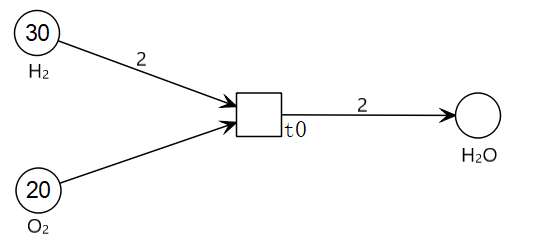
\includegraphics[width=0.5\columnwidth]{fig47}
		\caption{A Petri net example that models the chemical reaction, $2H_2+O_2\to 2H_2O$.}
		\label{fig:PNexample}
	\end{center}
\end{figure}



\subsection{Continuous Petri nets}

A continuous Petri net (CPN) \cite{BGH+08} is a variant of Petri nets. In a CPN model, the values identified on places are non-negative real values (no longer required to be non-negative integer values), which usually model the concentrations of species.
In fact, a CPN offer a graphical representation of a system of ODEs.

Let us continue to use the chemical reaction, $2H_2+O_2\to 2H_2O$ as an example to illustrate CPNs. The structure of the CPN model is exactly like the one given in Figure \ref{fig:PNexample}. Besides, we associate a kinetic rate, e.g., 0.1, with the transition $t$ by adopting a mass action law, represented as MassAction(0.1).
Here MassAction() is a macro that generates the rate function of a transition using its preplaces and taking a parameter as its argument. For example, MassAction(0.1) for transition $t$ generates a rate function, $0.1*H_2^{2}*O_2$. 
The set of ODEs underlying the CPN model given in Figure \ref{fig:PNexample} is shown in Table \ref{tab:ODEs-PN}.


\begin{table}[!hbt]
	\begin{center}
		\caption{ODEs of the CPN model given in Figure \ref{fig:PNexample}.}
		\label{tab:ODEs-PN}
		\begin{tabular}{|c|c|}
			\hline
			Species&ODE\\
			\hline
			$H_2$&$dH_2/dt=-2*(0.1*H_2^2*O_2)$\\
			\hline
			$O_2$&$dO_2/dt=-1*(0.1*H_2^2*O_2)$\\
			\hline
			$H_2O$&$dH_2O/dt=2*(0.1*H_2^2*O_2)$\\
			\hline
		\end{tabular}
	\end{center}
\end{table}


\subsection{Fuzzy logic}
Fuzzy logic \cite{Zad65,WRK07} is a form of many-valued logic in which the truth values of variables may be any real number between 0 and 1. It is employed to handle the concept of partial truth, where the truth value may range between completely true and completely false. By contrast, in Boolean logic, the truth values of variables may only be the integer values 0 or 1. Fuzzy logic is based on the observation that people make decisions based on imprecise and non-numerical information, and fuzzy sets are mathematical means of representing vagueness and imprecise information. 

Two widely used fuzzy inference systems are Mamdani and T-S inference systems.
In the following, we will briefly introduce these two systems.




\subsubsection{Mamdani fuzzy inference}
Mamdani fuzzy inference \cite{Mamdani74} is one of the most commonly used fuzzy inference systems and was among the first control systems built using fuzzy set theory. It expects the output membership functions to be fuzzy sets, which are then defuzzified to obtain crisp output values. The diagram of the Mamdani fuzzy inference system is shown in Figure \ref{fig:diagram-Mamdani}, which involves the following four components: fuzzification, fuzzy rule base, fuzzy inference engine and defuzzification. An example is also given in Figure \ref{fig:example -Mamdani} to illustrate the reasoning process of the Mamdani fuzzy inference system.

\begin{figure}[!hbt]
	\begin{center}
		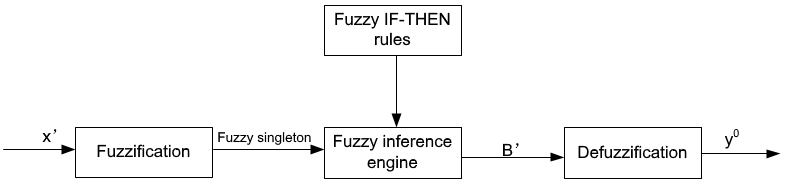
\includegraphics[width=\columnwidth]{fig48}
		\caption{Diagram of the Mamdani fuzzy inference system.}
		\label{fig:diagram-Mamdani}
	\end{center}
\end{figure}

\begin{figure}[!hbt]
	\begin{center}
		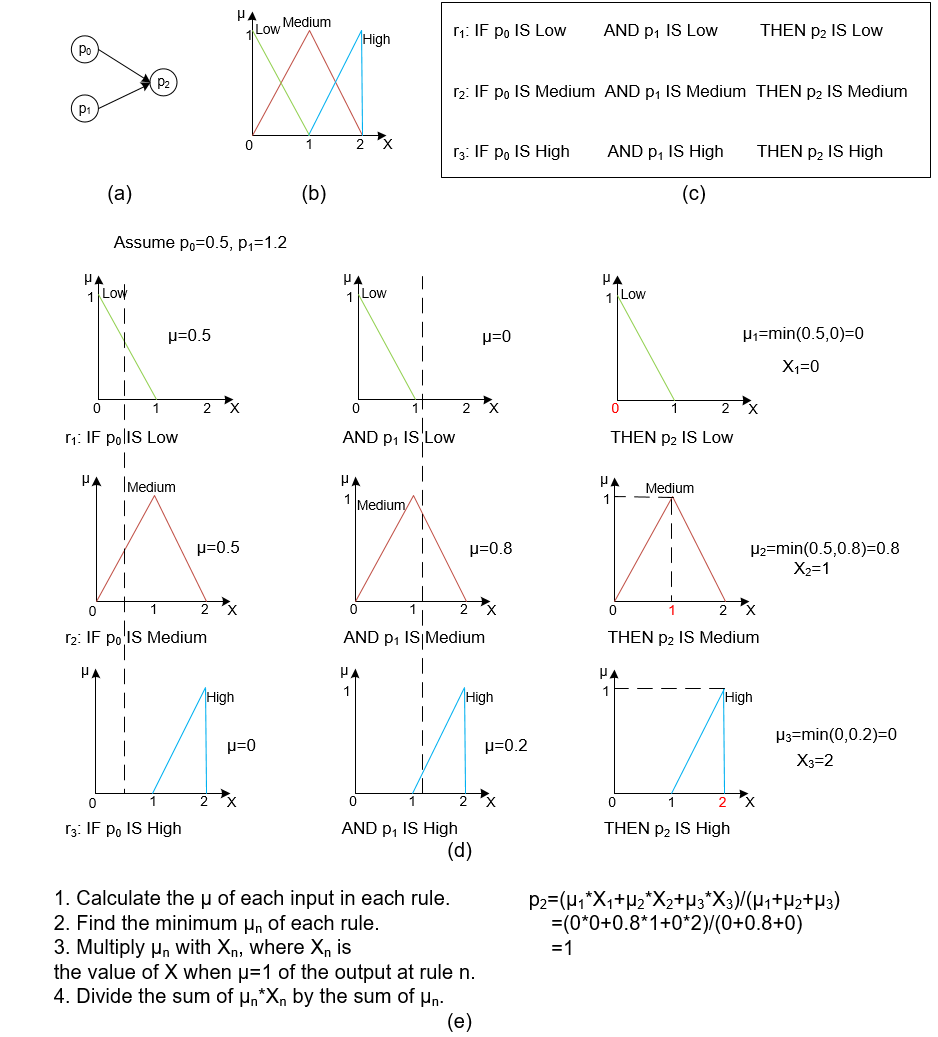
\includegraphics[width=\columnwidth]{fuzzy_logic_example}
		\caption{An example of the Mamdani fuzzy inference system.}
		\label{fig:example -Mamdani}
	\end{center}
\end{figure}

(1)Fuzzification
Fuzzification is used to fuzzify crisp input values into fuzzy values according to predefined membership functions for input variables. 
For example, for the model given in Figure \ref{fig:example -Mamdani}(a), p0 and p1 are inputs while p2 is the output. Three linguistic terms, Low, Medium and High, each taking a triangular fuzzy number, are defined for p0 to p2 (see Figure \ref{fig:example -Mamdani}(b)). We assume that the minimum and maximum values of p0, p1 and p2 are 0 and 2, respectively. In the fuzzy membership functions shown in Figure \ref{fig:example -Mamdani}(b), $X$ indicates the value of each input and $\mu$ indicates the membership grade of the fuzzy set.

(2)Fuzzy rule base
The rule base is a collection of fuzzy rules that are defined for a specific application. 
For example, for the model given in Figure \ref{fig:example -Mamdani}(a), we can define the fuzzy rules given in Figure \ref{fig:example -Mamdani}(c).
A uniform format of the rules is:
\begin{center}
$r^r$: IF $x_1$ IS $A^r_1$ AND ... AND IF $x_n$ IS $A^r_n$ THEN $y^r$ IS ${B'}^r$.
\end{center}

(3)Fuzzy inference engine
Fuzzy inference engine is used to execute all applicable rules in the rule base to compute the fuzzy output values.
A detailed reasoning example is given in Figure \ref{fig:example -Mamdani}(d).

(4)Defuzzification
Defuzzification is used to defuzzify the fuzzy output values to get ``crisp'' output values.
See an example in Figure \ref{fig:example -Mamdani}(e).
 



\clearpage
\subsubsection{T-S Fuzzy Inference}

T-S fuzzy inference \cite{TS85} is also called Sugeno or Takagi-Sugeno-Kang fuzzy inference. This method is similar to the Mamdani one except the difference that the T-S' outputs are either crisp linear expressions or constants rather than fuzzy values. 
The uniform format of the T-S rules is
\begin{center}
	$r^r$: IF $x_1$ IS $A^r_1$ AND ... AND IF $x_n$ IS $A^r_n$ THEN $y^r=a^r_1x_1+...+a^r_nx_n+c^r$.
\end{center}
where $a^r_i$ is $i$th coefficient in $r$th rule and $c^r$ is a constant. 

The process of the T-S fuzzy inference system is shown in Figure \ref{fig:diagram-T-S}, which involves three components: fuzzification, fuzzy rule base, and fuzzy inference engine. An example is also given in Figure \ref{fig:example-T-S} to illustrate the reasoning process of the T-S fuzzy inference system.

\begin{figure}[!hbt]
	\begin{center}
		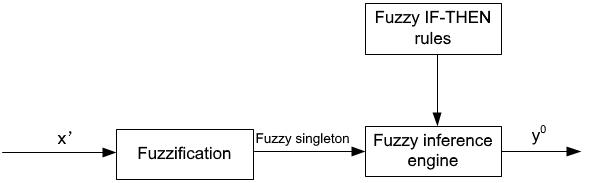
\includegraphics[width=0.7\columnwidth]{fig49}
		\caption{Diagram of the T-S fuzzy inference system.}
		\label{fig:diagram-T-S}
	\end{center}
\end{figure}

\begin{figure}[!hbt]
	\begin{center}
		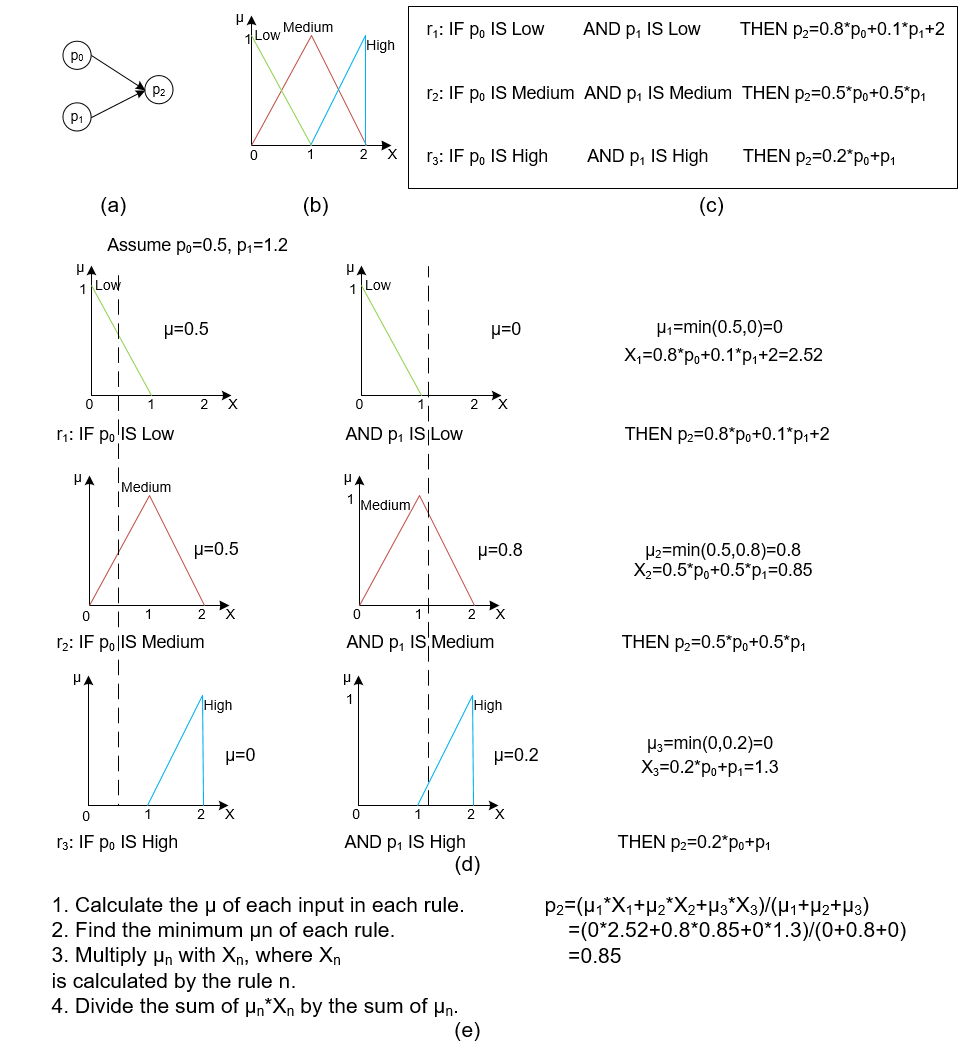
\includegraphics[width=\columnwidth]{fuzzy_logic_example1}
		\caption{An example of the T-S fuzzy inference system.}
		\label{fig:example-T-S}
	\end{center}
\end{figure}



\subsection{Fuzzy continuous Petri nets}
Adding fuzzy logic to continuous Petri nets gets fuzzy continuous Petri nets \cite{LHG18}, which make the Petri nets more powerful. For example, if we want to get the value of $H_2O$ using fuzzy logic, but ODE no longer works for $H_2O$, then the value of $H_2O$ can be obtained by fuzzy logic. 

Please note that when using fuzzy logic in fuzzy continuous Petri nets, the value we obtained is not the value of the variable, but the amount of change within the step. The change value of $H_2O$ of current time step is obtained by the values of $H_2$ and $O_2$ of previous time step. 

The result might be a little different from ODE. If the values of $H_2$ and $O_2$ are down to 18 and 14, the ODE result of $H_2O$ is 12, while in fuzzy logic, the result of $H_2O$ might be 11.8. 
\begin{figure}[!hbt]
	\begin{center}
		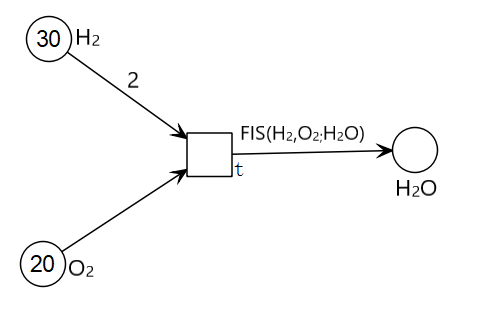
\includegraphics[width=0.5\columnwidth]{fig50}
		\caption{Example of fuzzy continuous Petri nets.}
		\label{fig:Example of fuzzy continuous Petri nets}
	\end{center}
\end{figure}


\subsection{FCPN tool}

The tool provides modeling and simulation functions of fuzzy continuous Petri nets for researchers in the field of systems biology.
It includes three main functions: continuous Petri net modeling, fuzzy (Mamdani \& T-S) modeling, and hybrid simulation. 
The aim of this software is to give an easy-to-use graphical tool for the construction and simulation of FCPN models.

We offer the Windows, Linux, and macOS (beta) versions of the software. To use the software, please follow the instruction in \href{https://github.com/liufei2016/fcpn/blob/master/README.md}{README.md} and download the corresponding version of the tool.


\subsection{Features - overview}
Before exploring all features in detail in the following sections, we will give a brief overview for the expected features here.

\subsubsection{Features for modeling}
\begin{itemize}
	\item Concise and efficient interface design.
	\item Drawing of the Petri net graph as usual.
	\item Flexible user-defined functions.
	\item Multiple fuzzy logic choices.
	\item Simple and fast fuzzy logic settings.
	\item Save as Petri Net Markup Language (PNML) format
	\item Rich shortcut settings, such as undo, redo, save, print, etc.
\end{itemize}


\subsubsection{Features for simulation}
\begin{itemize}
	\item Highly automated simulation process.
	\item Diversified export of simulation results.
	\item Custom simulation result drawing.
\end{itemize}






%Section 2
\clearpage
\section{Modeling}

This section will present a general step-by-step procedure for how to construct an FCPN model. We will take the chemical reaction $2H_2+O_2\to 2H_2O$ as an example \cite{Mur89} for the illustration of the procedure.

\subsection{An overview of the main interface}
Figure \ref{fig:Maininterface} shows the main interface of the software. 
The menu bar is on the top and the tool bar is on the left, which facilitates us to create the net conveniently. The tools from top to bottom include ``new'', ``open", ``save", ``save as", ``print", ``undo", ``redo", ``delete a node", ``normal cursor", ``create a new place", ``create a new transition", ``create a new arc", and ``start simulation". 

The top window is used to draw the net and the bottom window to output a log. The bottom right slider can be used to zoom in or zoom out a net.

\begin{figure}[!hbt]
	\begin{center}
		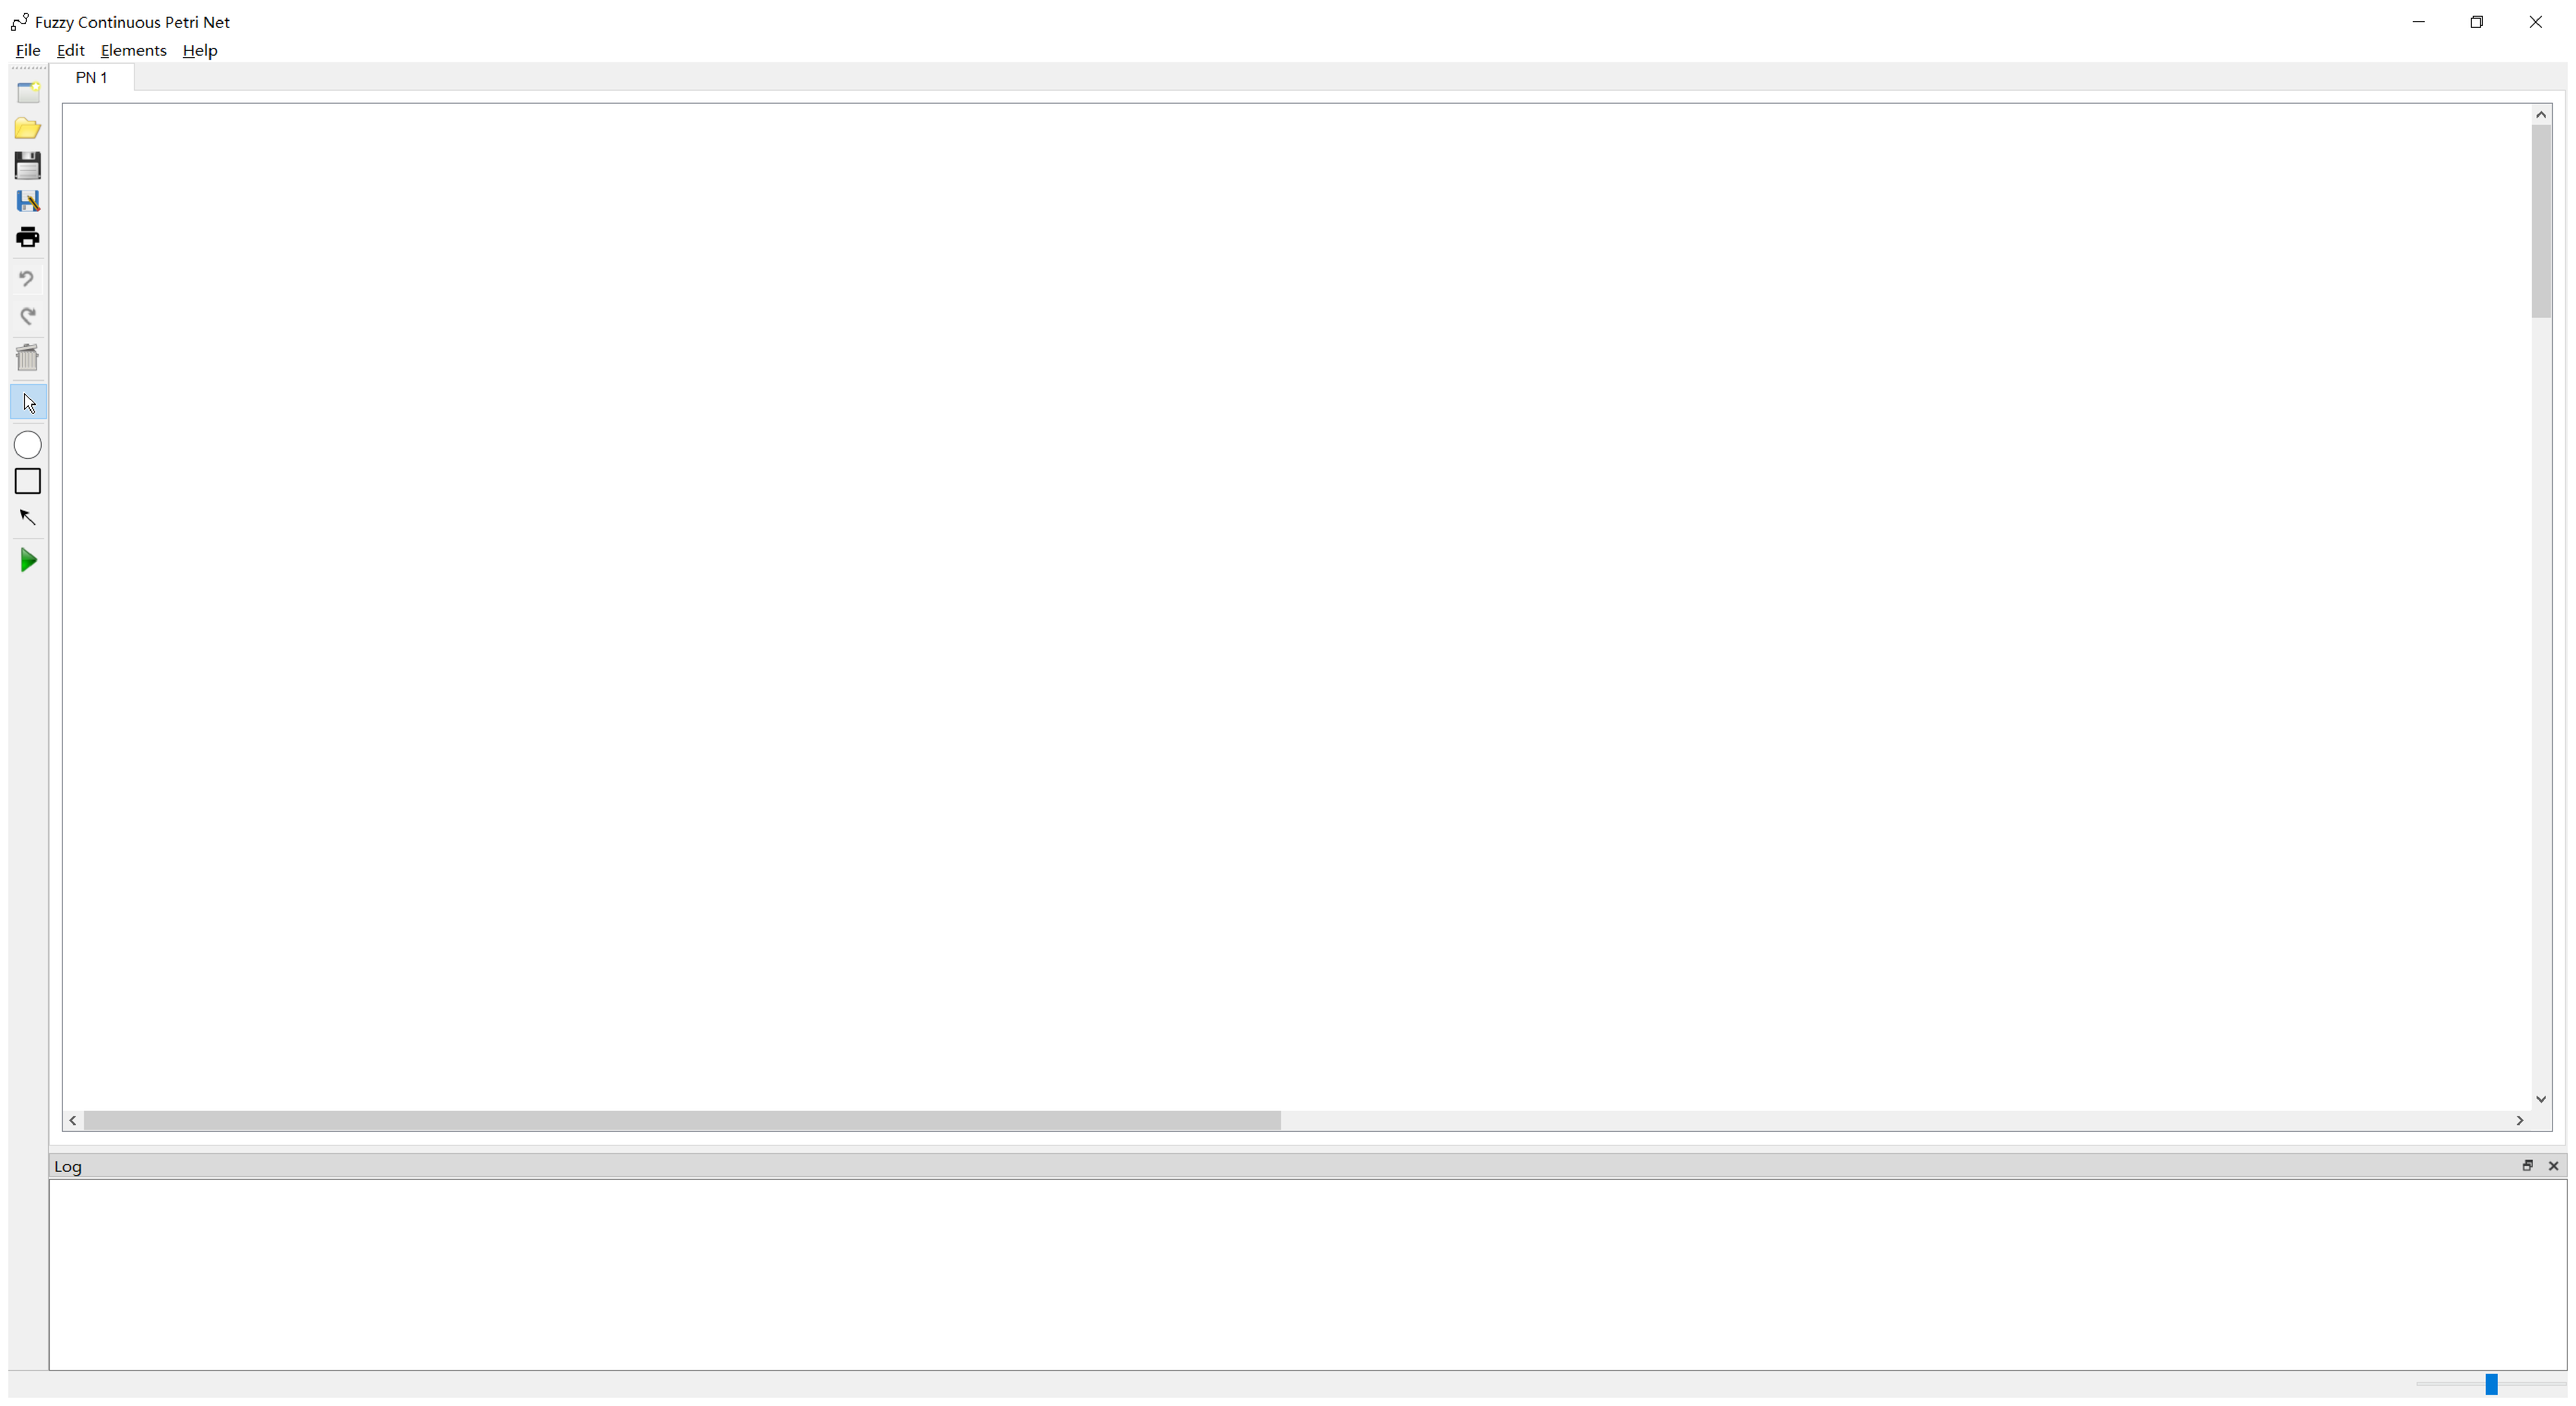
\includegraphics[width=\columnwidth]{fig1}
		\caption{Main interface of the software.}
		\label{fig:Maininterface}
	\end{center}
\end{figure}



\subsection{Draw a net}
We can draw a net using the following steps taking Figure \ref{fig:drawnet} as an example: 

\begin{itemize}
	\item Left click the place button (the circle on the tool bar).
	\item Put three places on the palette where you want by left clicking the mouse.
	\item Left click the transition button (the square on the tool bar).
	\item Put one transition on the palette where you want by left clicking the mouse.
	\item Left click the arc button (the arrow on the tool bar).
	\item Left click a place, press the mouse and hold, move the mouse to a transition, and then release the mouse. In this way you can draw an arrow from a place to a transition or vice versa.
	\item Repeating these steps, an FCPN can be constructed; see Figure \ref{fig:drawnet}.
\end{itemize}


\begin{figure}[!hbt]
	\begin{center}
		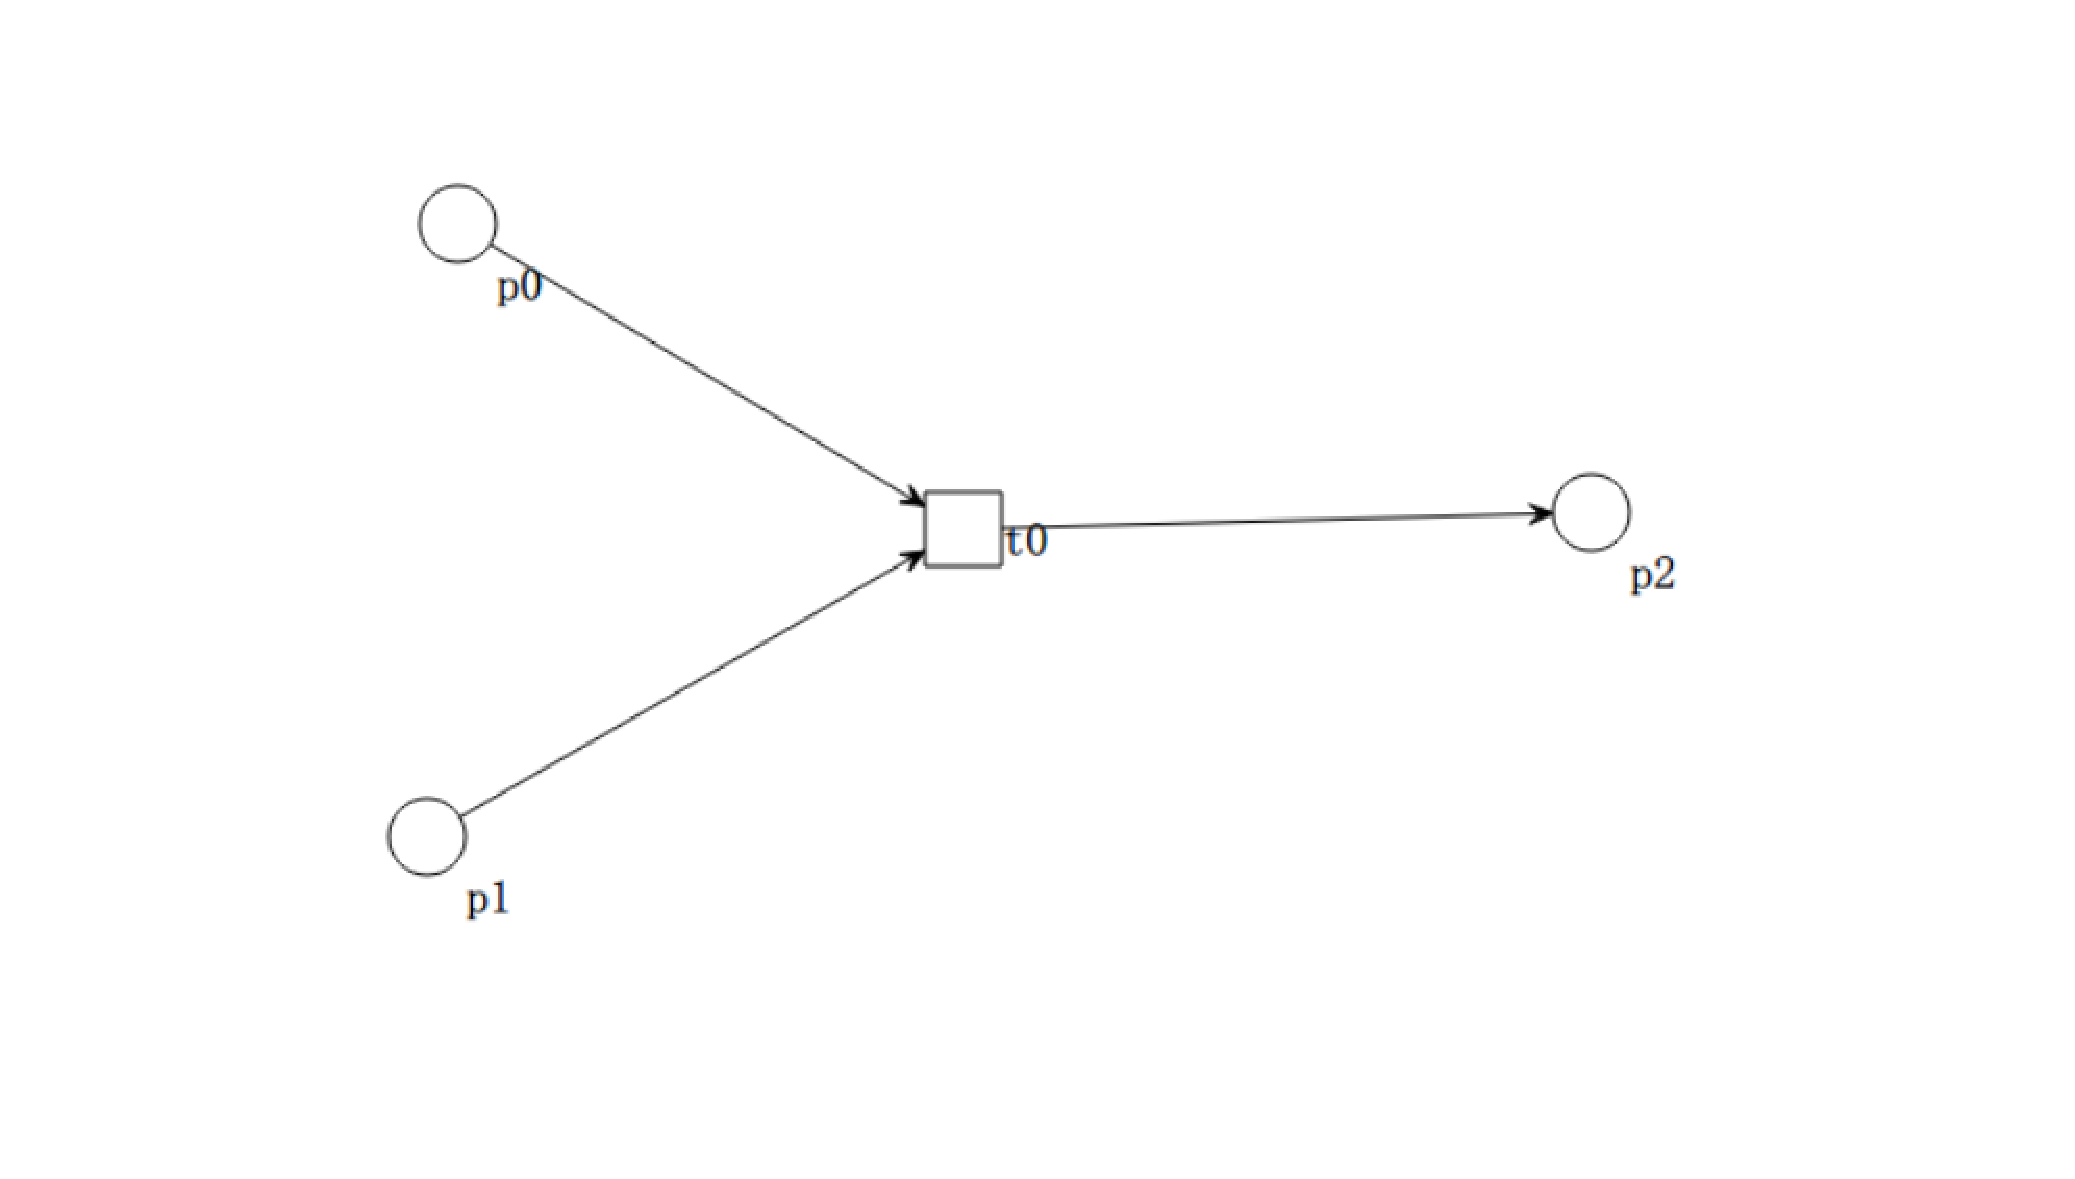
\includegraphics[width=0.6\columnwidth]{fig2}
		\caption{Draw the net.}
		\label{fig:drawnet}
	\end{center}
\end{figure}


\subsubsection{Edit a place}
We can edit the properties of a place in the following way:

\begin{itemize}
	\item Double click the place on the palette.
	\item A window named Place Attributes (Figure \ref{fig:editplace}) will show.
	\item Change the Name and Marking.
	\item After editing, left click the OK button.
\end{itemize}

For example, in Figure \ref{fig:drawnet}, we change the names of p0, p1, and p2 to H2, O2, and H2O, respectively, and change the markings of p0, p1, and p2 to 30, 20, and 0, respectively. Please note that the name of each place should be unique and a marking should be a non-negative real number.

\begin{figure}[!hbt]
	\begin{center}
		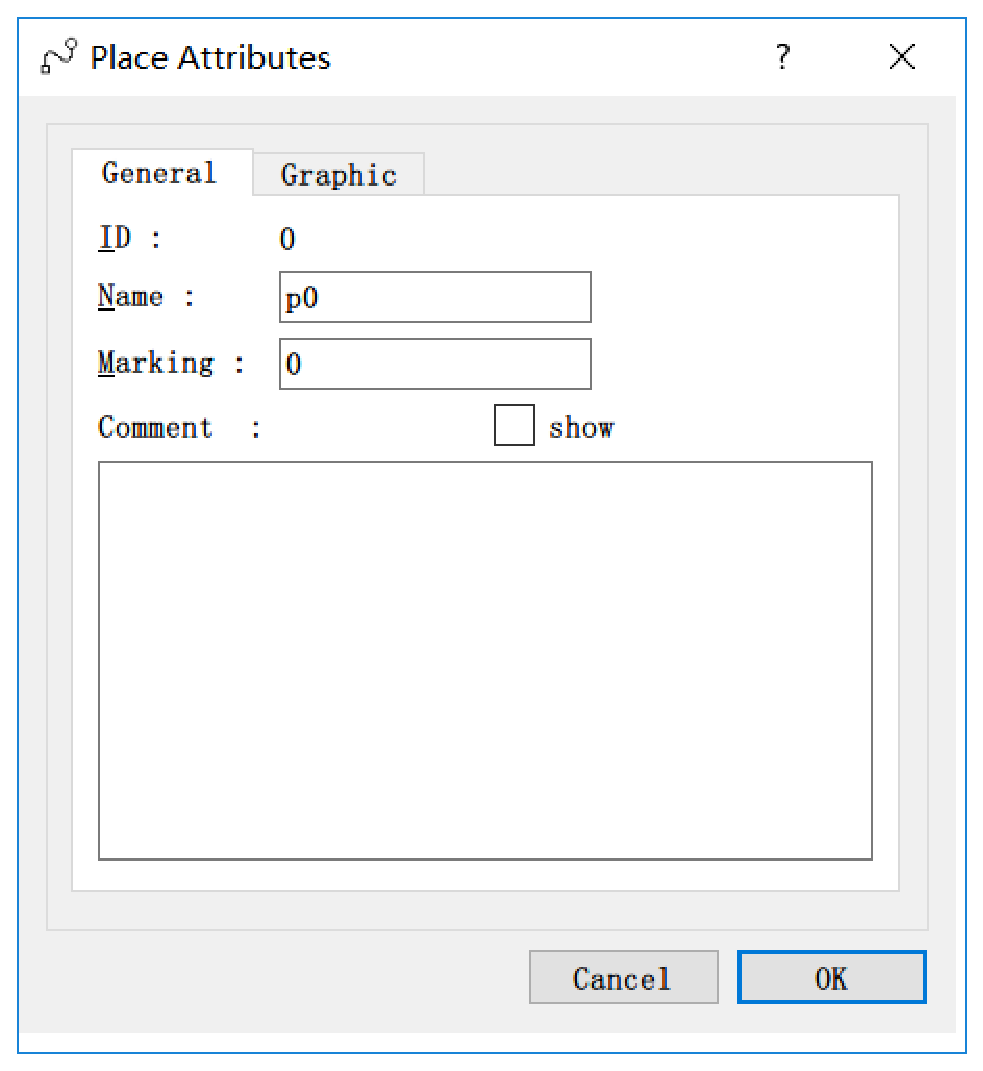
\includegraphics[width=0.8\columnwidth]{fig3}
		\caption{Edit a place.}
		\label{fig:editplace}
	\end{center}
\end{figure}


\subsubsection{Edit a transition}
We can edit the properties of a transition in the following way:

\begin{itemize}
	\item Double click the transition on the palette.
	\item A window named Transition Attributes (Figure \ref{fig:edittransition}) will show.
	\item Change the Name and Function.
	\item After editing, left click the OK button.
\end{itemize}

For example, in Figure \ref{fig:drawnet}, we change the function of t0 from the default MassAction(1) to MassAction(0.1). Please note that the name of each transition should be unique and the function should be an expression like a constant ``1", an expression containing its preplaces``0.1*H2", or a mass action ``MassAction(0)". Remember not to change the ``MassAction(1)" to ``massaction(1)" or something like that as we distinguish the upper and lower case letters. And do not leave the function empty; otherwise a compile error will occur.

\begin{figure}[!hbt]
	\begin{center}
		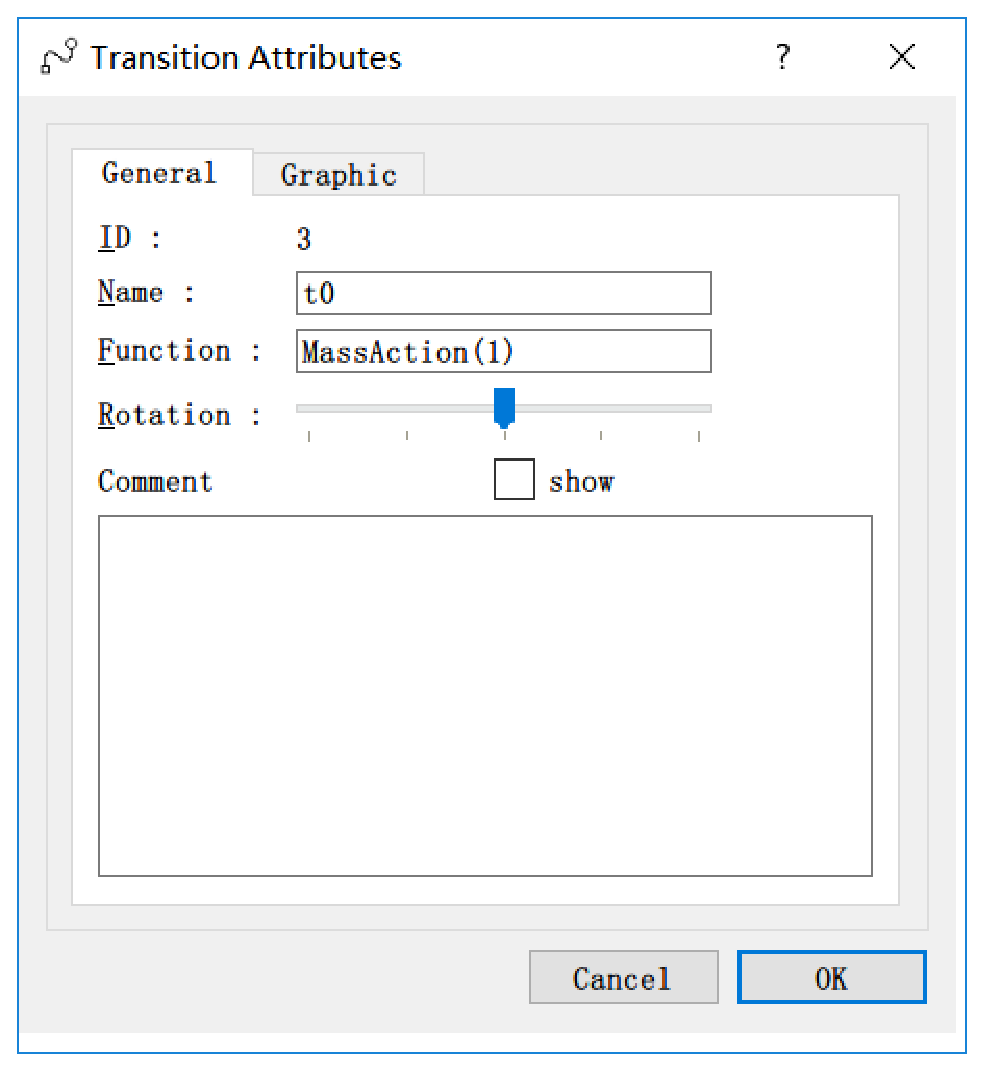
\includegraphics[width=0.8\columnwidth]{fig4}
		\caption{Edit a ransition.}
		\label{fig:edittransition}
	\end{center}
\end{figure}



\subsubsection{Edit an arc}
We can edit th properties of an arc in the following way:
\begin{itemize}
	\item Double click the arc on the palette.
	\item A window named Arc Attributes (Figure \ref{fig:editarc}) will show.
	\item Change the Expression.
	\item After editing, left click the OK button.
\end{itemize}

For example, in Figure \ref{fig:drawnet}, we change the expression of arc from p0 (H2) to t0 to 2. Please note that the expression should be like ``1", ``H2", if you don't want use fuzzy logic, and do not leave the expression empty. Otherwise a compile error might occur. 

\begin{figure}[!hbt]
	\begin{center}
		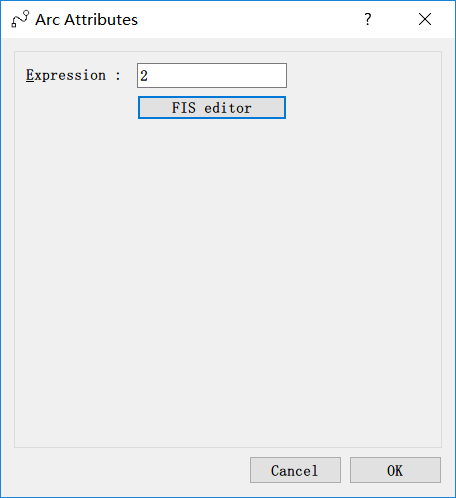
\includegraphics[width=0.8\columnwidth]{fig5}
		\caption{Edit an arc.}
		\label{fig:editarc}
	\end{center}
\end{figure}



\subsubsection{Use FIS}
FIS is the abbreviation of the fuzzy inference system. We provide two kinds of FISs: Mamdani and T-S. The steps are slightly different between Mamdani and T-S settings. Here are the steps for using Mamdani inference system: 

 \begin{figure}[!hbt]
 	\begin{center}
 		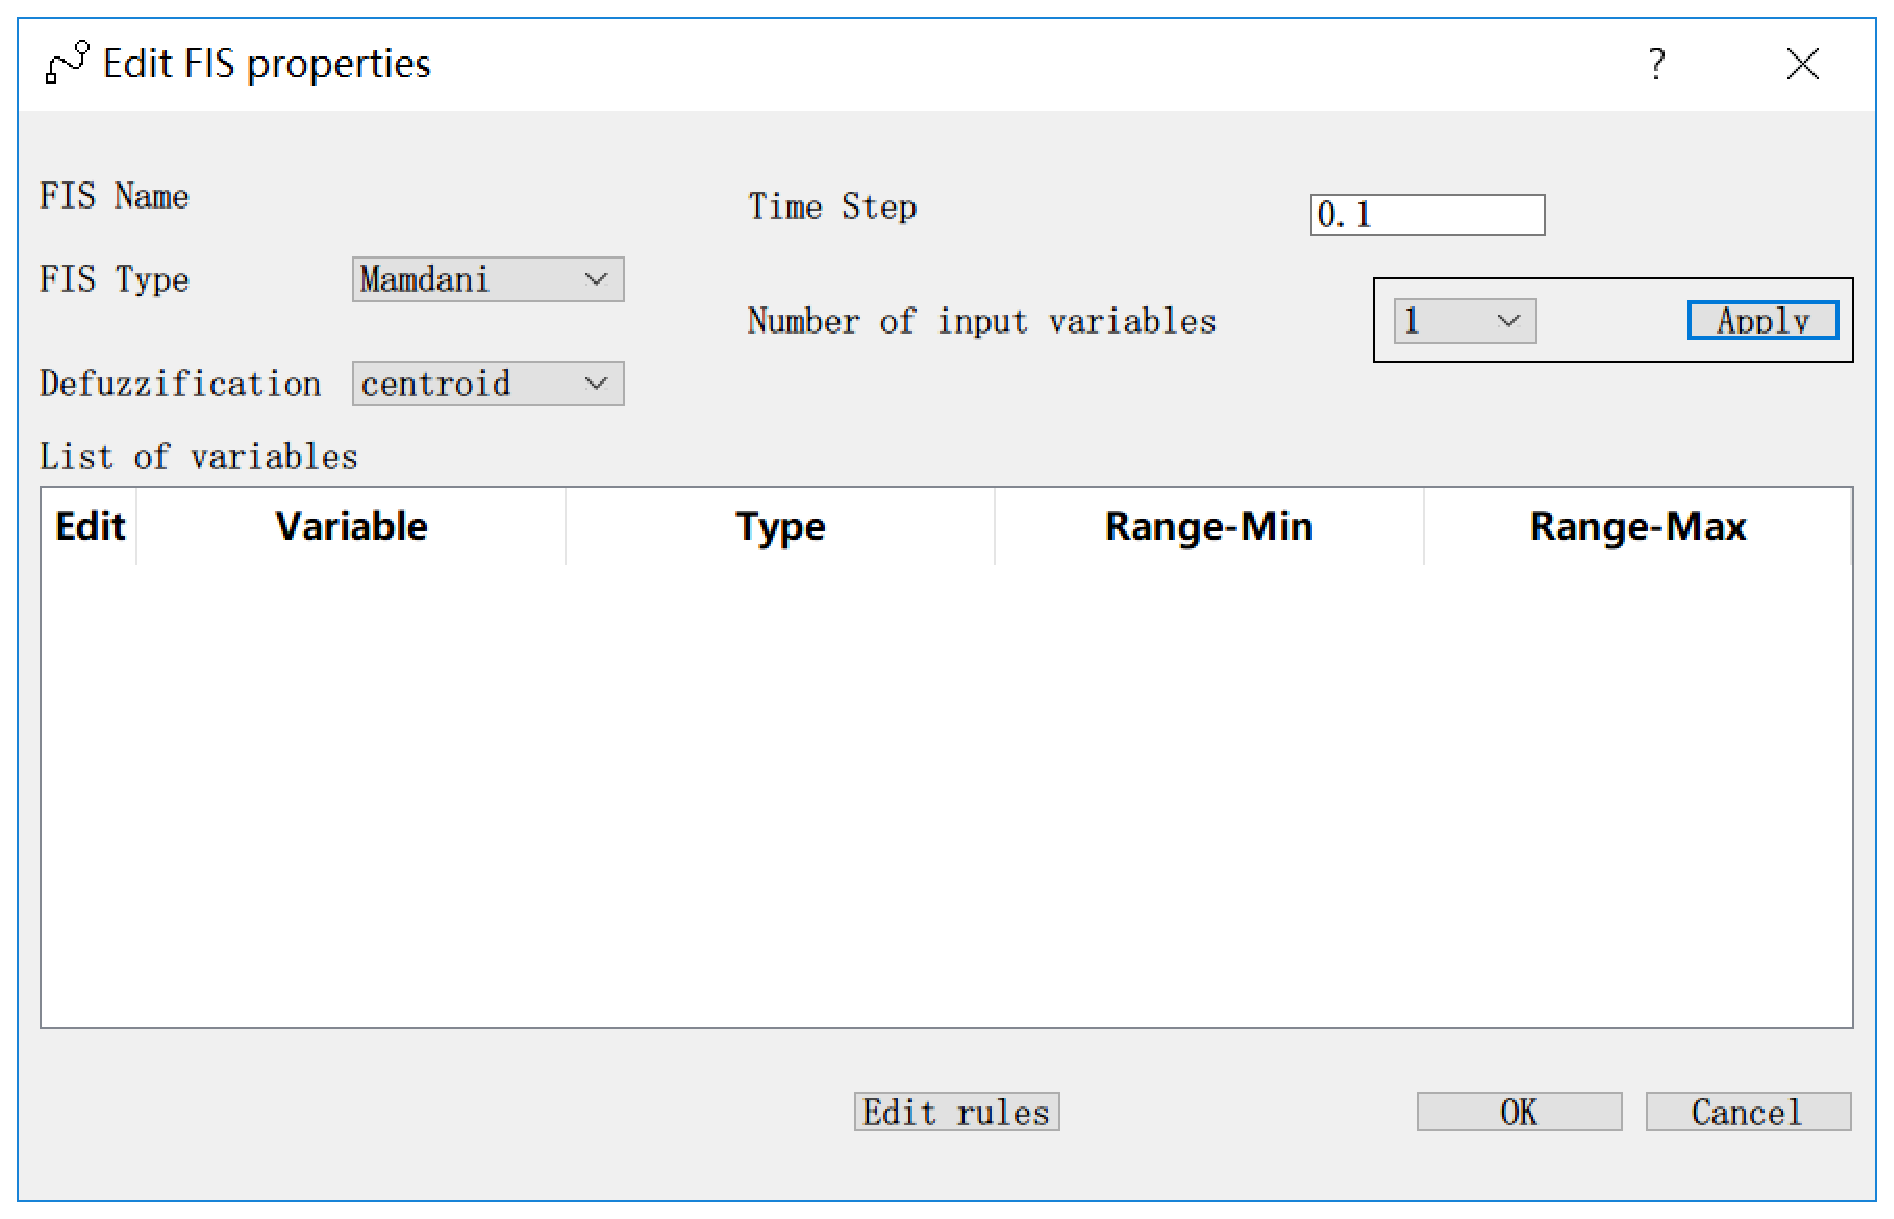
\includegraphics[width=\columnwidth]{fig7}
 		\caption{FIS editor.}
 		\label{fig:FIS editor}
 	\end{center}
 \end{figure}

\begin{itemize}
	\item Double click the arc from t0 to p2 (H2O).
	\item Click the FIS editor button.
	\item Choose Mamdani FIS Type.
	\item Enter the time step and select the number of input variables.
	\item Click the Apply button.
	\item Choose each variable and its membership function type (either triangular or Gauss fuzzy numbers) in the table.
	\item Specify the minimum and maximum values for input variables.
	\item Specify the minimum and maximum increment/decrement values at a time step for the output.
\end{itemize}

Make sure we only allow to specify one output variable whose type is PN\_OUTPUT, and it should be the variable connected by the arc you chose. In this example, that's p2 (H2O). The values are shown in Figure \ref{fig:Edit variables}.

\begin{figure}[!hbt]
	\begin{center}
		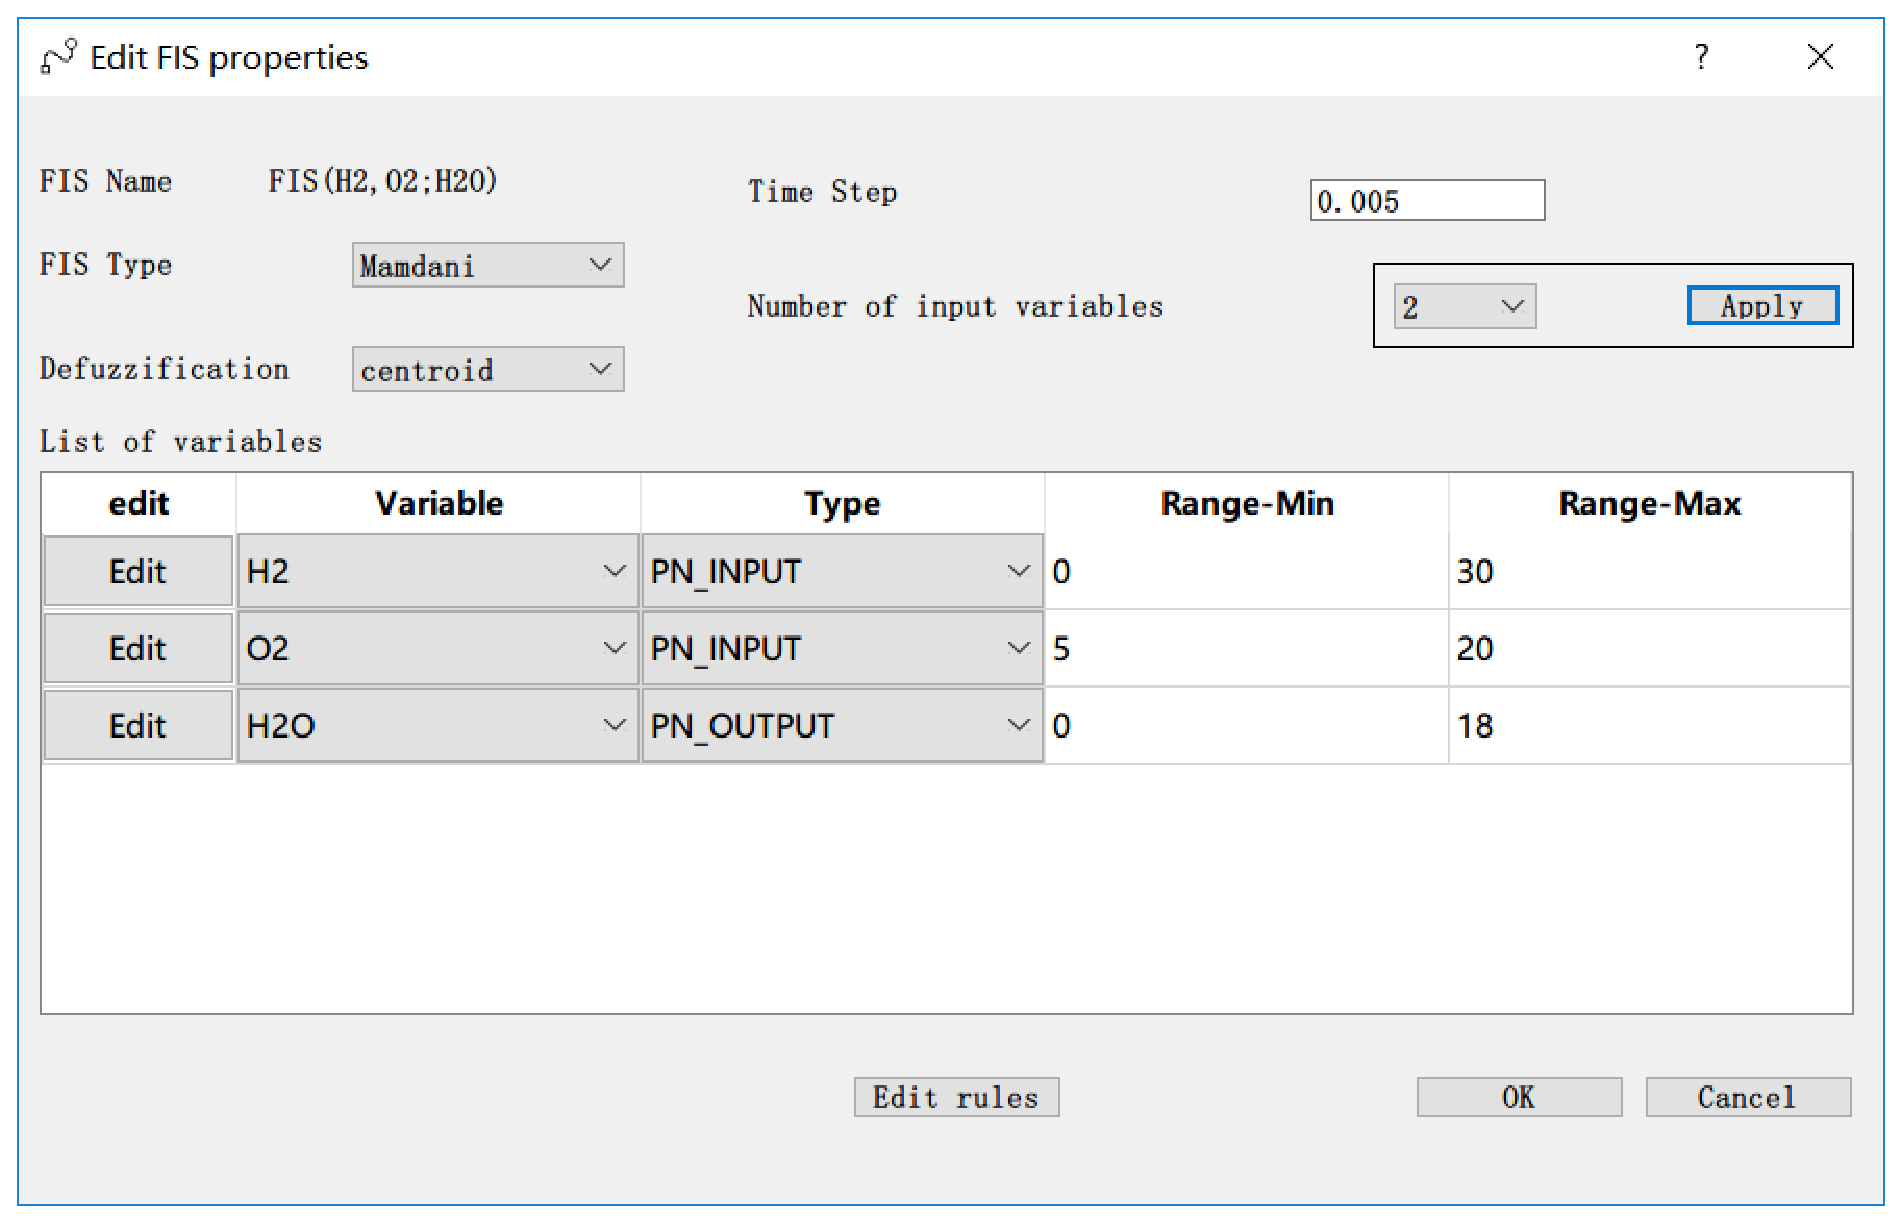
\includegraphics[width=\columnwidth]{fig8}
		\caption{Edit variables.}
		\label{fig:Edit variables}
	\end{center}
\end{figure}

Now we need to edit each variable's membership functions. Here are the steps:
\begin{itemize}
	\item Click the Edit button on the first column.
	\item Choose the number of linguistic variables.
	\item Click the Apply button and the according label will show.
	\item For each function, enter the values of left/average, center/variance and right/-, which specify the parameters that are needed by triangular/Gauss fuzzy numbers.
	\item Click the Show Plot button to see whether it is the graph you want.
	\item Click the OK button to save the change and close the window.
	\item Repeat these steps to edit each variable.
\end{itemize}

We provide the user to choose the number (2, 3, 5, 7) of linguistic terms. The membership functions are shown in Figure \ref{fig:Membership functions of H2}, \ref{fig:Membership functions of O2}, and \ref{fig:Membership functions of H2O}.

\begin{figure}[!hbt]
	\begin{center}
		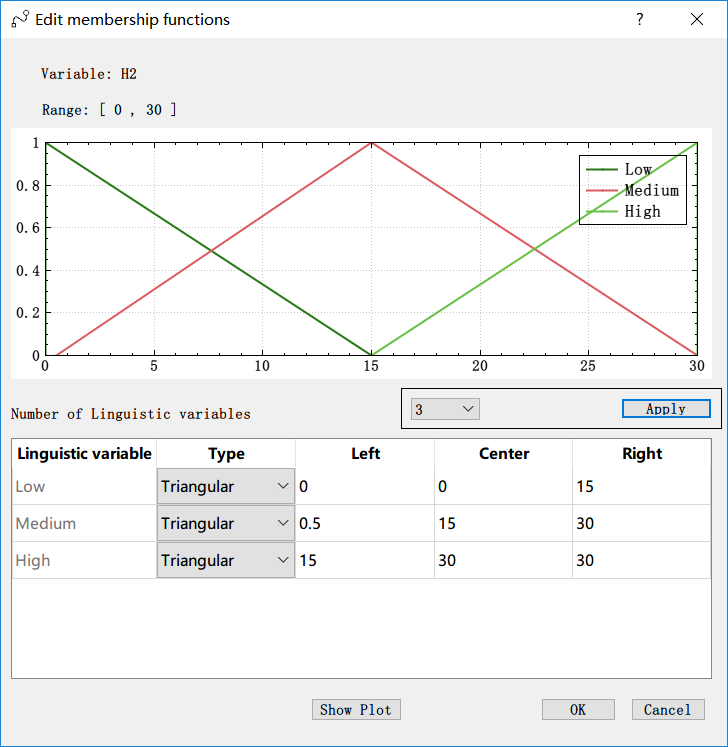
\includegraphics[width=0.8\columnwidth]{fig9}
		\caption{Membership functions of H2.}
		\label{fig:Membership functions of H2}
	\end{center}
\end{figure}

\begin{figure}[!hbt]
	\begin{center}
		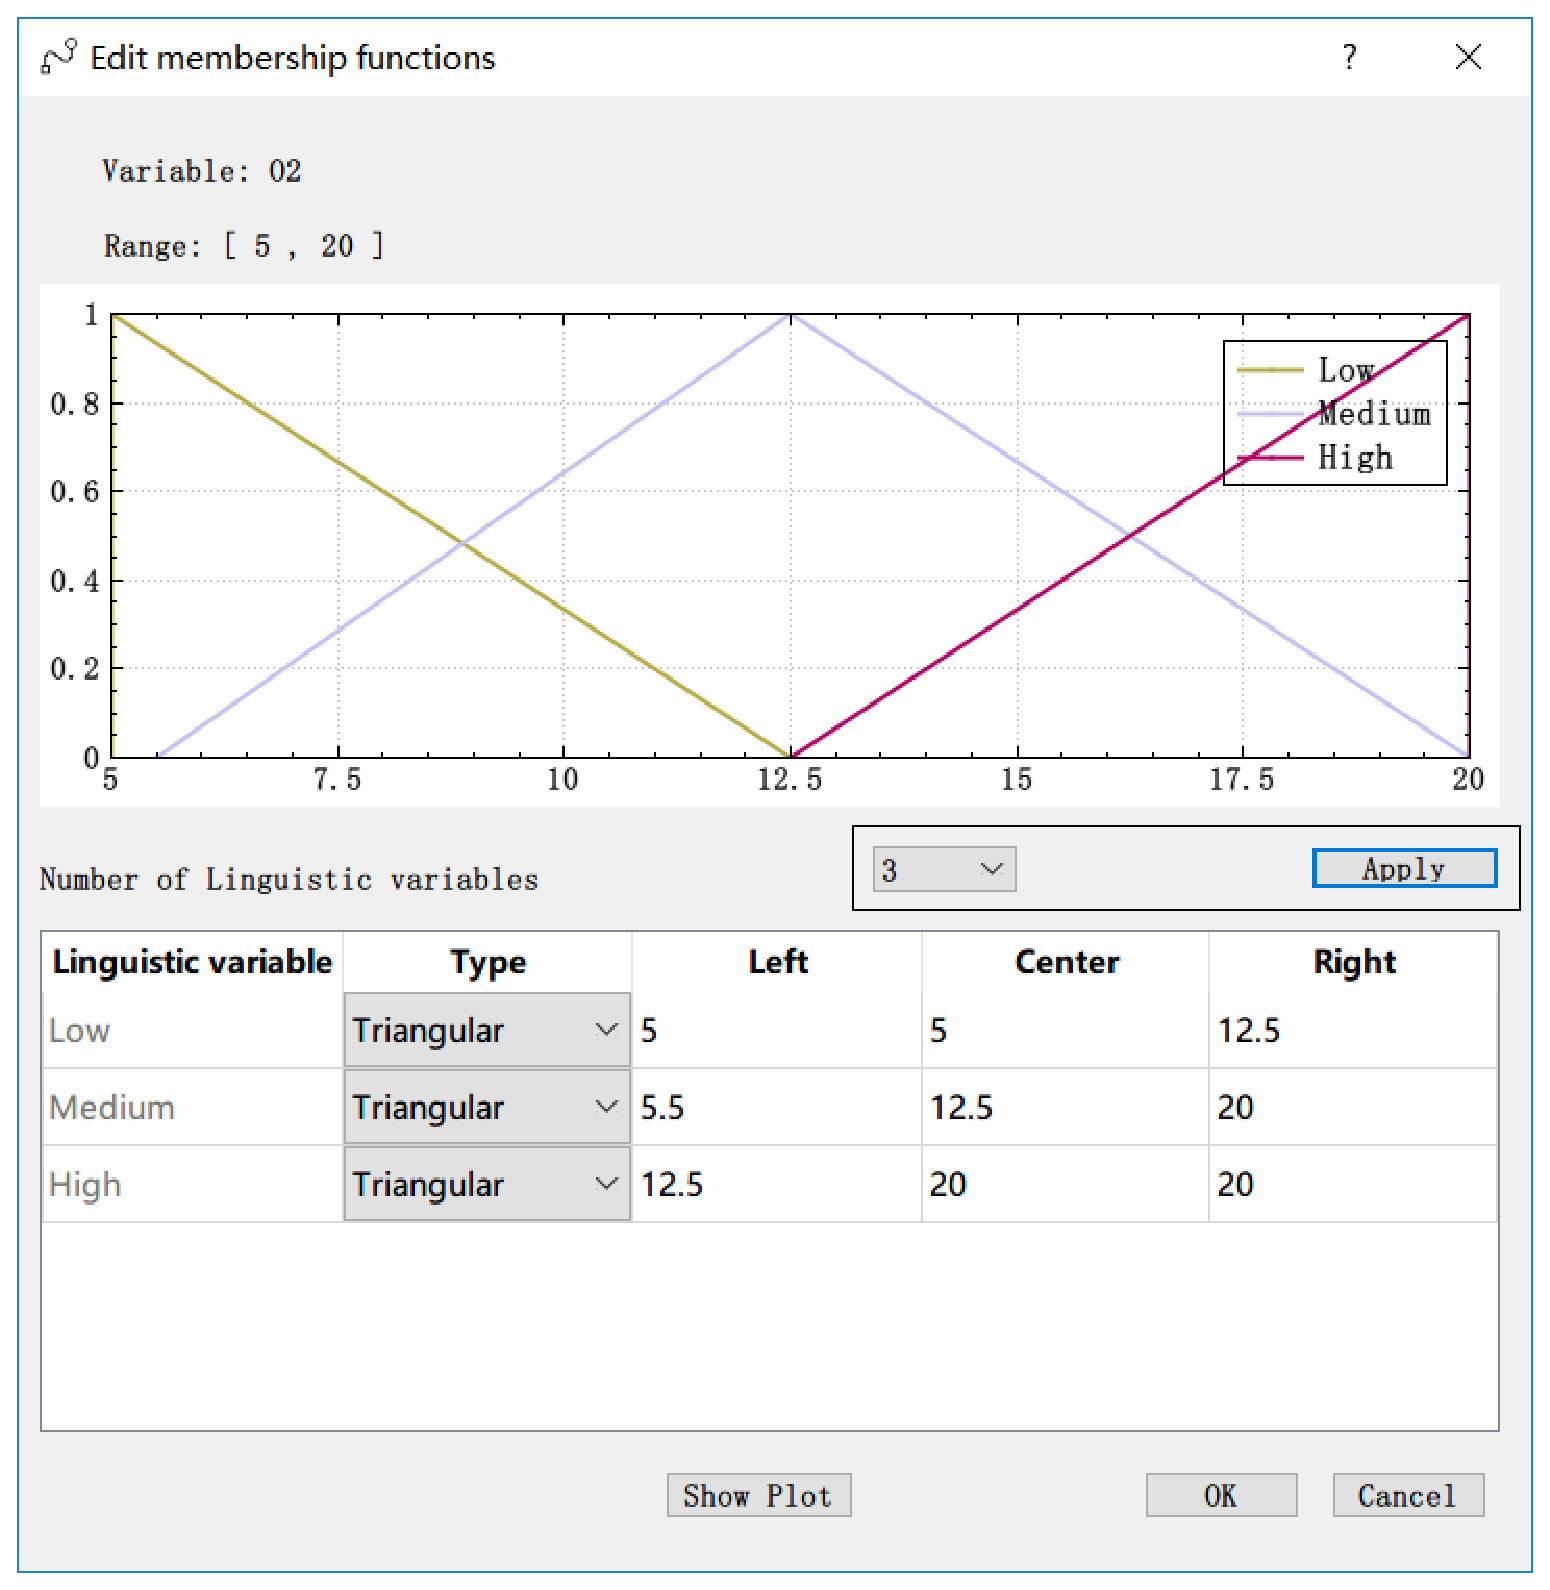
\includegraphics[width=0.8\columnwidth]{fig9_1}
		\caption{Membership functions of O2.}
		\label{fig:Membership functions of O2}
	\end{center}
\end{figure}

\begin{figure}[!hbt]
	\begin{center}
		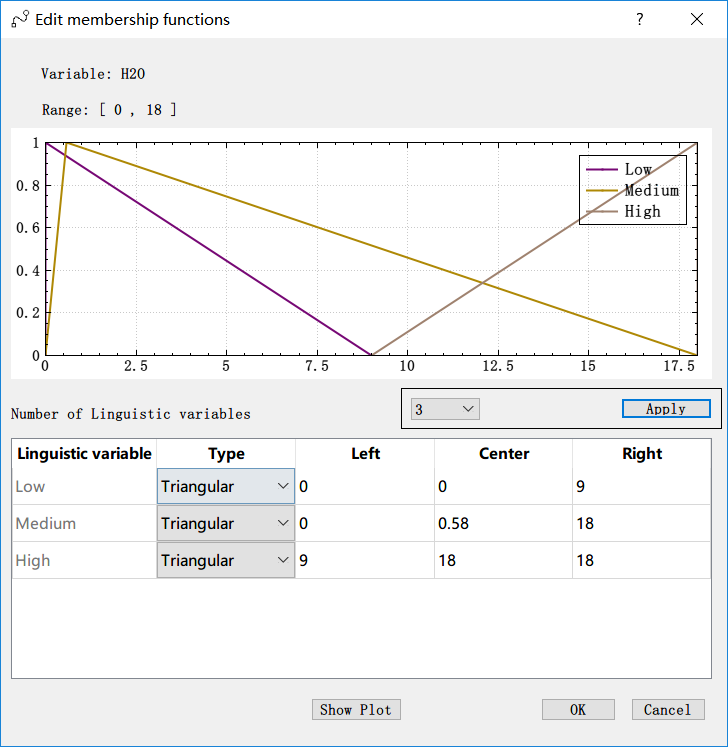
\includegraphics[width=0.8\columnwidth]{fig9_2}
		\caption{Membership functions of H2O.}
		\label{fig:Membership functions of H2O}
	\end{center}
\end{figure}


\clearpage
Next we should edit rules by following these steps:
\begin{itemize}
	\item Click the Edit rules button on the bottom.
	\item Select the items of a rule, and left click Add rule button to add it.
	\item Repeat the previous step to add rules.
	\item Click the OK button to save the changes and close the window.
\end{itemize}

We can select a row and left click Change rule button to change the rule you selected. Choosing a row and left clicking the Delete rule button can be used to delete the rule.

Make sure that the meanings of inputs' linguistic variables and output's linguistic variables are different. For example, as is shown in Figure \ref{fig:Edit rules}, one of the rules is - IF H2 IS Low AND O2 IS Low Then H20 IS Low. This means that if the value of H2 is Low and the value of O2 is Low, then the increment of H2O is Low, not meaning that the value of H2O will be low.

The rules are shown in Figure \ref{fig:Edit rules}.

\begin{figure}[!hbt]
	\begin{center}
		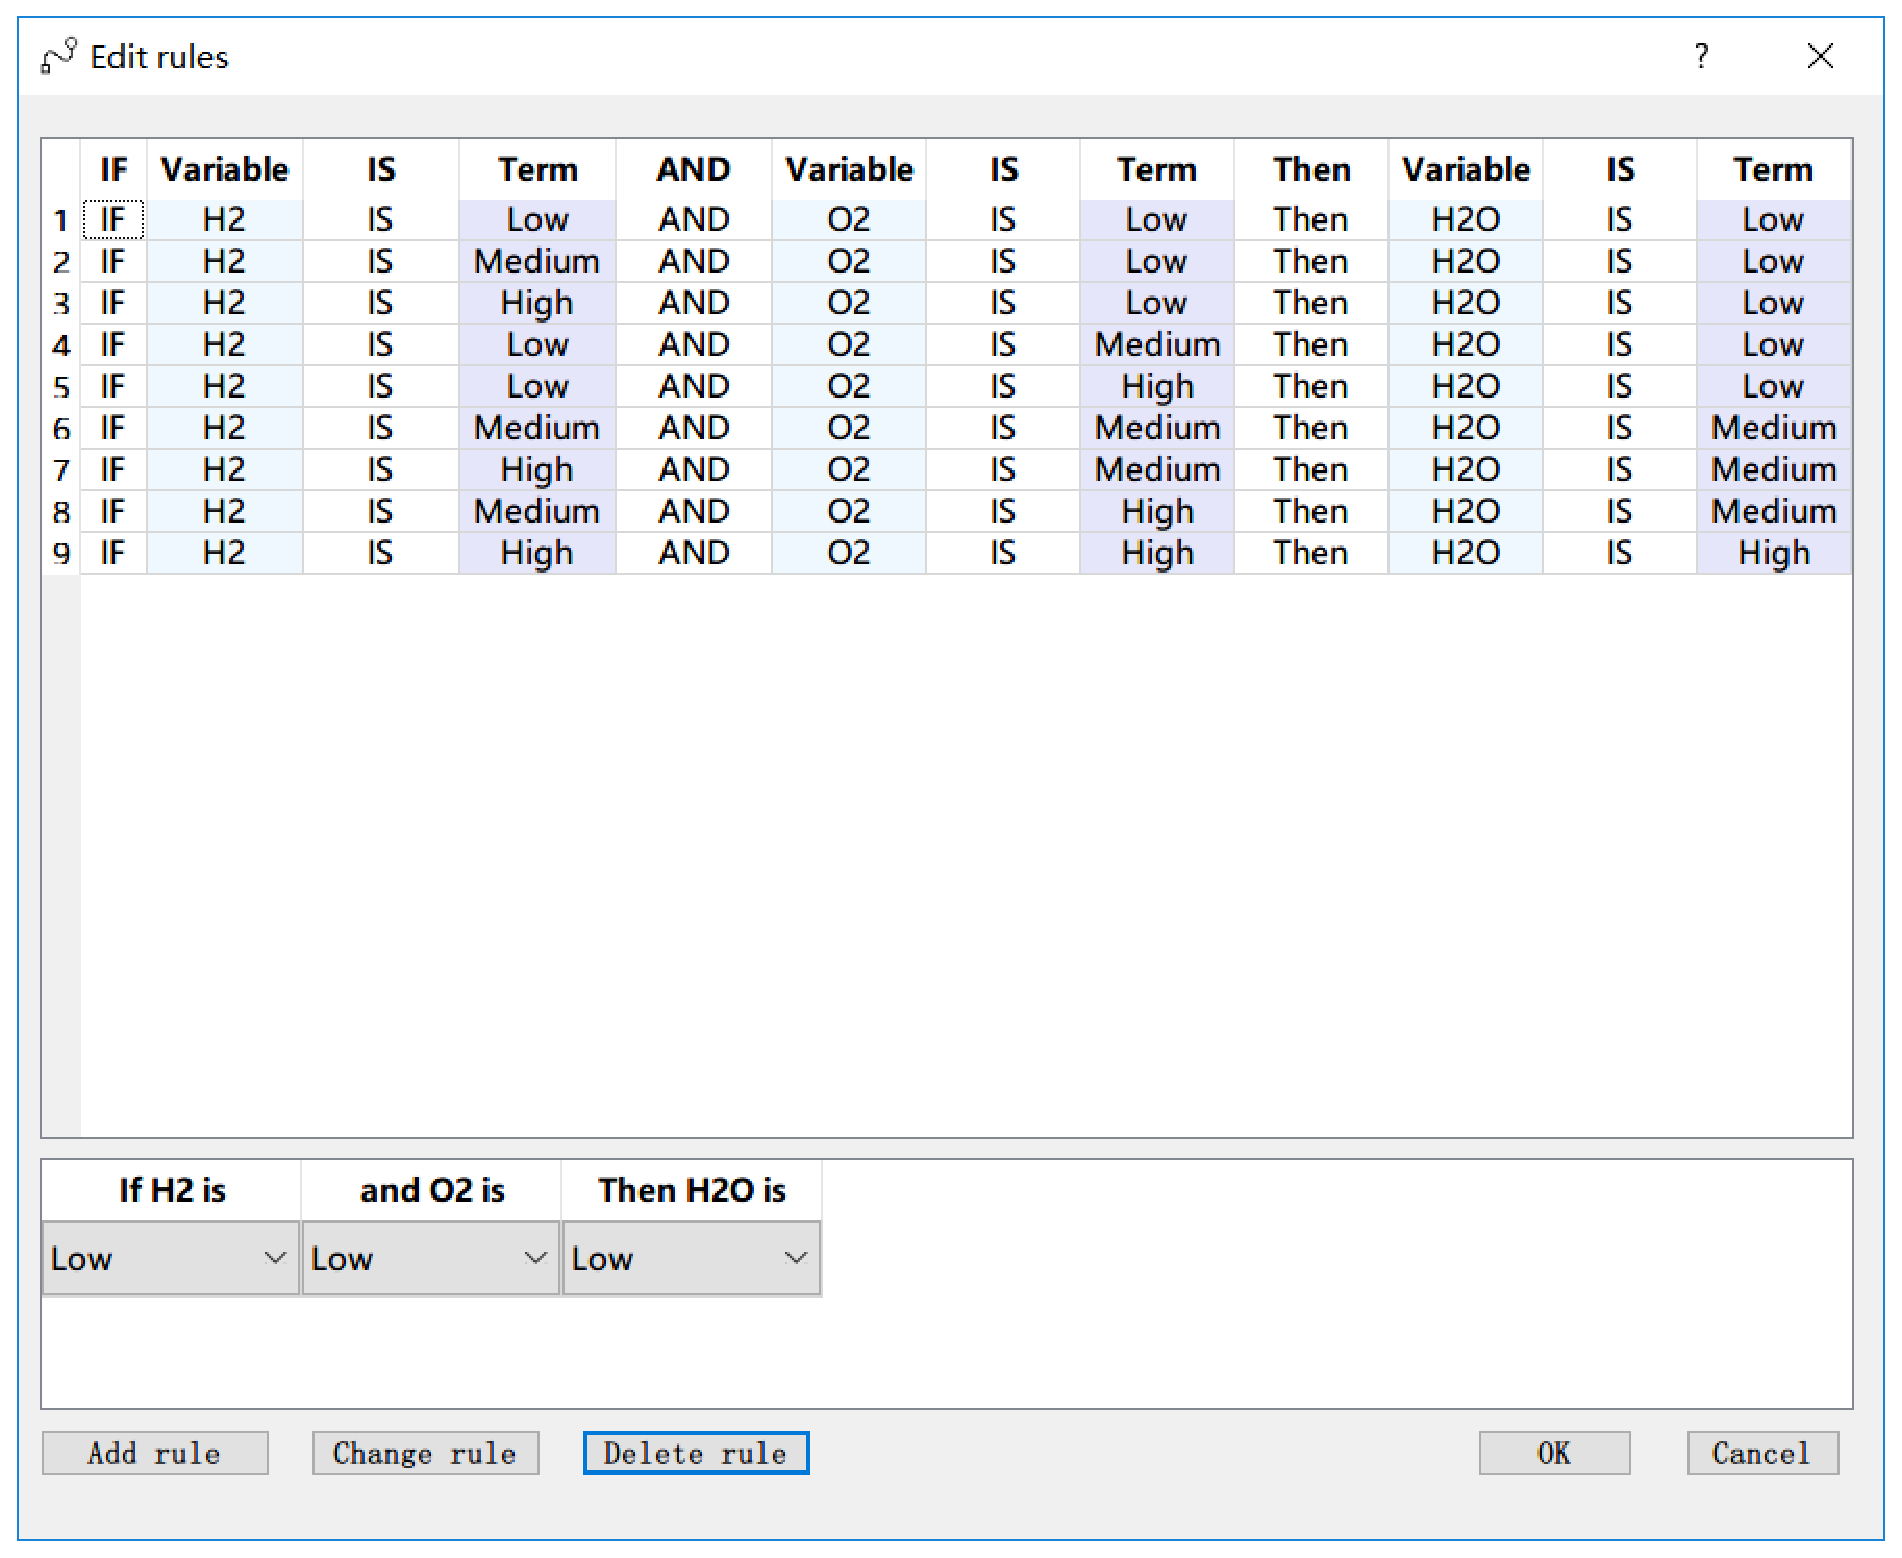
\includegraphics[width=\columnwidth]{fig10}
		\caption{Edit rules.}
		\label{fig:Edit rules}
	\end{center}
\end{figure}

Now left click the OK button of the FIS editor and left click the OK button of the arc to return to the main interface. The net should be like Figure \ref{fig:After FIS}.

\begin{figure}[!hbt]
	\begin{center}
		
\includegraphics[width=\columnwidth]{fig6}
		\caption{The constructed FCPN model with an FIS.}
		\label{fig:After FIS}
	\end{center}
\end{figure}


\clearpage
There are some differences between Mamdani and T-S settings. 

First, in the T-S setting, when left clicking the Edit button of variable whose type is PN\_OUTPUT, there is no need to edit its membership functions.

\begin{figure}[!hbt]
	\begin{center}
		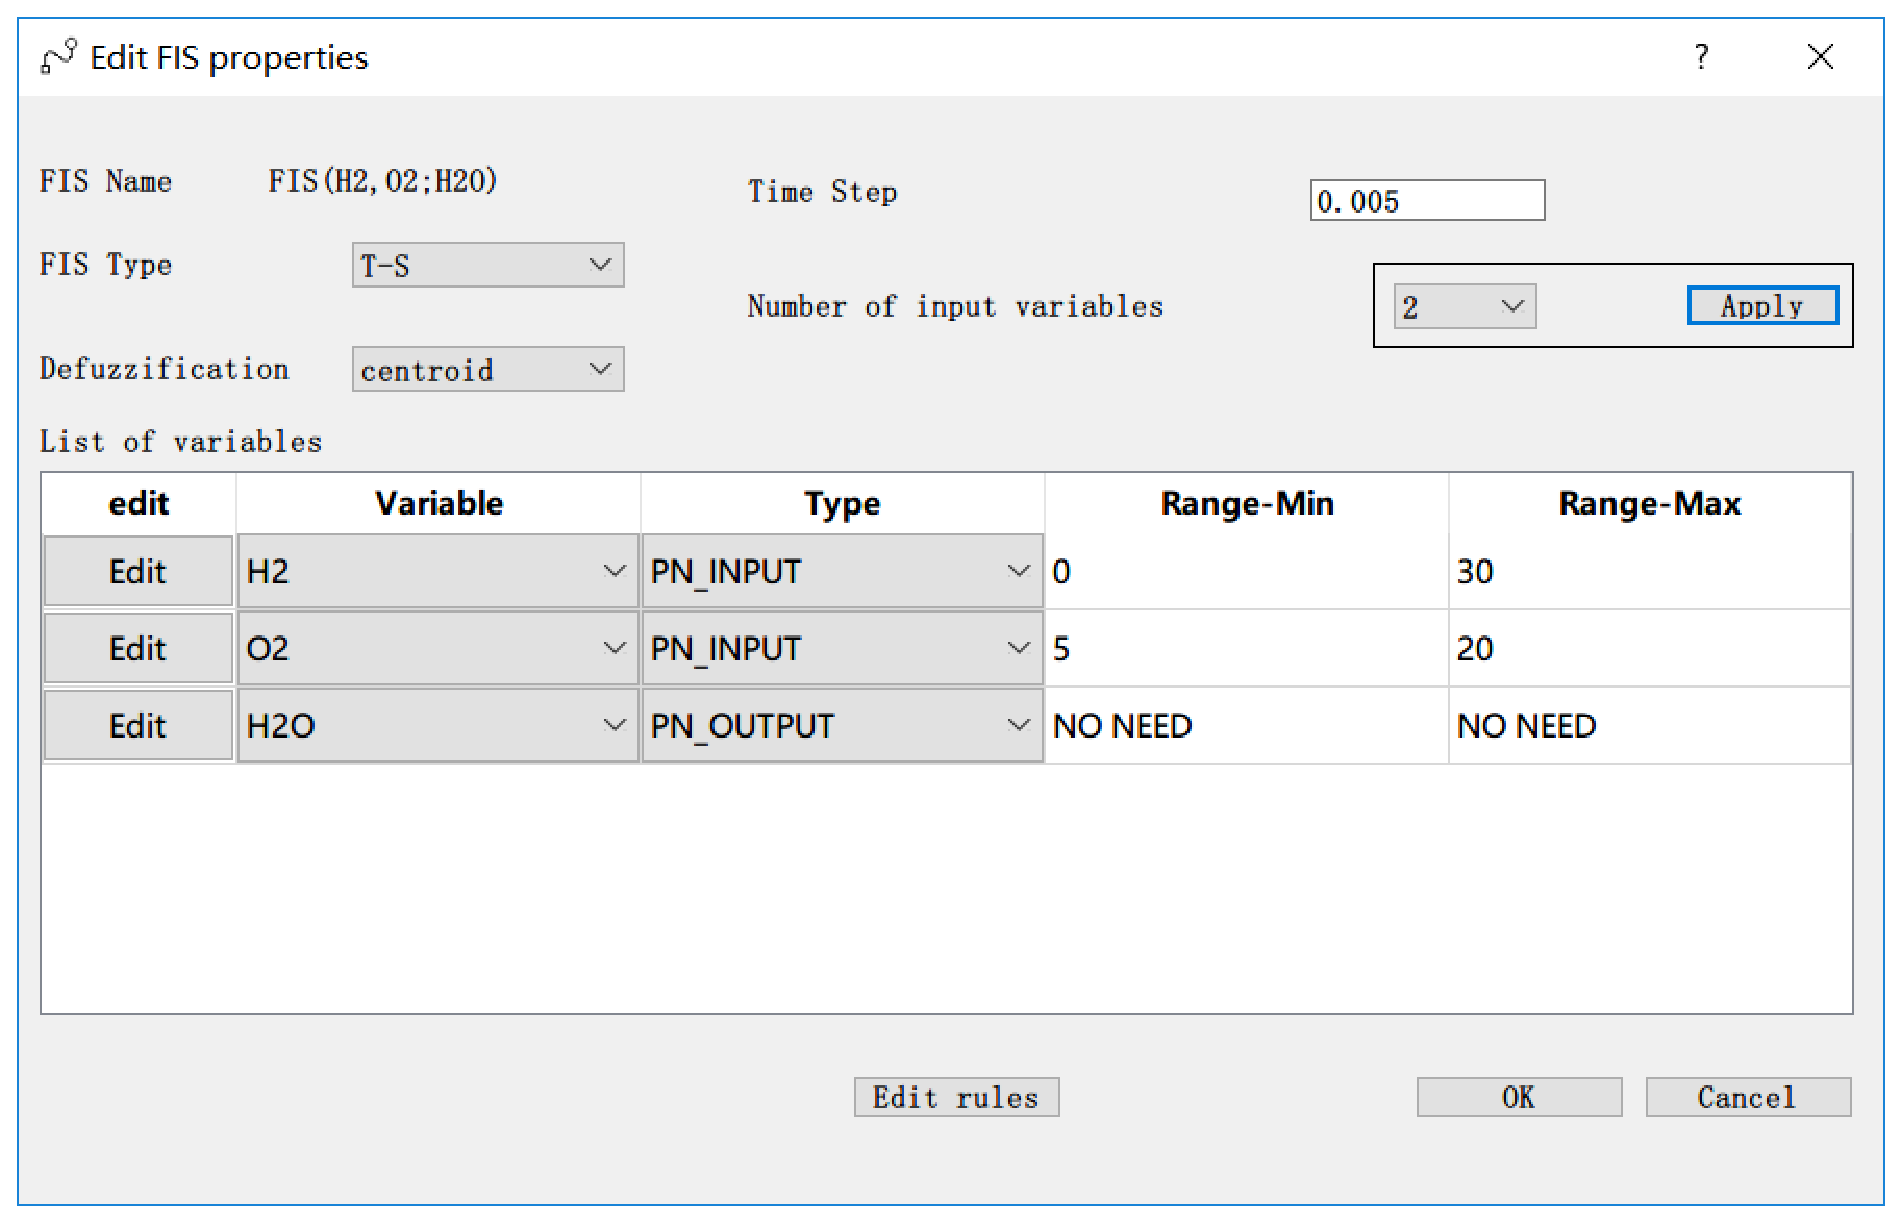
\includegraphics[width=0.8\columnwidth]{fig11}
		\caption{T-S FIS setting.}
		\label{fig:T-S FIS}
	\end{center}
\end{figure}

Second, when editing rules, the last column should be edited by the user as is shown in Figure \ref{fig:Enter rules when using T-S}. 
Add rules first and then change the content of the last column by double clicking the space of the last column of each row and entering the formulas. Then left click the OK button to save changes. 
Other steps are similar to the Mamdani setting.

\begin{figure}[!hbt]
	\begin{center}
		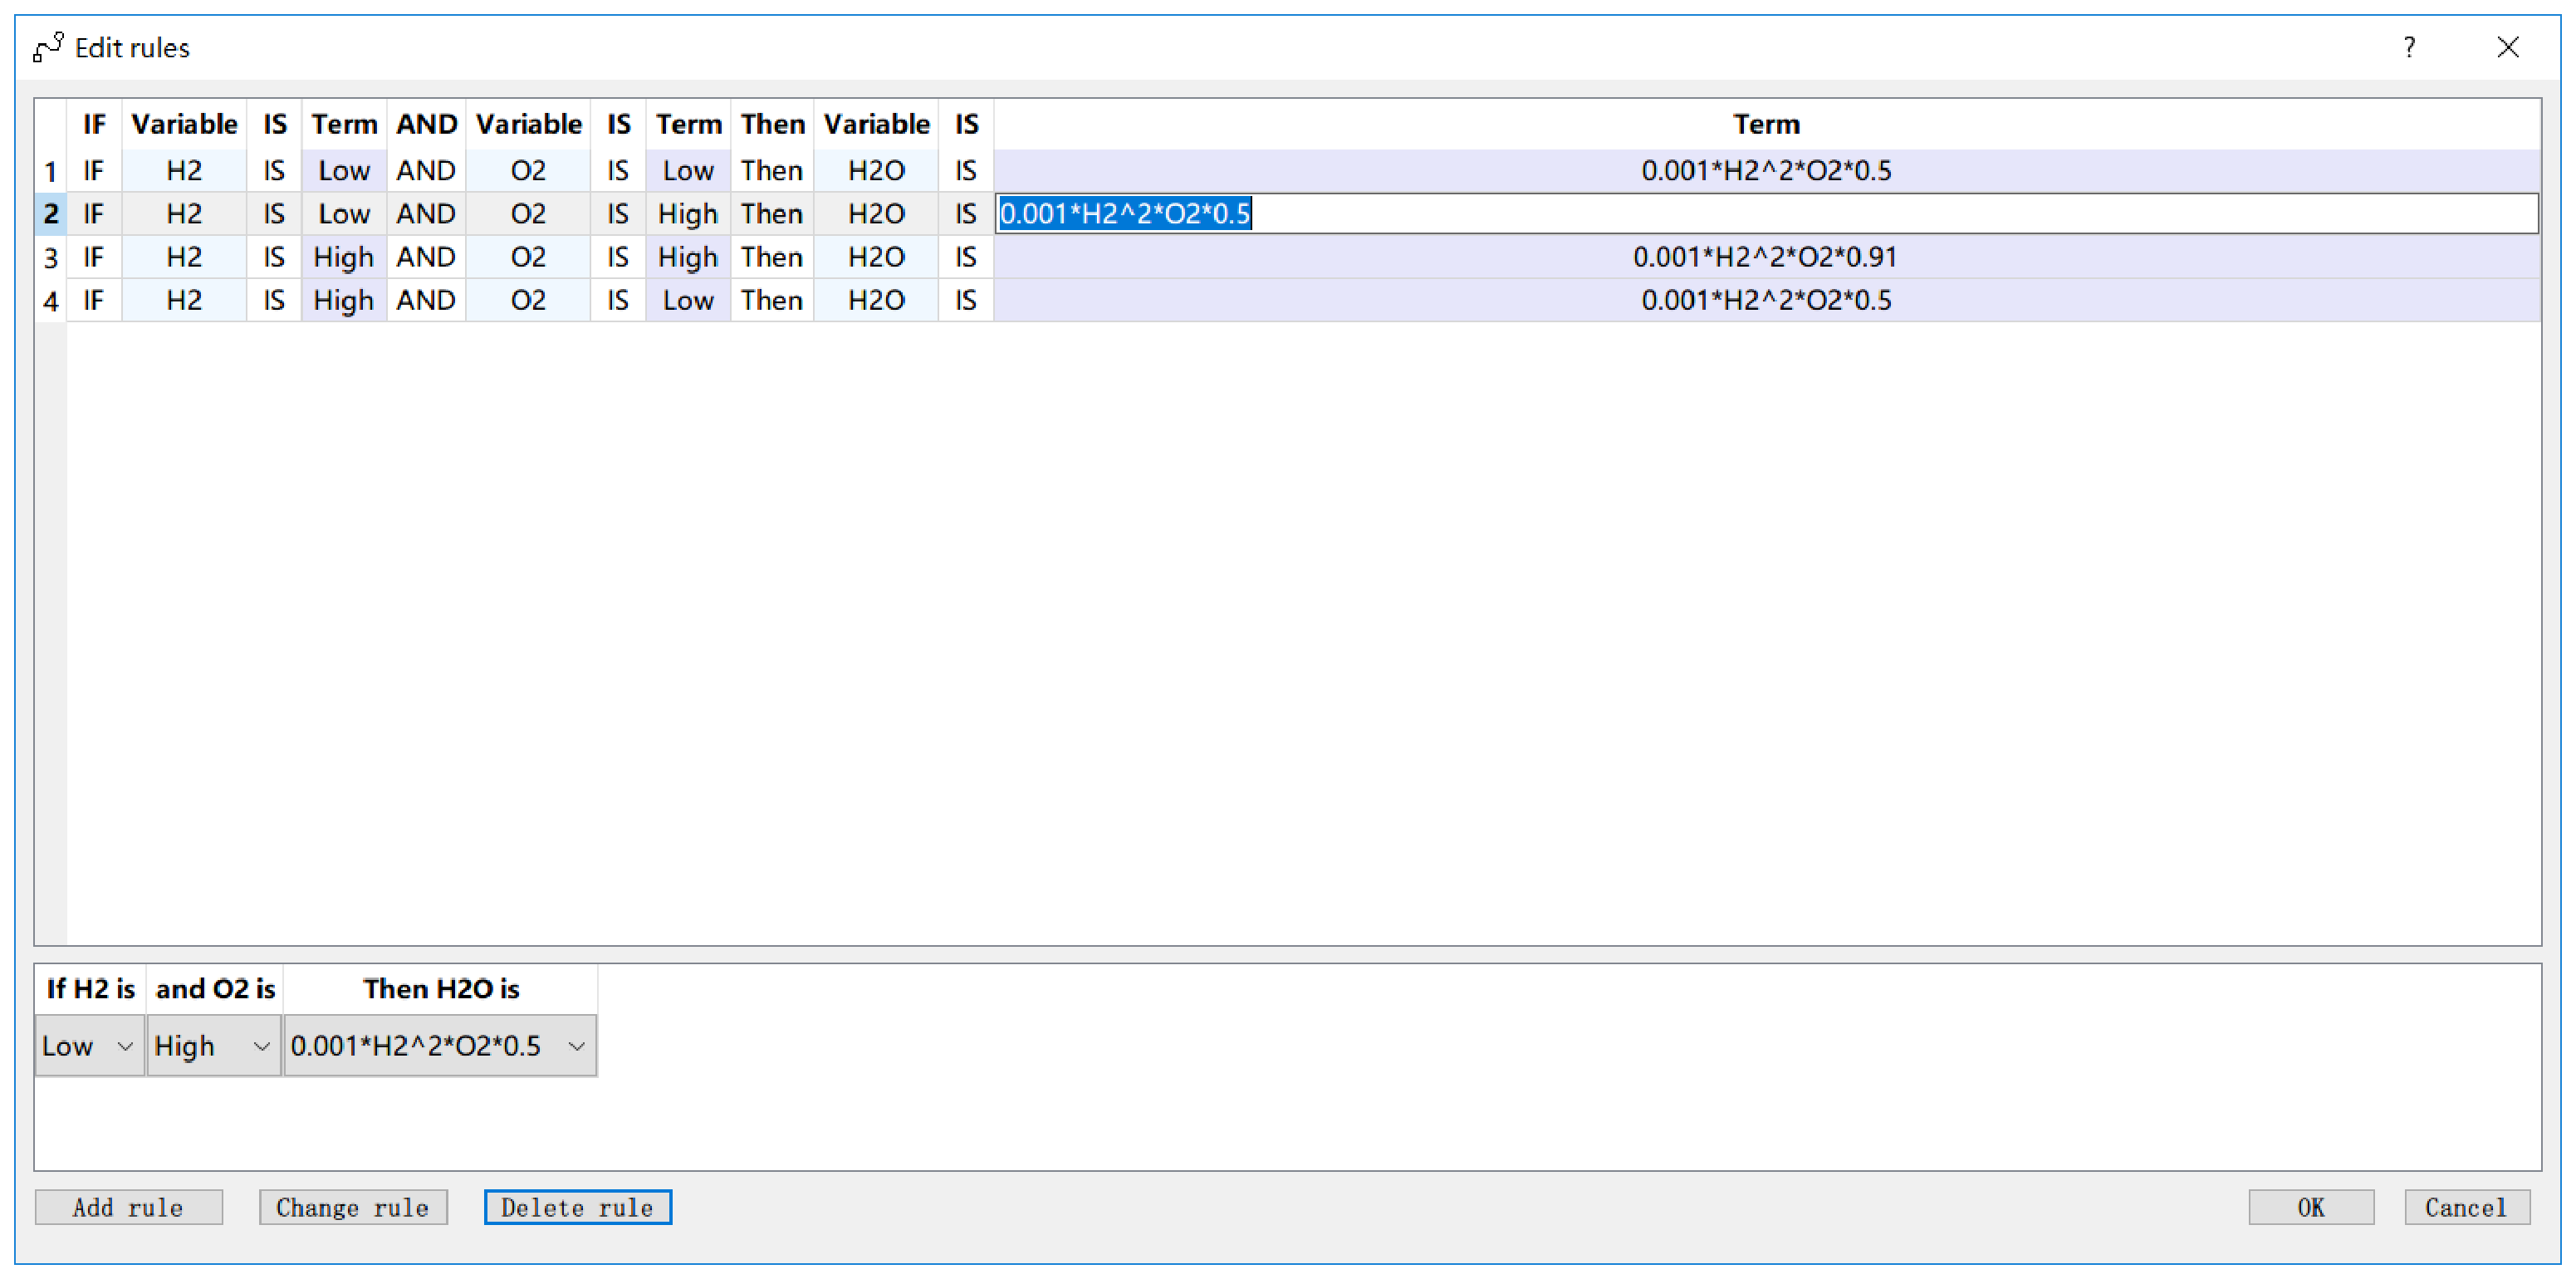
\includegraphics[width=\columnwidth]{fig12}
		\caption{Enter rules when using T-S.}
		\label{fig:Enter rules when using T-S}
	\end{center}
\end{figure}


\clearpage

\section{Simulation}
After an FCPN is finished, left click the ``start simulation'' button on the tool bar to start the simulation function.

\subsection{Run simulation}
In the simulation dialogue shown in Figure \ref{fig:Simulation}, the user can first set simulation parameters, then left click the Start Simulation button to start a simulation. The settings include:
\begin{itemize}
	\item Setting an interval start.
	\item Setting an interval start.
	\item Choosing an ODE solver (only one solver supported at present).
	\item Setting a time step.
	\item Choosing to check negative value or not.
\end{itemize}

Please make sure the time step is smaller than the step size given in the FIS setting. Otherwise the result might be incorrect.

\begin{figure}[!hbt]
	\begin{center}
		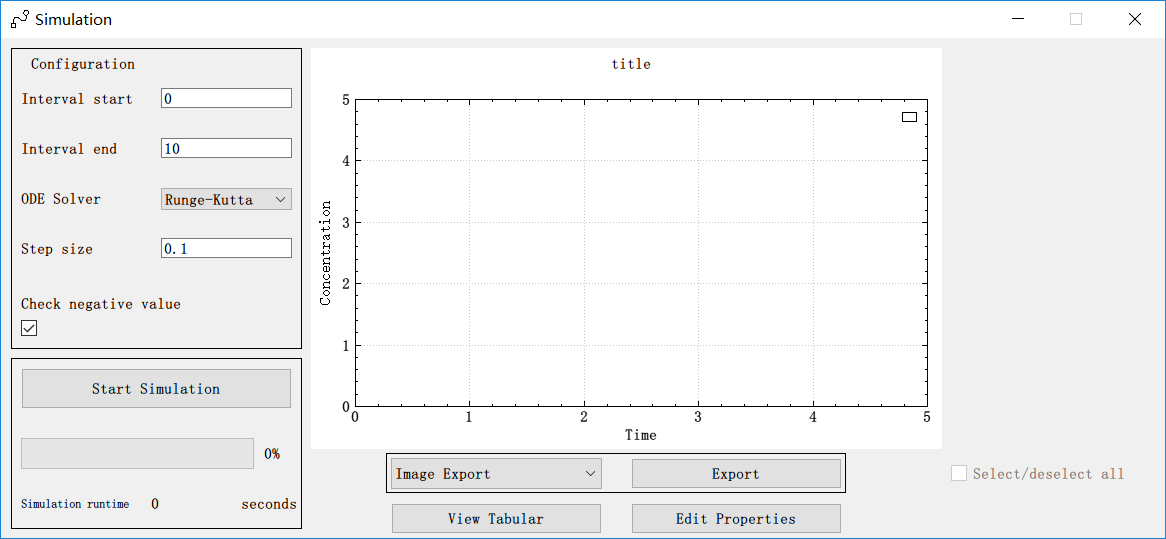
\includegraphics[width=\columnwidth]{fig13}
		\caption{Simulation.}
		\label{fig:Simulation}
	\end{center}
\end{figure}

\subsection{Show simulation results}
During simulation, the progress bar shows the progress of a simulation. After simulation, the plot will show. The user can zoom in or zoom out to see the details and check or uncheck the boxes on the right to show or hide the according variables.

\begin{figure}[!hbt]
	\begin{center}
		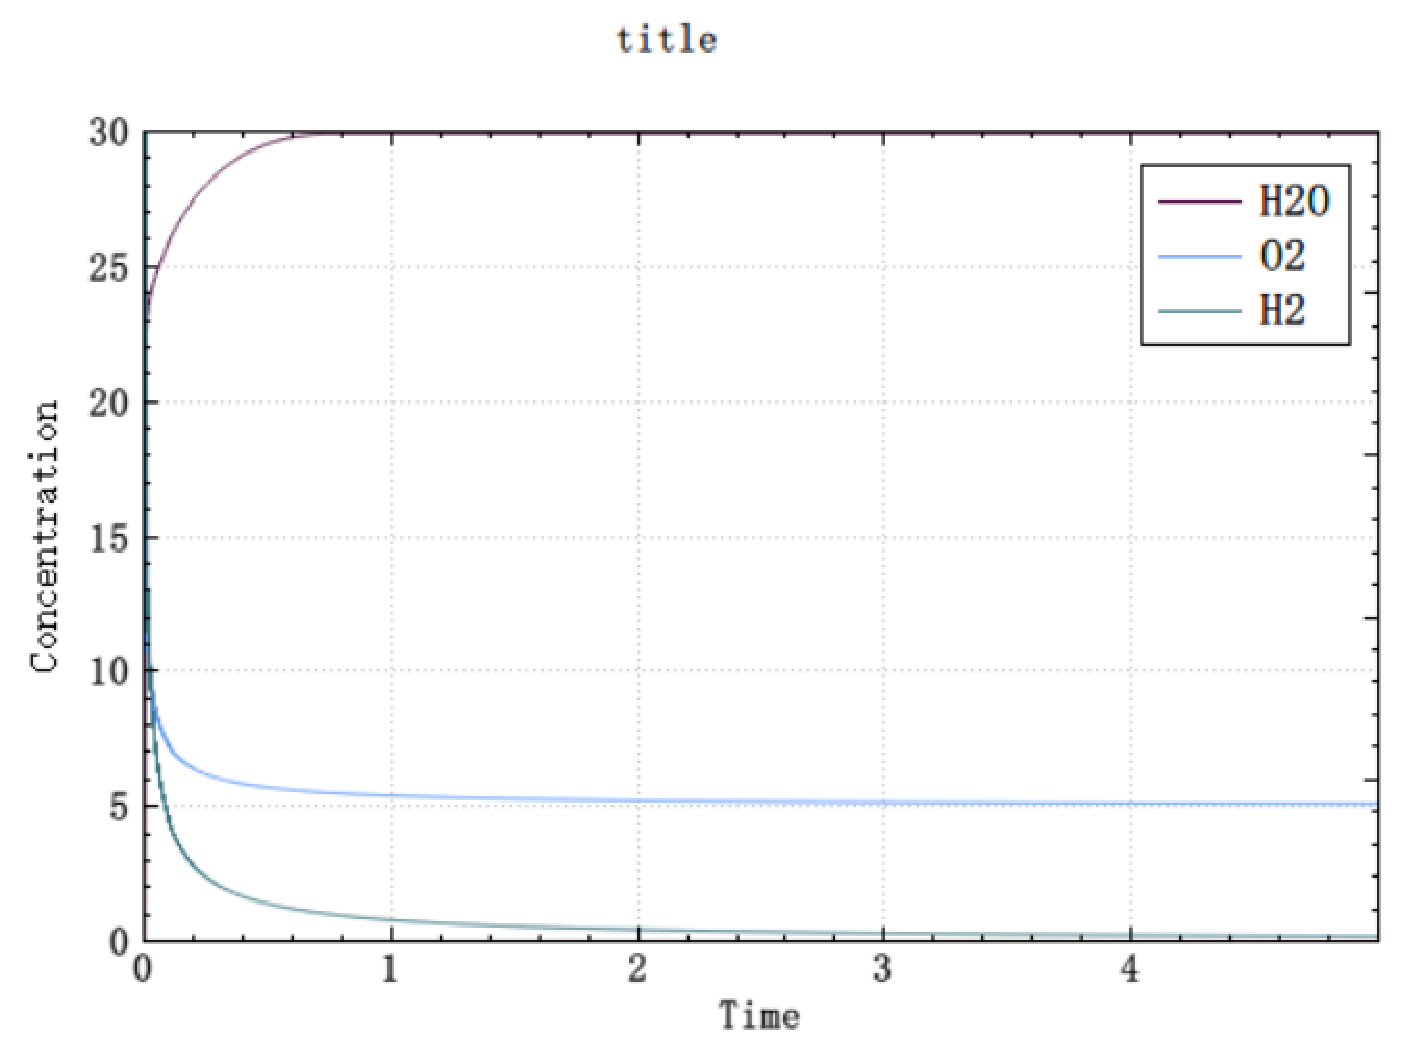
\includegraphics[width=\columnwidth]{fig14}
		\caption{Simulation result (Mamdani).}
		\label{fig:Simulation result (Mamdani)}
	\end{center}
\end{figure}

\begin{figure}[!hbt]
	\begin{center}
		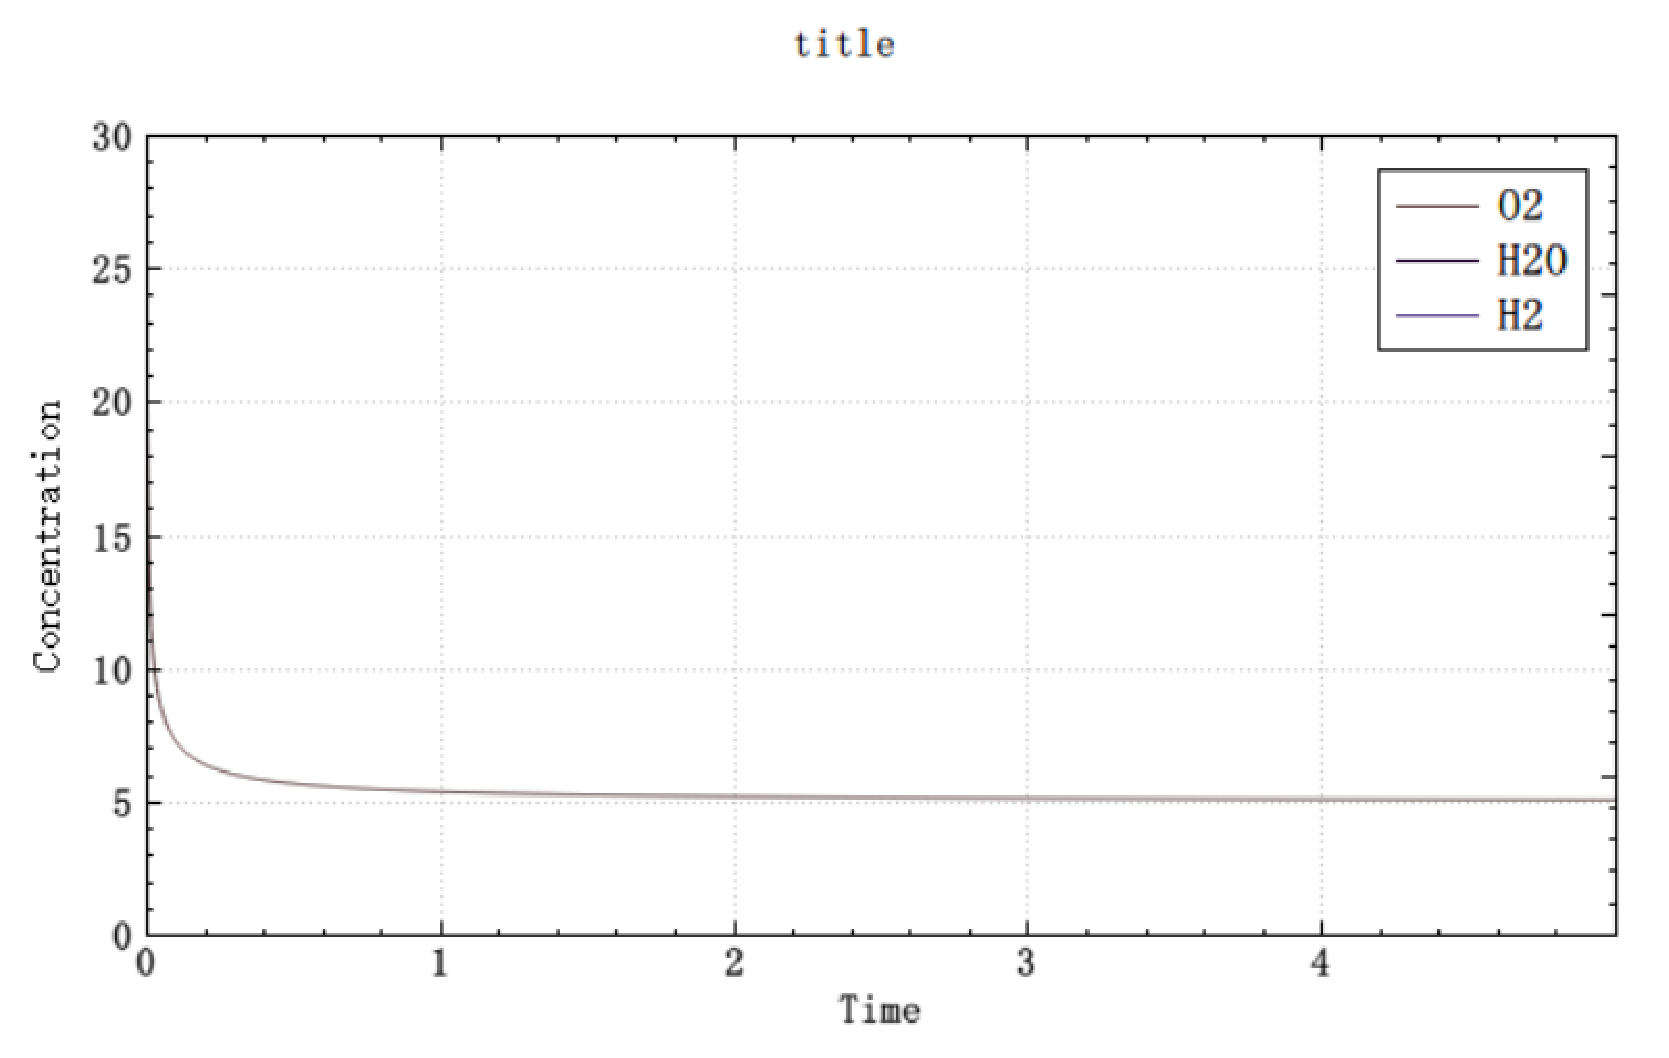
\includegraphics[width=\columnwidth]{fig18}
		\caption{Only show the result of O2.}
		\label{fig:Only show the result of O2}
	\end{center}
\end{figure}

To avoid mis-operation, after entering the simulation, most of the functions in the main interface such as adding items, can not be used. So if you want to get back to edit in the main interface, remember to left click ``normal cursor'' on the left tool bar. Otherwise you will find that most of the functions can't use.

Actually, the user can choose four modes: no FIS, Mamdani, T-S, and hybrid FIS, to run the simulation. Therefore, let us use the no FIS mode to show how to run the simulation. 

\begin{itemize}
	\item Close the simulation window.
	\item Left click ``normal cursor''.
	\item Delete the FIS arc and replace it with a new arc whose expression is 2.
	\item Start simulation again to see the result.
\end{itemize}

The result can be a little bit different, but still shows the general trend.

\begin{figure}[!hbt]
	\begin{center}
		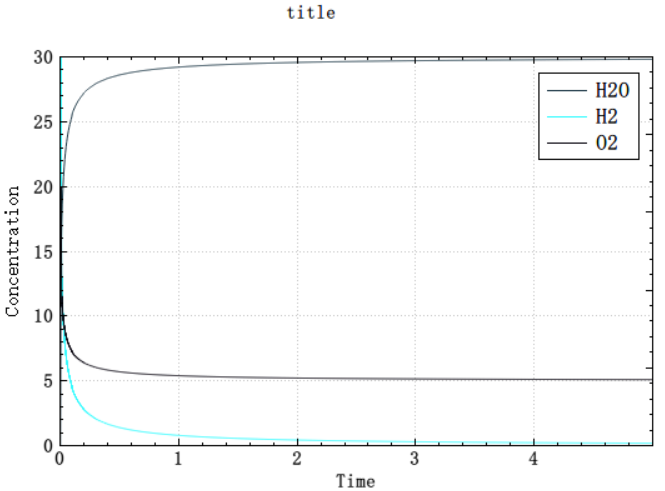
\includegraphics[width=\columnwidth]{fig15}
		\caption{Simulation result (No FIS).}
		\label{fig:Simulation result (No FIS)}
	\end{center}
\end{figure}


\subsection{Export simulation results}
The user can choose the export way and left click the Export button to export.
\begin{figure}[!hbt]
	\begin{center}
		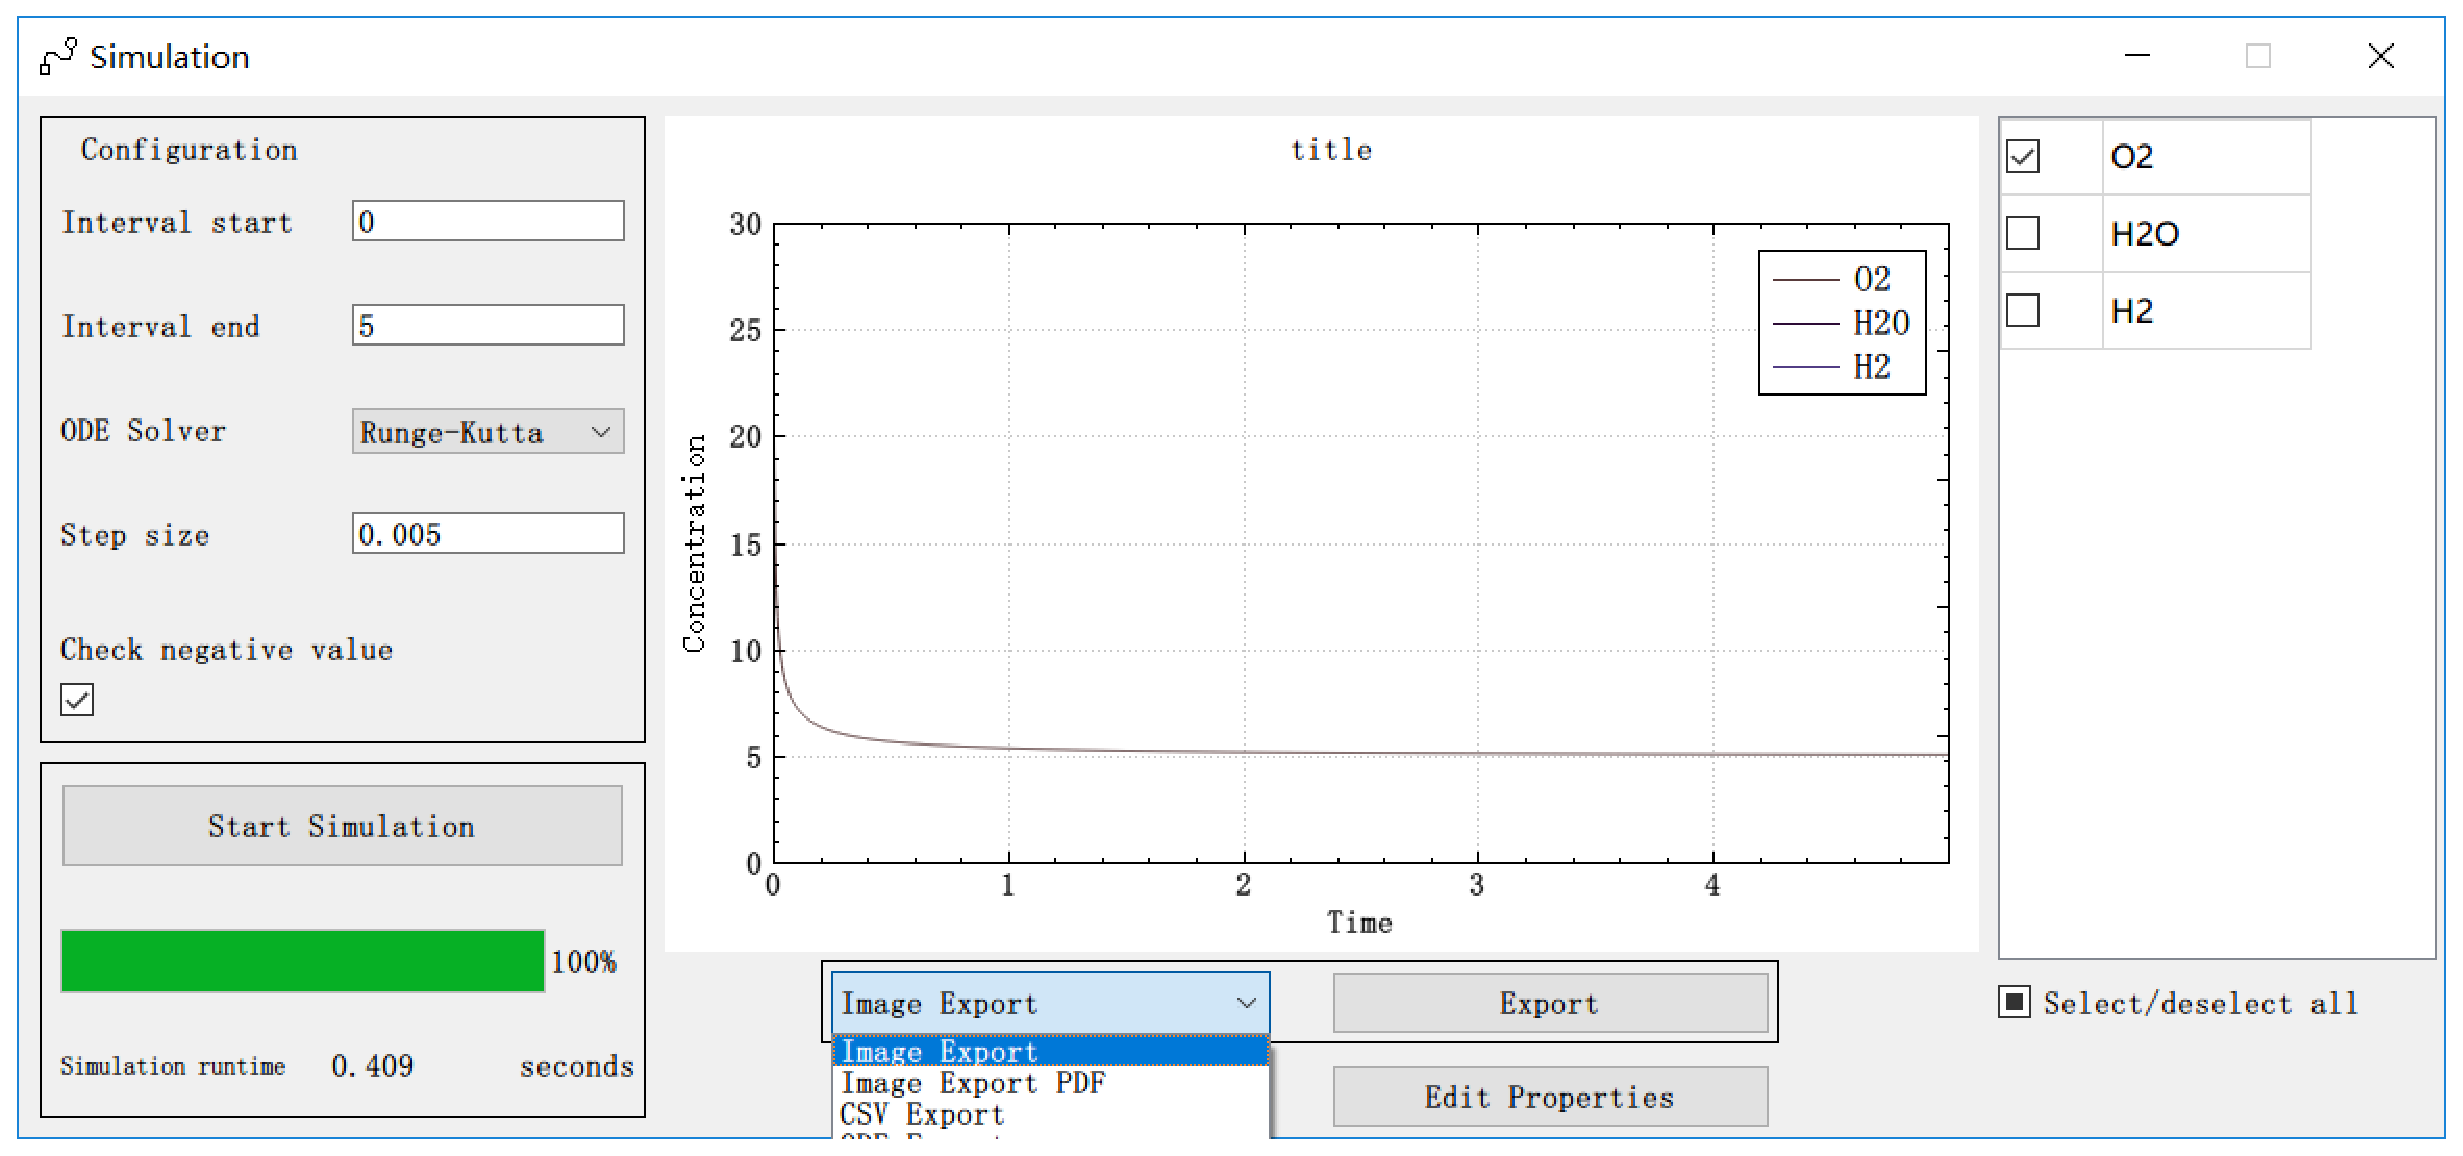
\includegraphics[width=\columnwidth]{fig19}
		\caption{Export result.}
		\label{fig:Export result}
	\end{center}
\end{figure}

\subsection{Rich functions}
Different tools are provided which are located at the center of the bottom. The user can view the Tabular to see the values of variables by left clicking the View Tabular button or edit properties by left clicking the Edit Properties.

\begin{figure}[!hbt]
	\begin{center}
		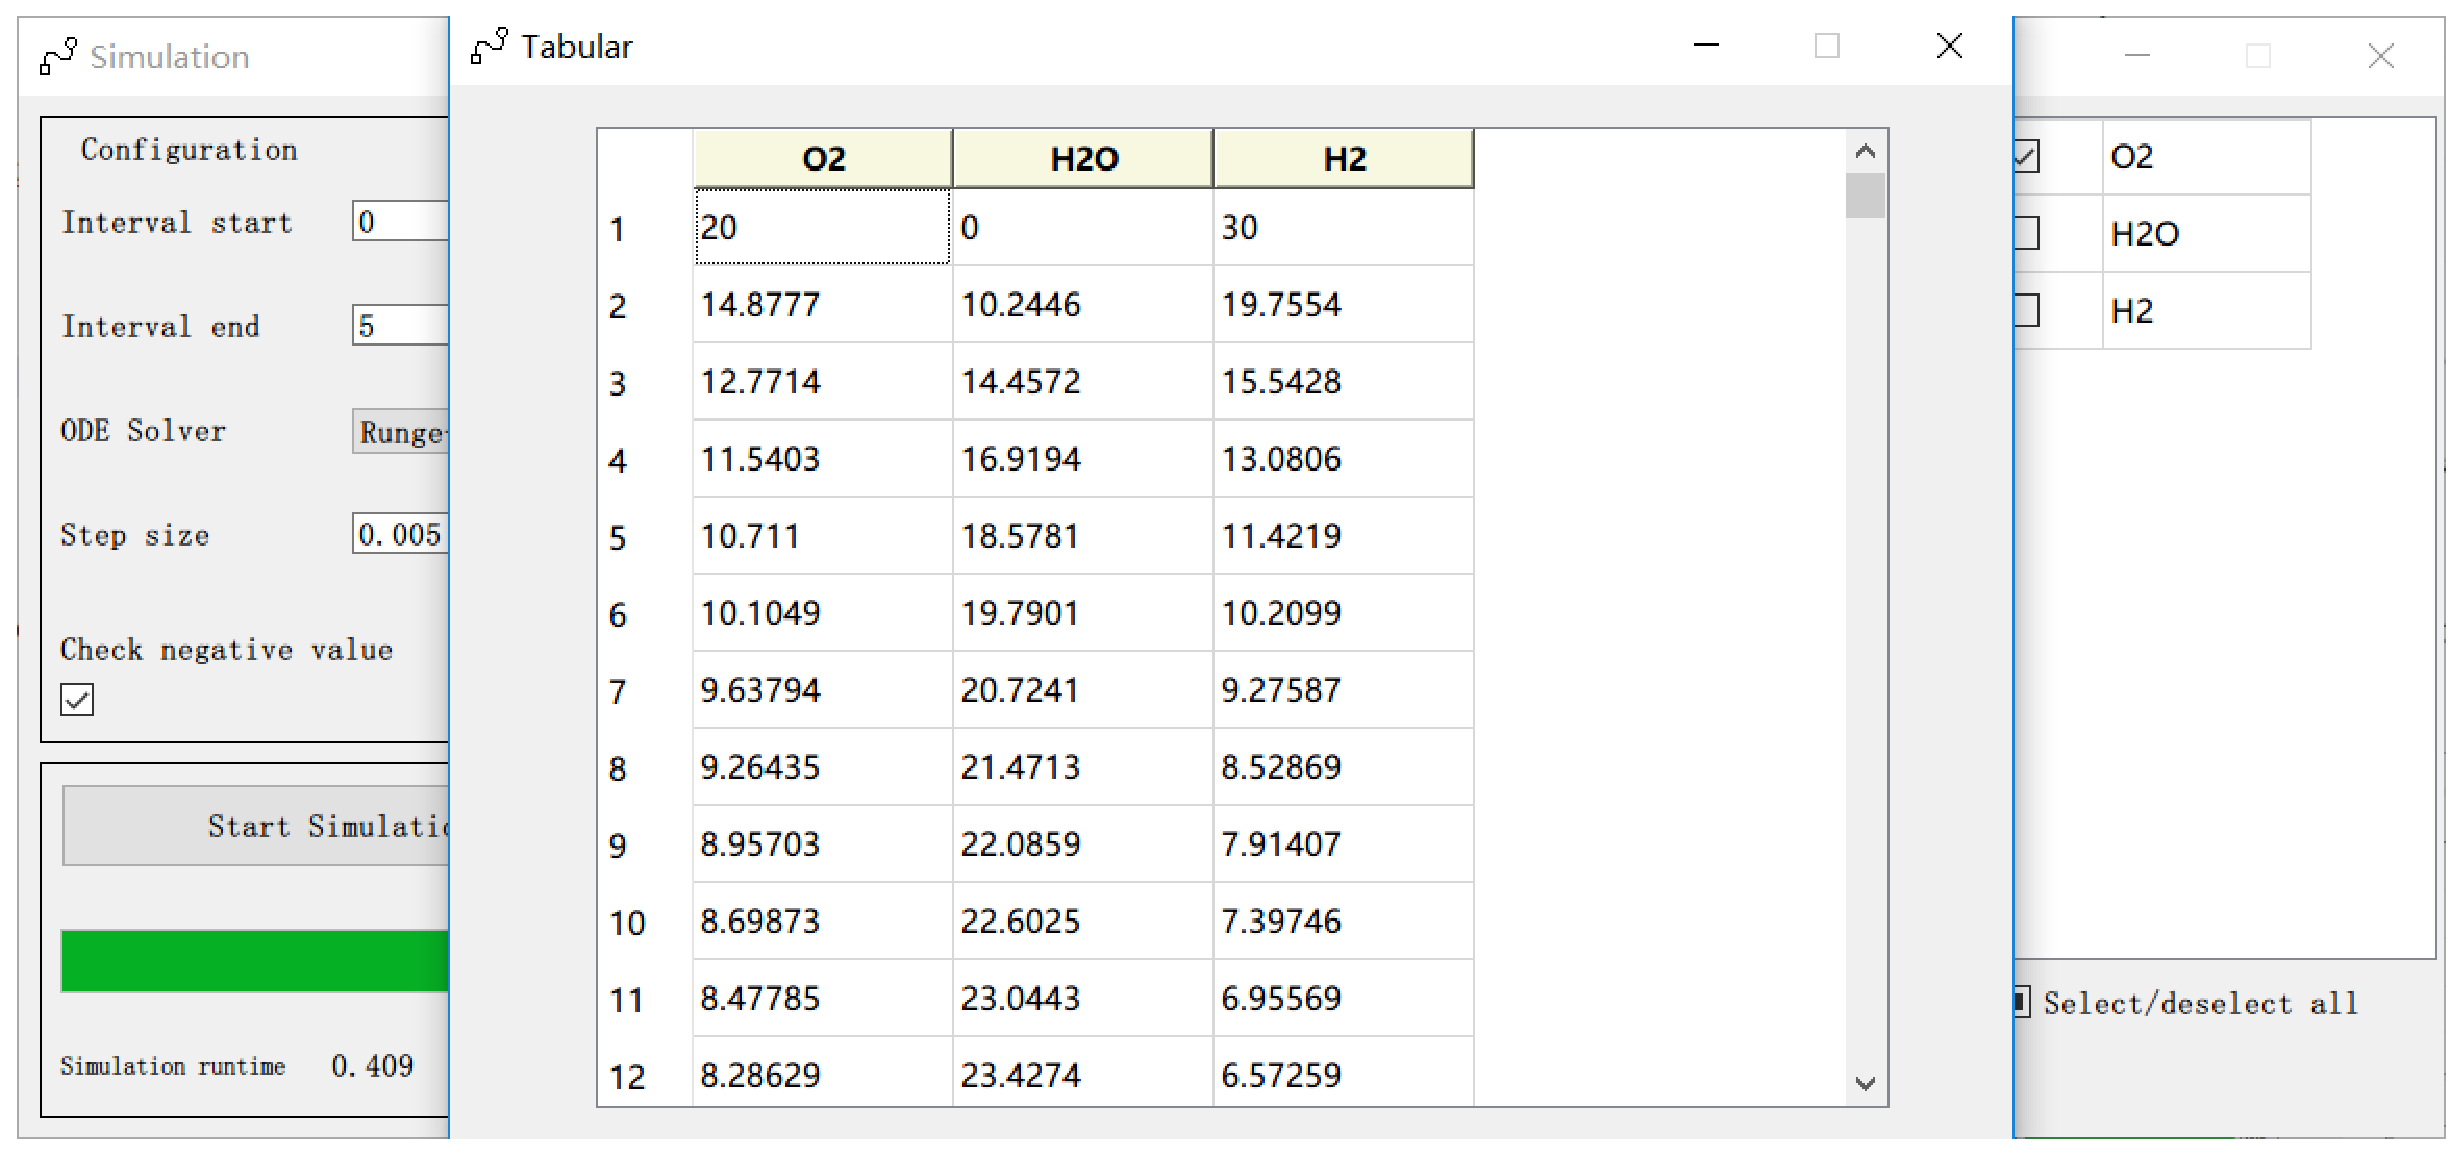
\includegraphics[width=\columnwidth]{fig16}
		\caption{View Tabular.}
		\label{fig:View Tabular}
	\end{center}
\end{figure}

\begin{figure}[!hbt]
	\begin{center}
		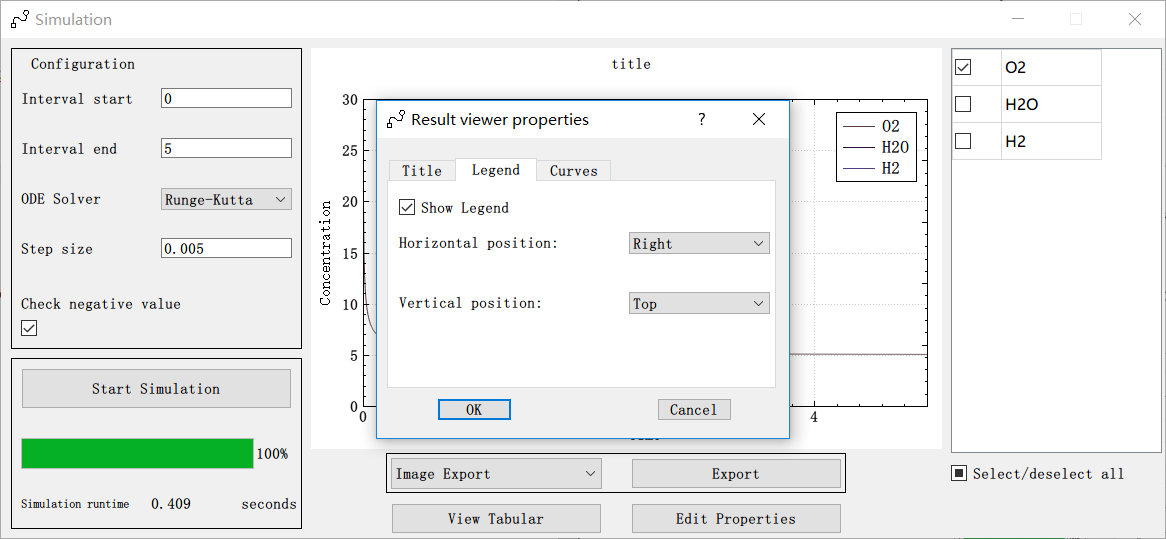
\includegraphics[width=\columnwidth]{fig17}
		\caption{Edit properties.}
		\label{fig:Edit properties.}
	\end{center}
\end{figure}





\clearpage
\section{Examples}
In this section, we will show four examples to illustrate our tool. And we name the file of an example with A\_B\_C\_D, where A is the name of the example, B is the FIS type we used, C is the interval end of the simulation, and D is the step size. The default interval start is 0 for a simulation. 

The models of all the examples can be downloaded from \href{https://github.com/liufei2016/FCPN}{Examples}.


\subsection{1D Diffusion Reaction}

\subsubsection{Introduction}
The first example is one-dimensional (1D) diffusion reaction \cite{LBHY14}, which describes a species diffusing into one of its neighbour cells in a 1D grid.

\subsubsection{Model}
The model is shown in Figure \ref{fig:The model of 1D diffusion reaction}.
\begin{figure}[!hbt]
	\begin{center}
		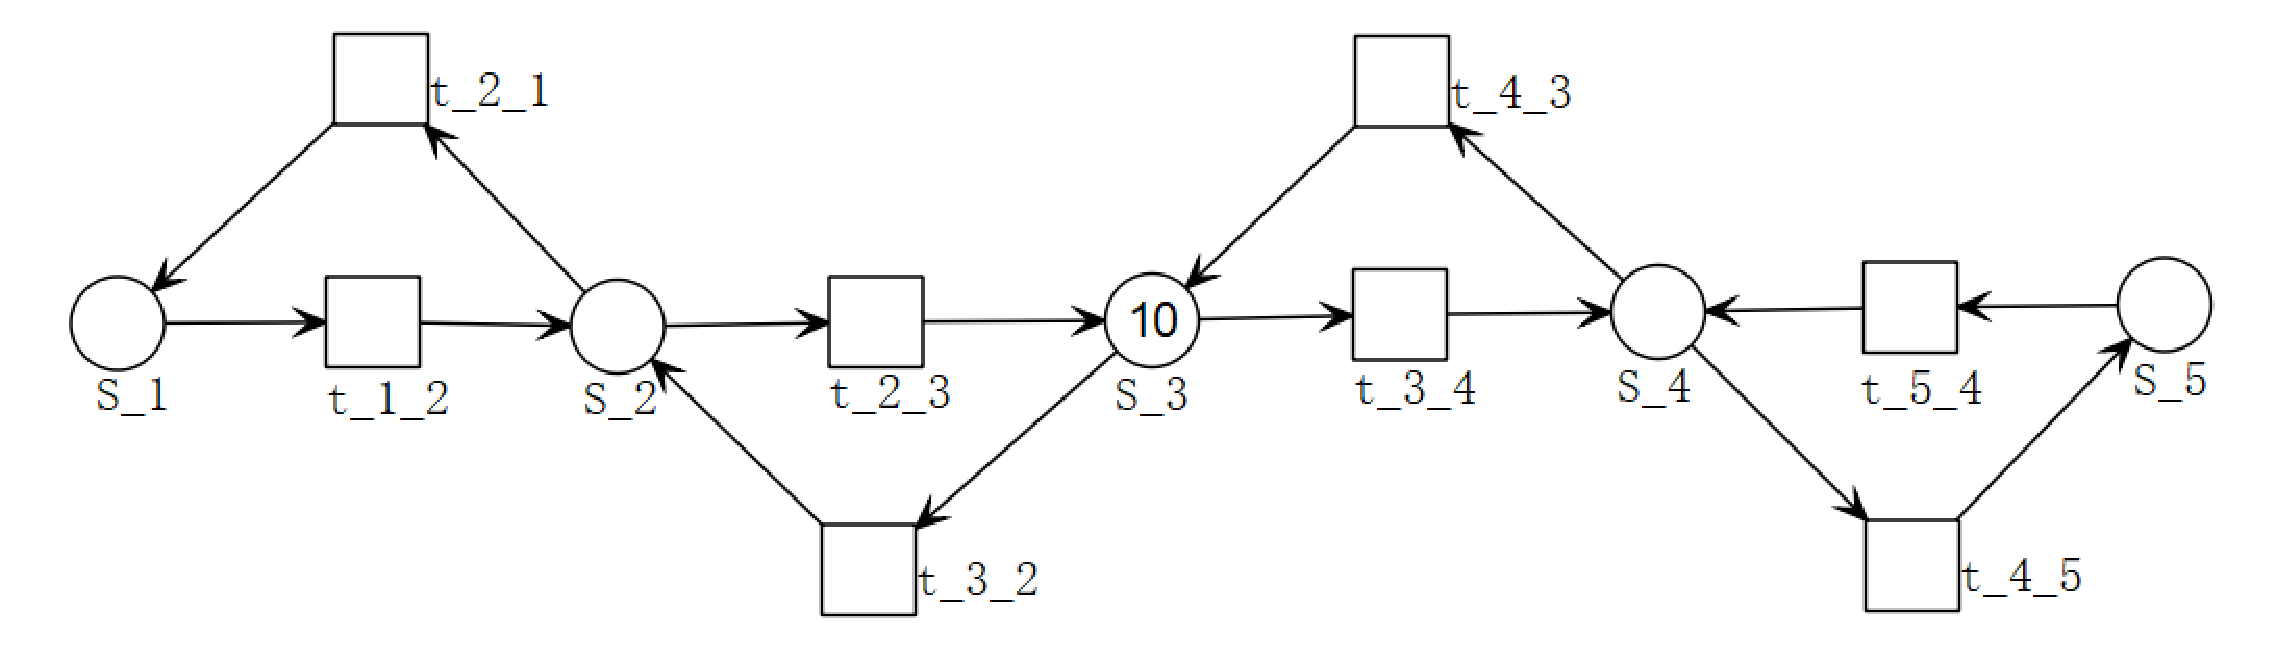
\includegraphics[width=\columnwidth]{fig20}
		\caption{The model of 1D diffusion reaction.}
		\label{fig:The model of 1D diffusion reaction}
	\end{center}
\end{figure}

\begin{table}[!hbt]
	\begin{center}
		\caption{Transition functions of the model of 1D Diffusion Reaction.}
		\label{Transition functions of 1D Diffusion Reaction}
		\begin{tabular}{|c|c|}
			\hline
			Transition&Function\\
			\hline
			t\_1\_2&MassAction(1)\\
			\hline
						t\_2\_1&MassAction(1)\\
			\hline
						t\_2\_3&MassAction(1)\\
			\hline
						t\_3\_2&MassAction(1)\\
			\hline
						t\_3\_4&MassAction(1)\\
			\hline
						t\_4\_3&MassAction(1)\\
			\hline
						t\_4\_5&MassAction(1)\\
			\hline
						t\_5\_4&MassAction(1)\\
			\hline
		\end{tabular}
	\end{center}
\end{table}

\begin{figure}[!hbt]
	\begin{center}
		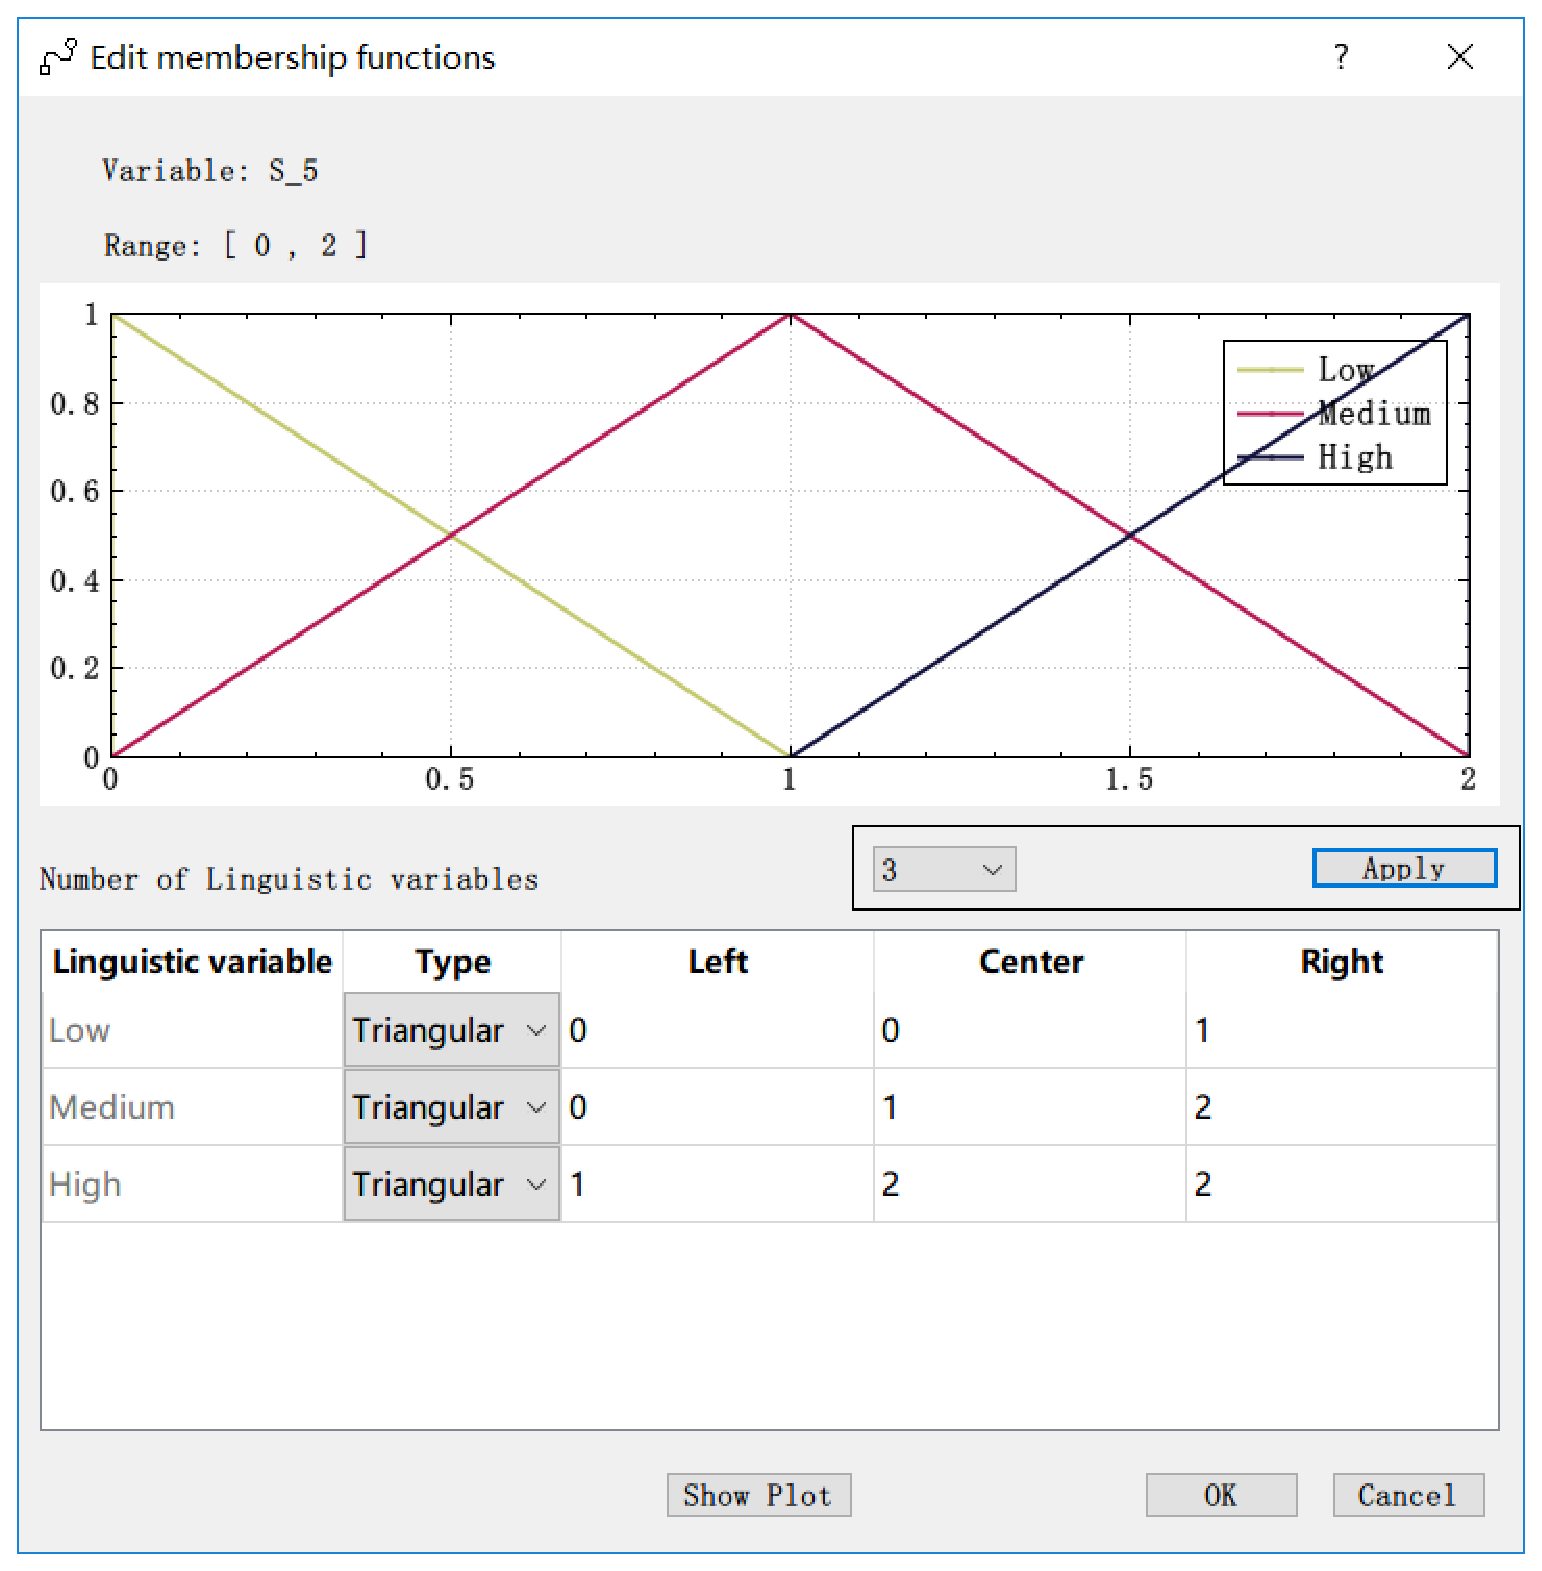
\includegraphics[width=0.45\columnwidth]{fig31}
		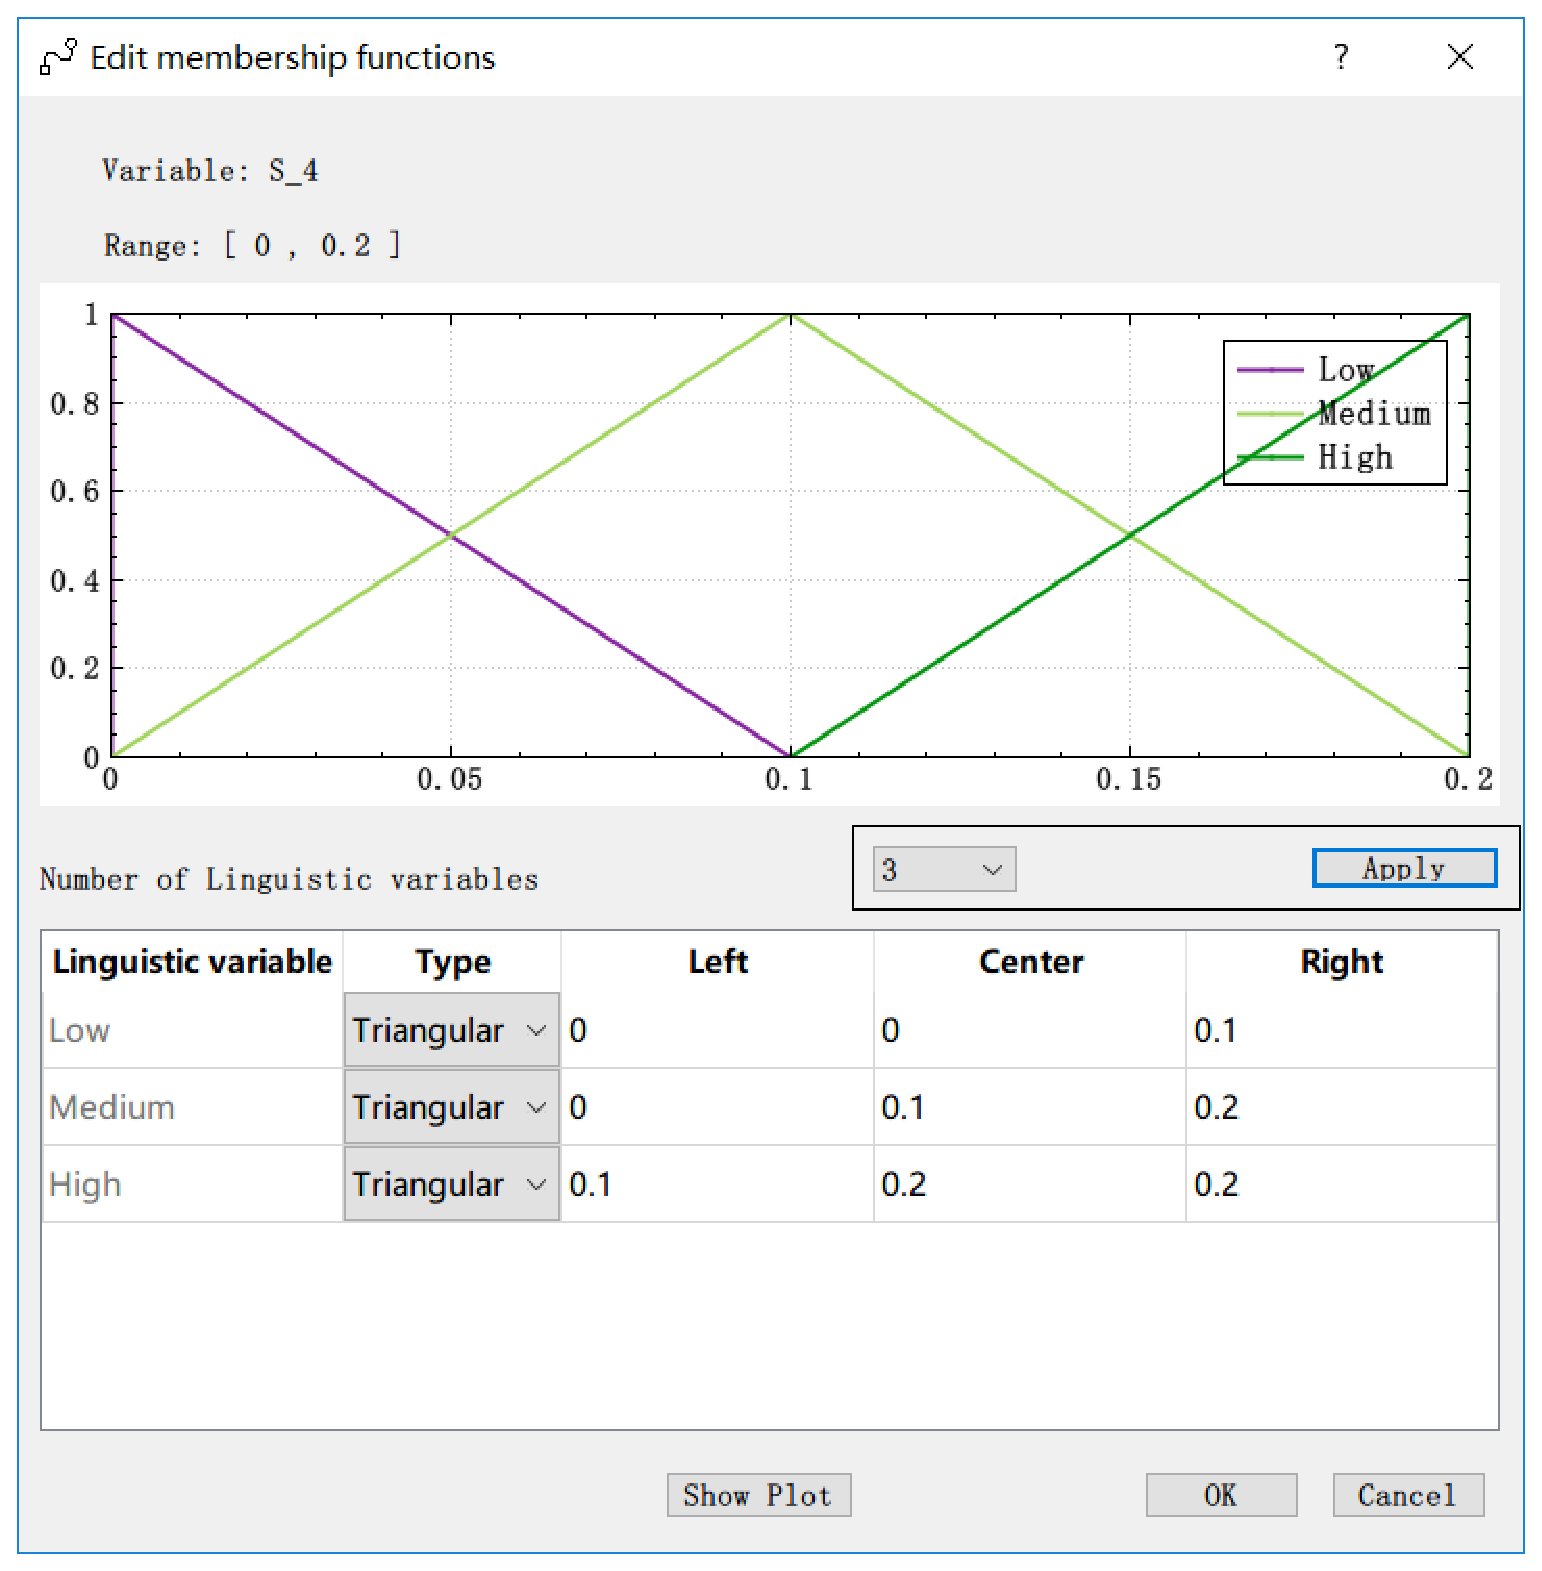
\includegraphics[width=0.45\columnwidth]{fig32}
		\caption{Membership functions of the 1D Diffusion Reaction model using the Mamdani setting.}
		\label{fig:Membership functions of 1D Diffusion Reaction using Mamdani.}
	\end{center}
\end{figure}

\begin{figure}[!hbt]
	\begin{center}
		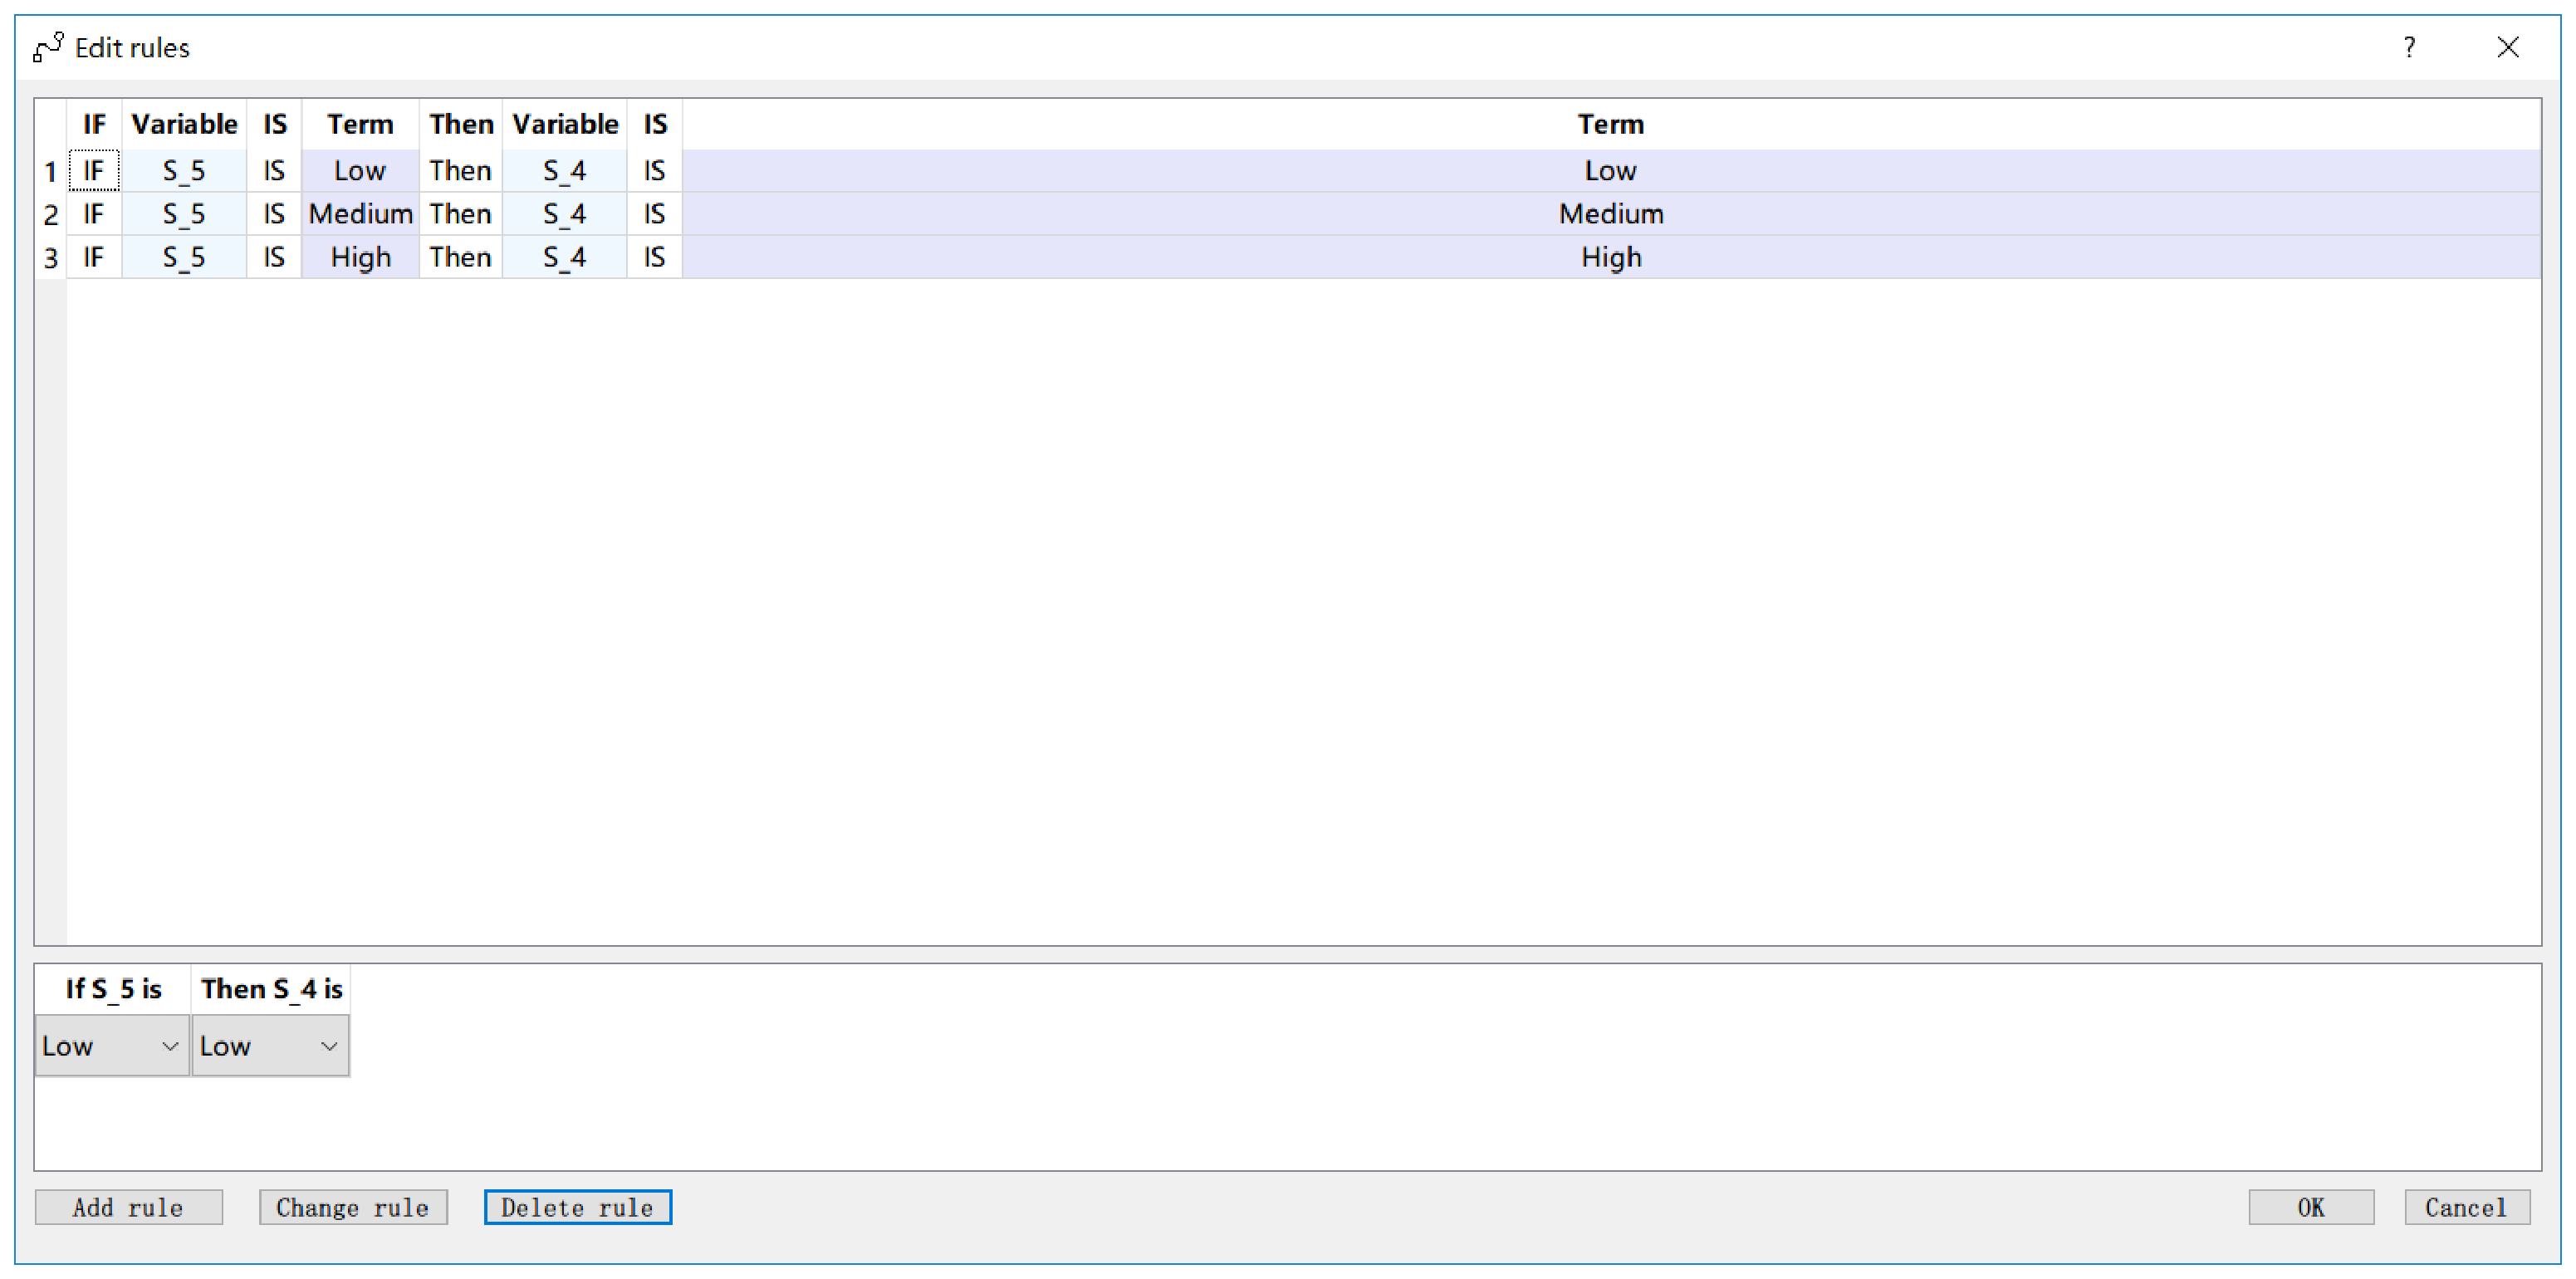
\includegraphics[width=\columnwidth]{fig33}
		\caption{Rules of the 1D Diffusion Reaction model using the Mamdani setting.}
		\label{fig:Rules of 1D Diffusion Reaction using Mamdani.}
	\end{center}
\end{figure}

\begin{figure}[!hbt]
	\begin{center}
		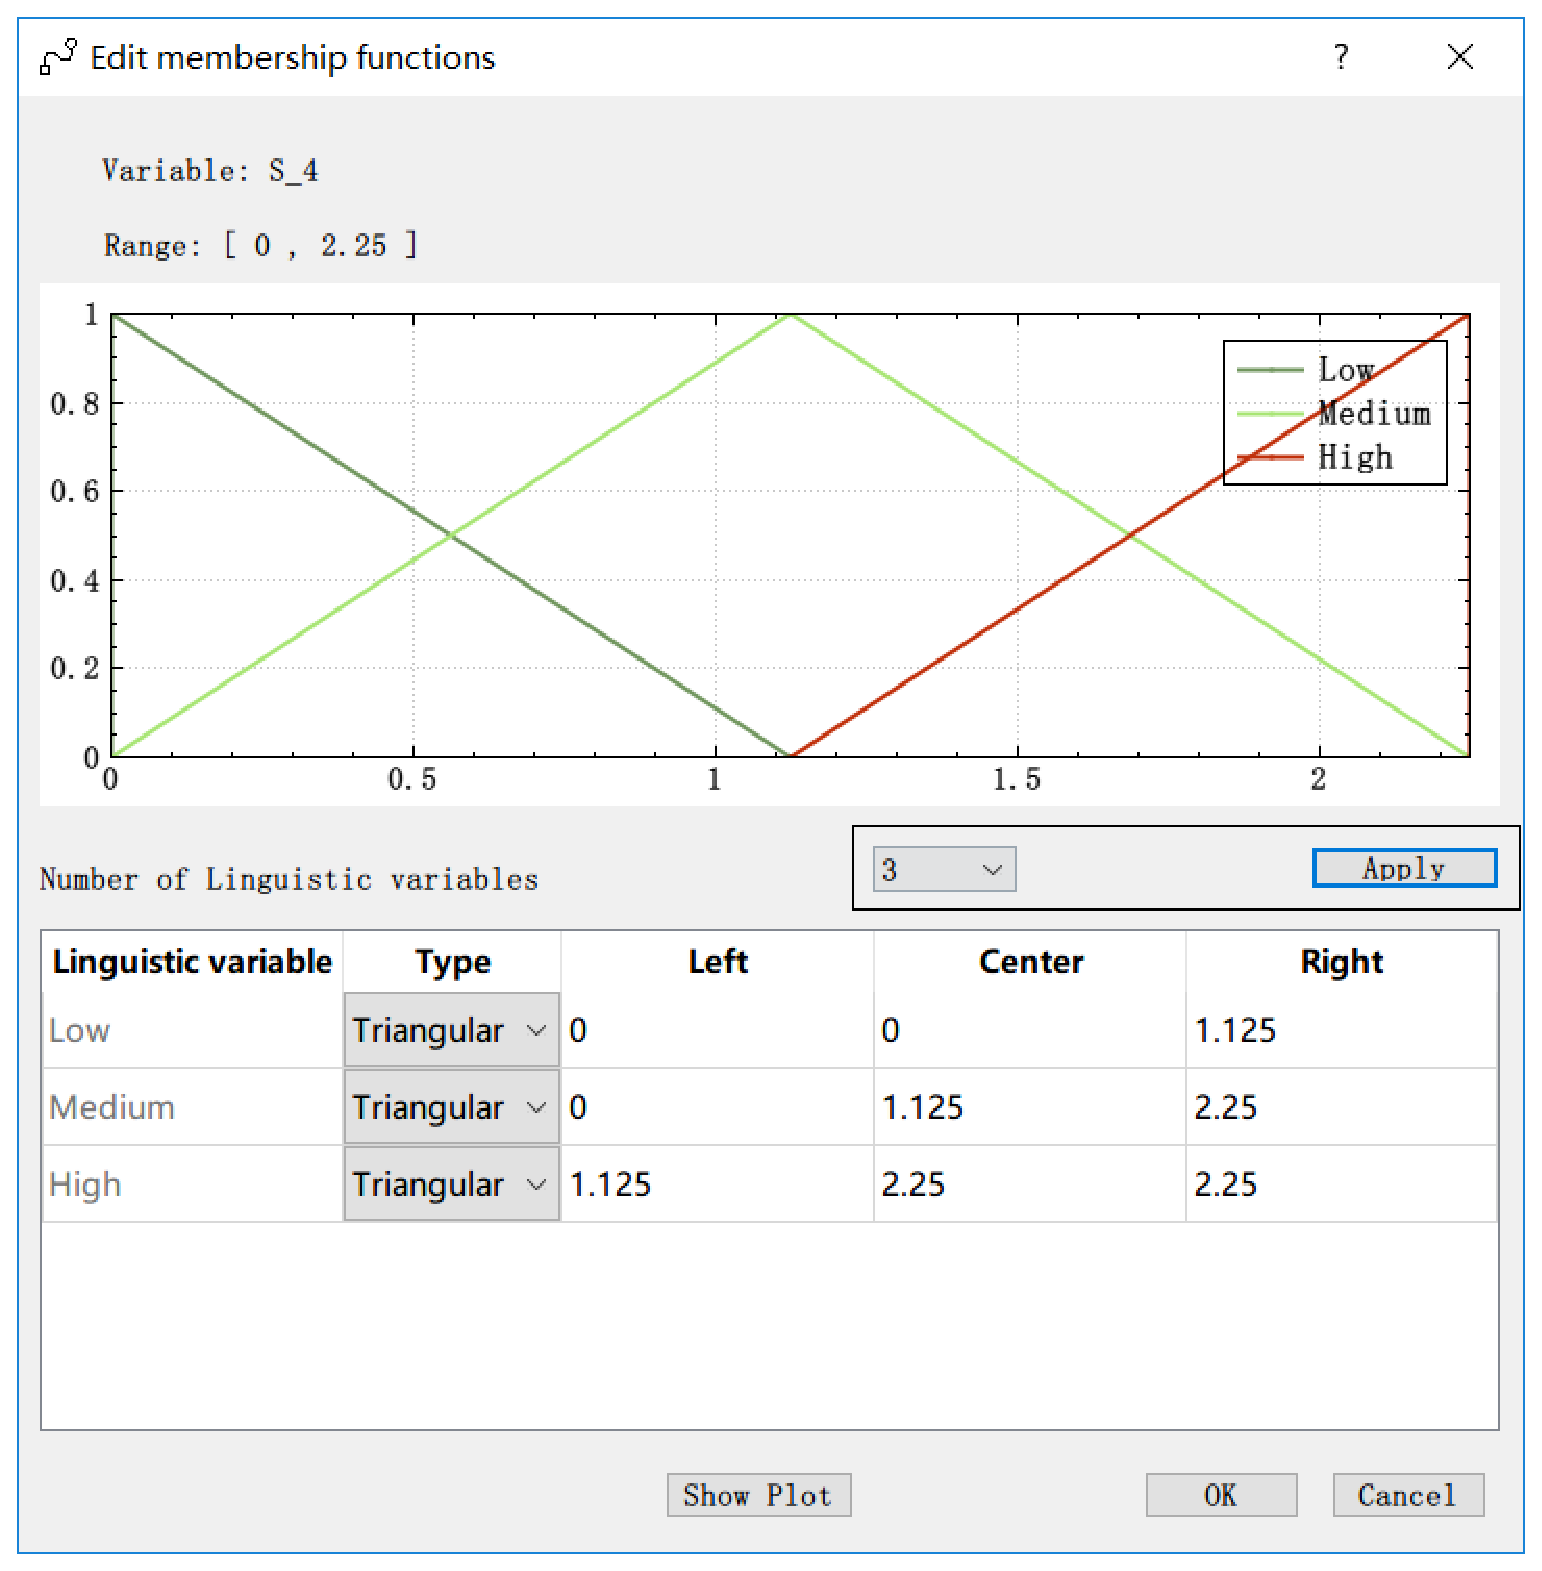
\includegraphics[width=\columnwidth]{fig34}
		\caption{Membership functions of the 1D Diffusion Reaction model using the T-S setting.}
		\label{fig:Membership functions of 1D Diffusion Reaction using T-S.}
	\end{center}
\end{figure}

\begin{figure}[!hbt]
	\begin{center}
		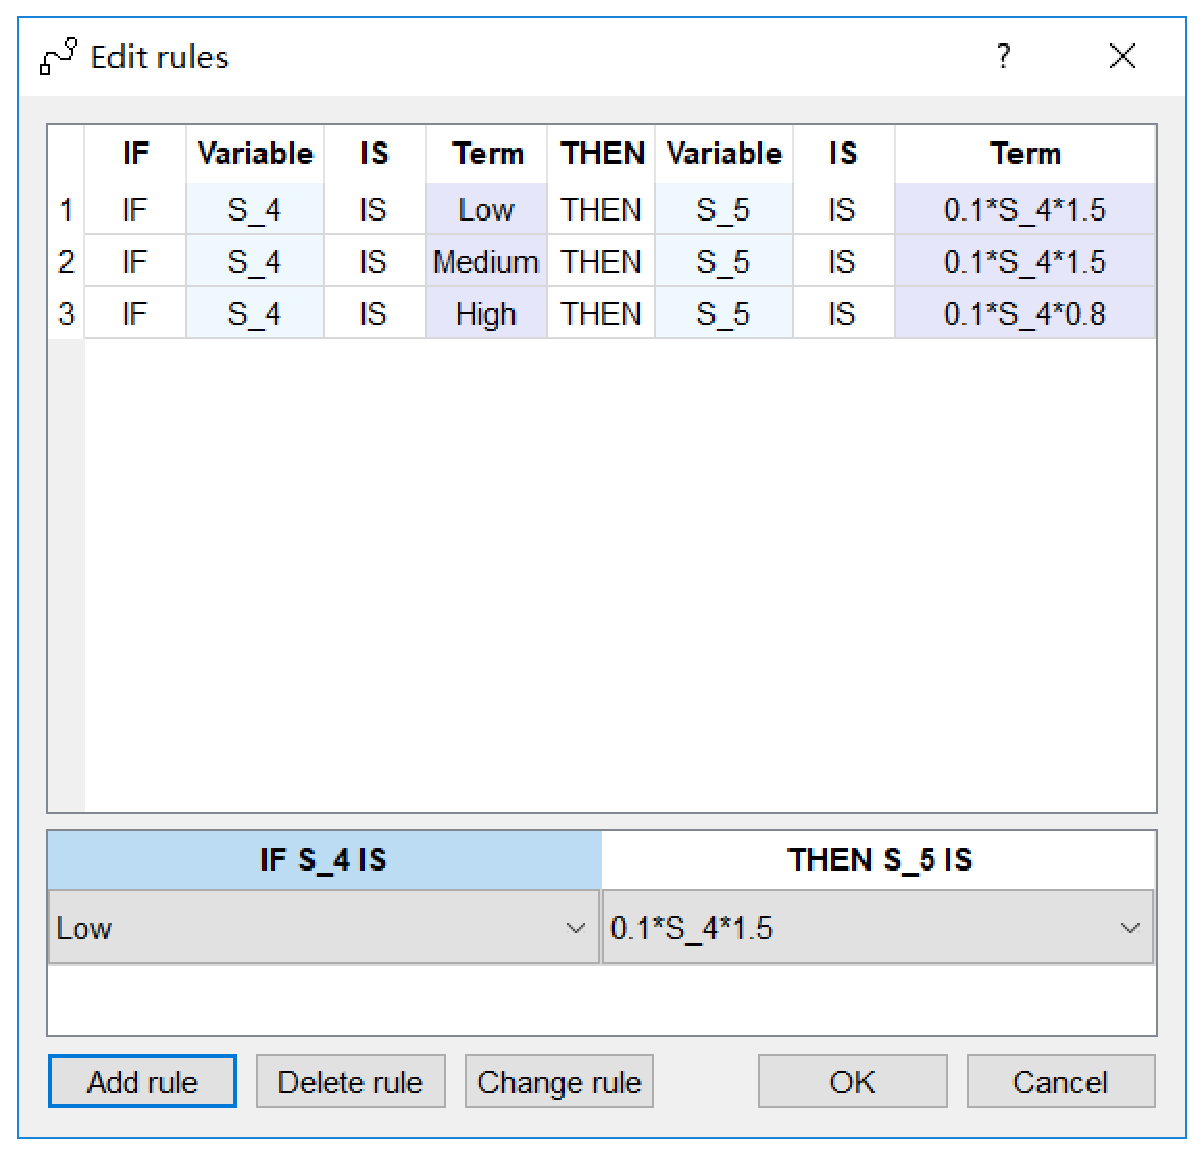
\includegraphics[width=\columnwidth]{fig35}
		\caption{Rules of the 1D Diffusion Reaction model using the T-S setting.}
		\label{fig:Rules of 1D Diffusion Reaction using T-S.}
	\end{center}
\end{figure}

\begin{figure}[!hbt]
	\begin{center}
		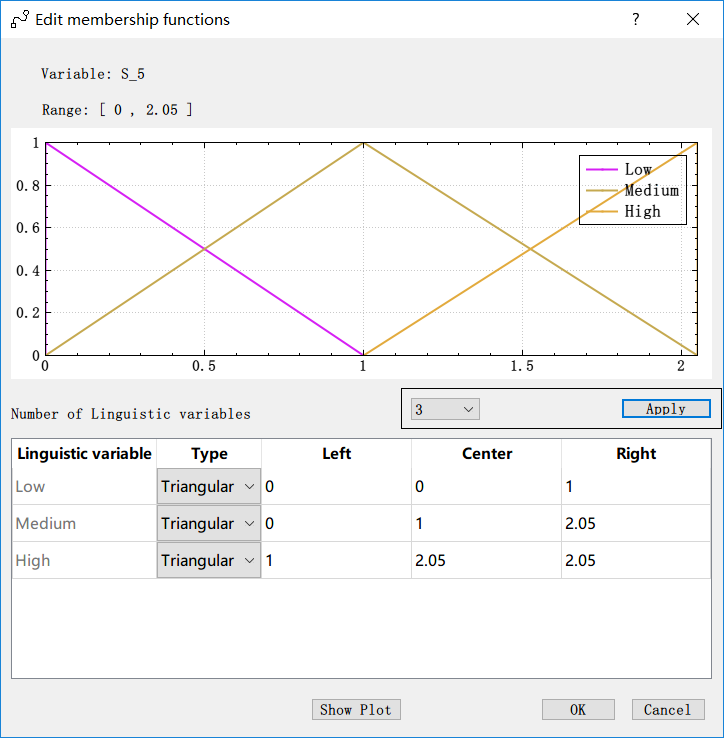
\includegraphics[width=0.45\columnwidth]{fig36}
		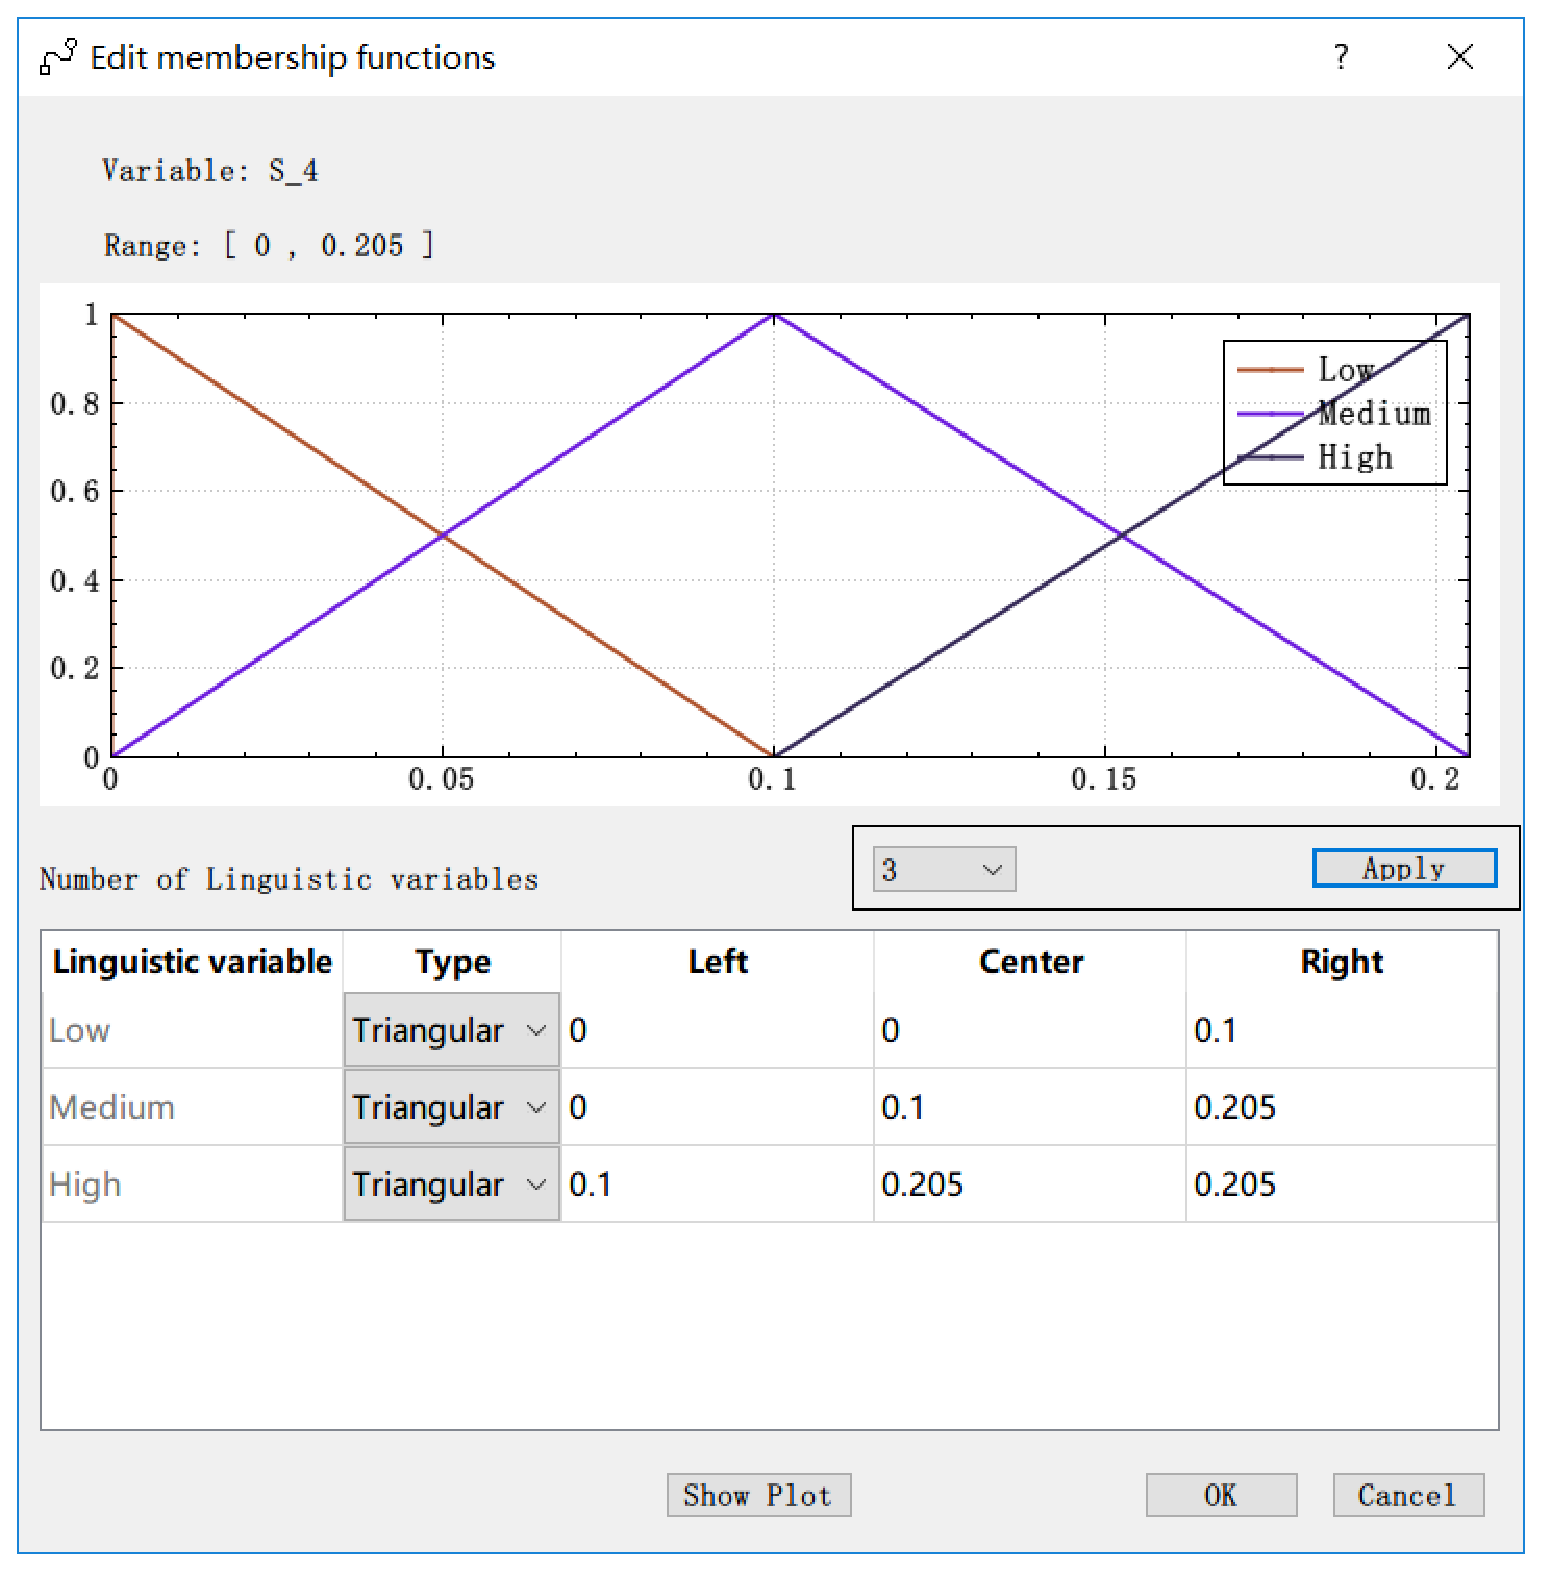
\includegraphics[width=0.45\columnwidth]{fig37}
		\caption{Membership functions of the 1D Diffusion Reaction model using the hybrid FIS setting (Mamdani).}
		\label{fig:Membership functions of 1D Diffusion Reaction using hybrid FIS (Mamdani).}
	\end{center}
\end{figure}

\begin{figure}[!hbt]
	\begin{center}
		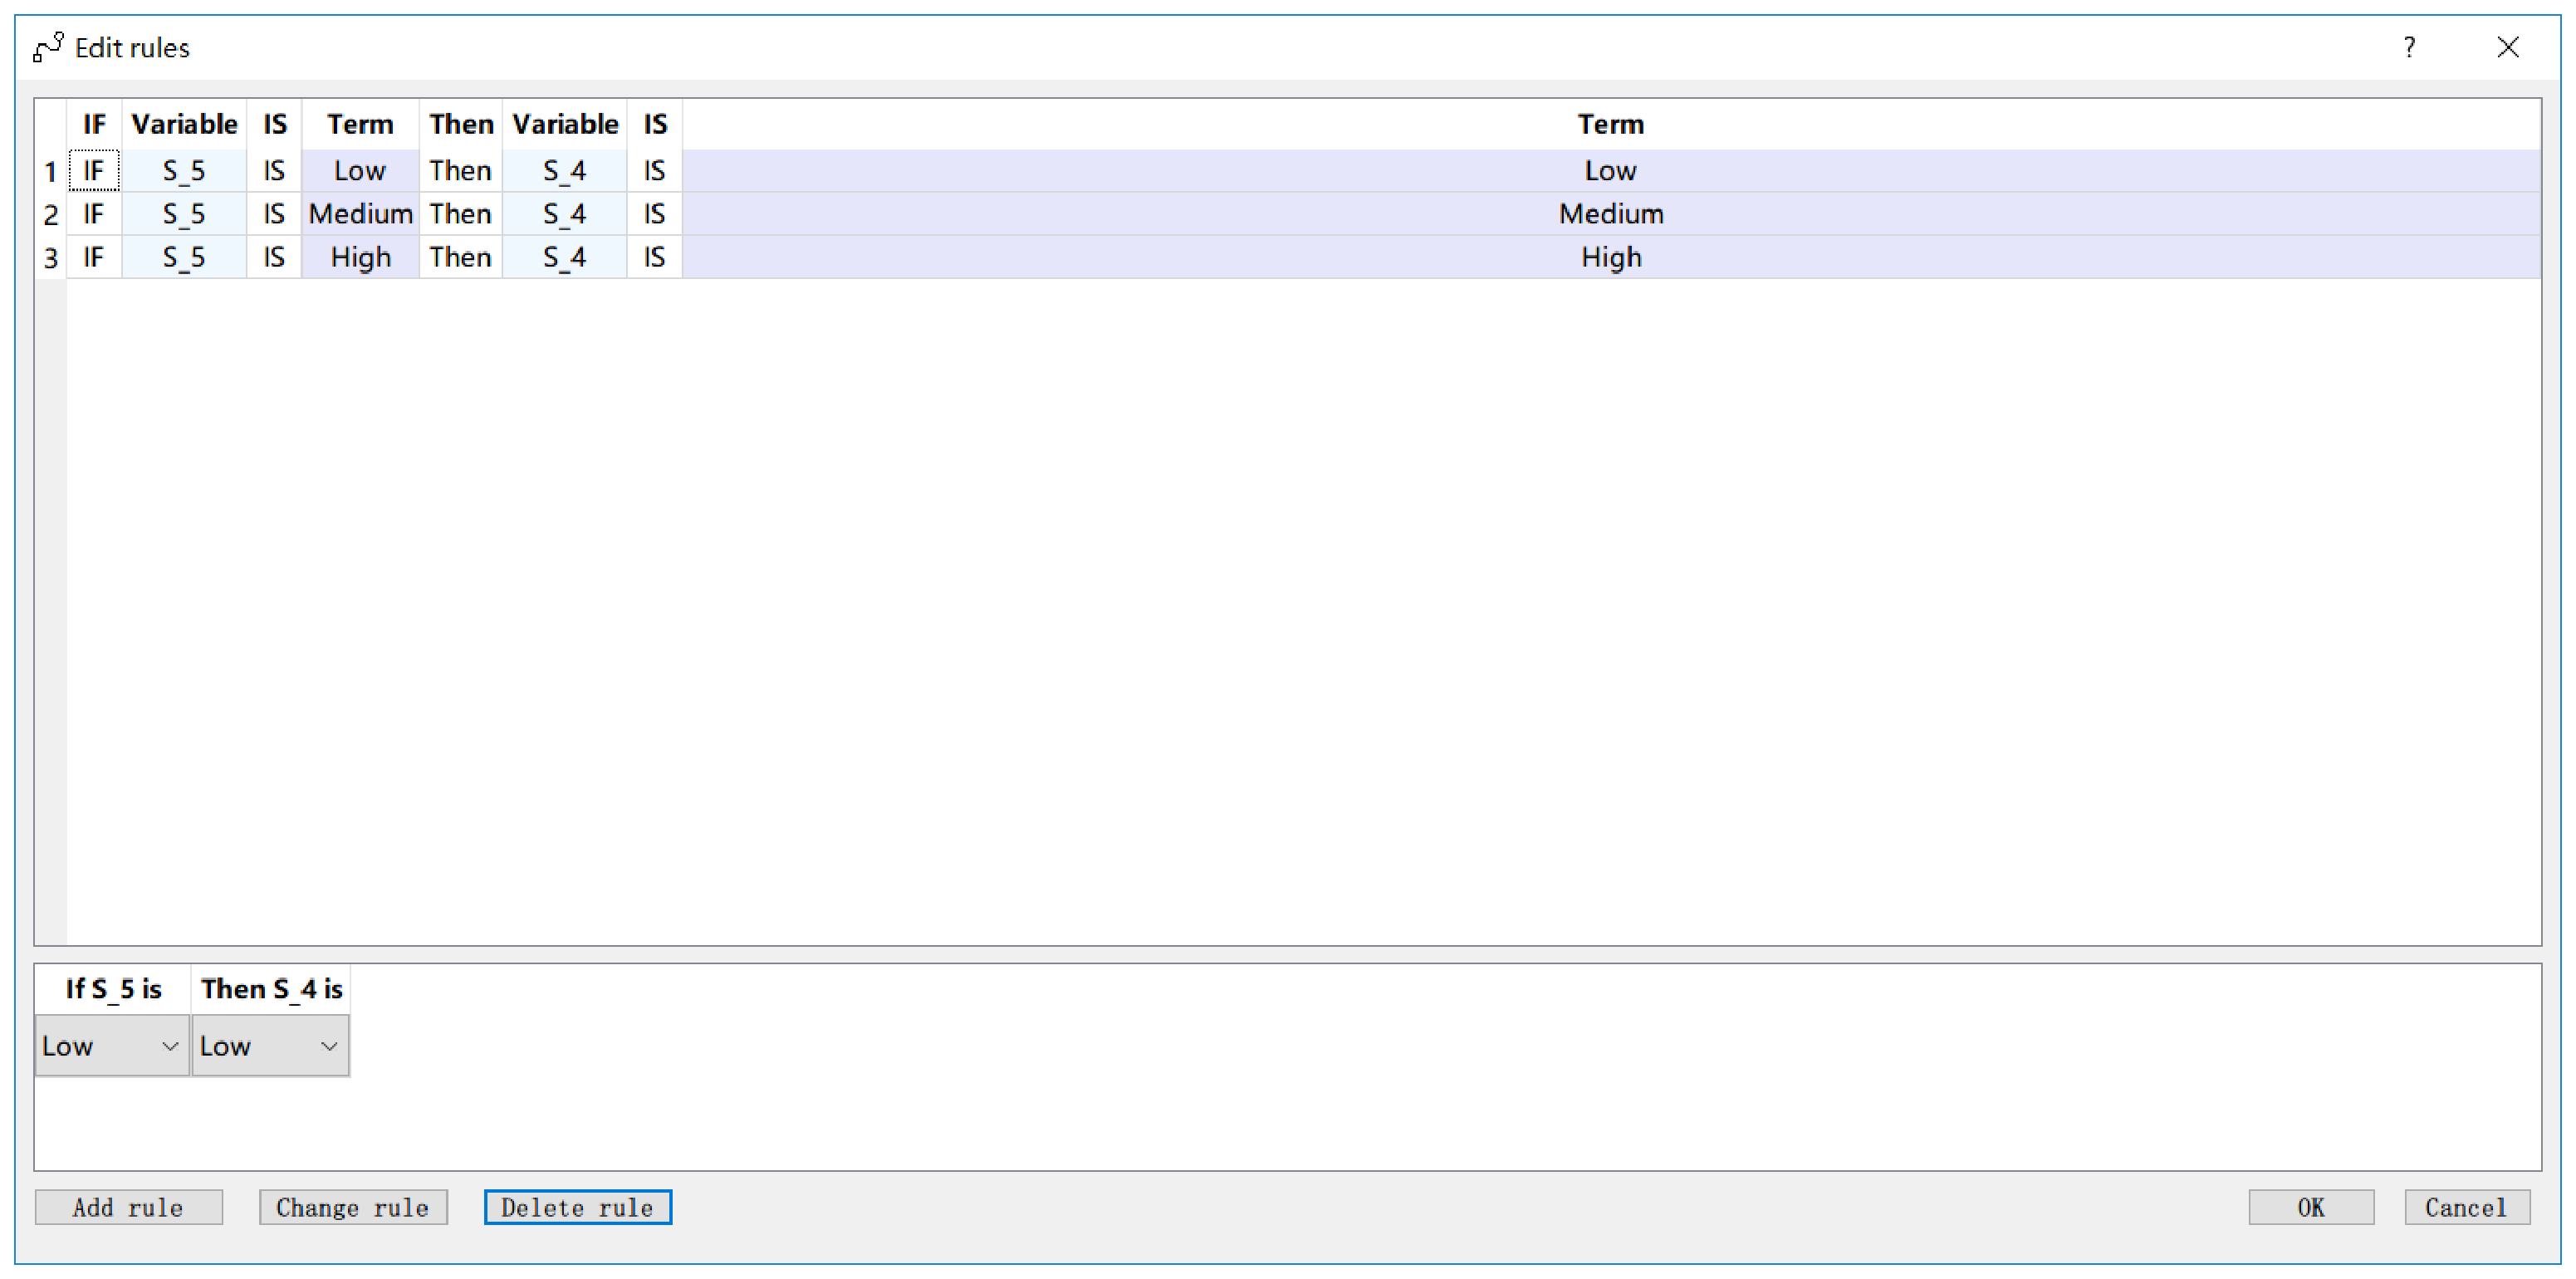
\includegraphics[width=\columnwidth]{fig38}
		\caption{Rules of the 1D Diffusion Reaction model using the hybrid FIS setting (Mamdani).}
		\label{fig:Rules of 1D Diffusion Reaction using hybrid FIS (Mamdani).}
	\end{center}
\end{figure}

\begin{figure}[!hbt]
	\begin{center}
		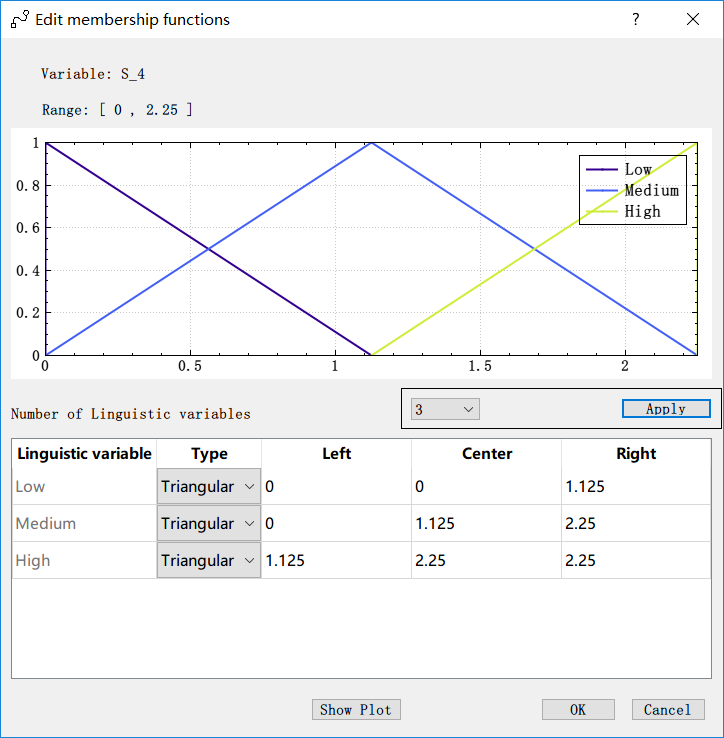
\includegraphics[width=0.9\columnwidth]{fig39}
		\caption{Membership functions of the 1D Diffusion Reaction model using the hybrid FIS setting (T-S).}
		\label{fig:Membership functions of 1D Diffusion Reaction using hybrid FIS (T-S).}
	\end{center}
\end{figure}

\begin{figure}[!hbt]
	\begin{center}
		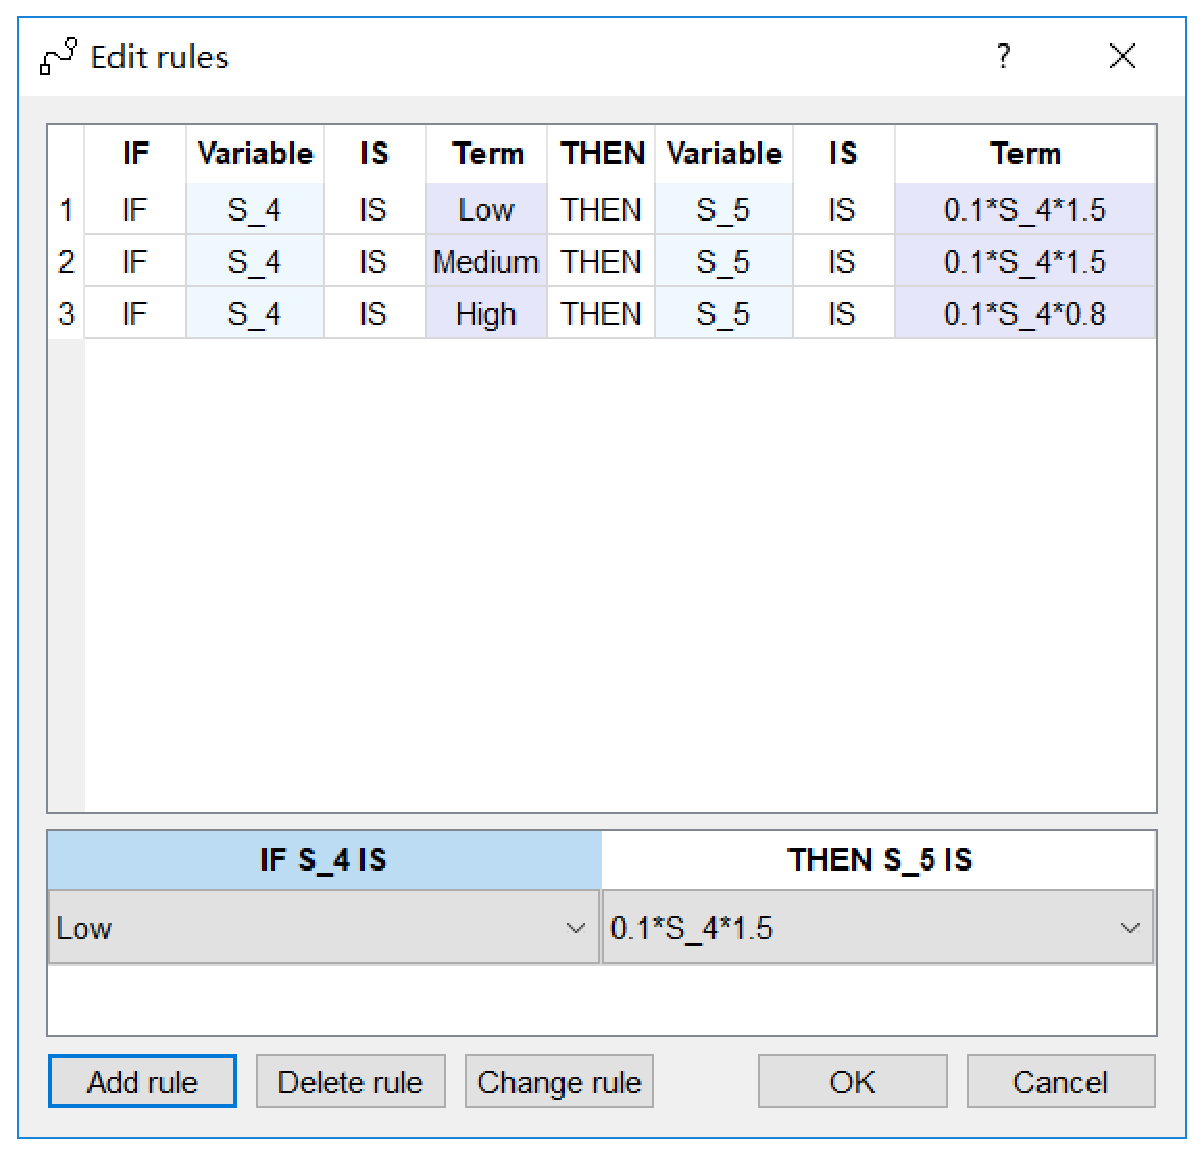
\includegraphics[width=\columnwidth]{fig40}
		\caption{Rules of the 1D Diffusion Reaction model using the hybrid FIS setting (T-S).}
		\label{fig:Rules of 1D Diffusion Reaction using hybrid FIS (T-S).}
	\end{center}
\end{figure}



\clearpage
\subsubsection{Simulation result}
In this example, we give the results of the four modes: no FIS (only ODEs), Mamdani, T-S, and hybrid FIS. The result of only ODEs is shown in Figure \ref{fig:Simulation result of 1D diffusion reaction using only ODEs.}.

When using the Mamdani setting, we choose to assign an FIS to the arc from t\_5\_4 to S\_4. The result is shown in Figure \ref{fig:Simulation result of 1D diffusion reaction using Mamdani.}.

When using T-S, we choose to assign an FIS to the arc the arc from t\_4\_5 to S\_5. The result is shown in Figure \ref{fig:Simulation result of 1D diffusion reaction using T-S.}.

When using hybrid FIS, we choose to assign an mamdani FIS to the arc from t\_5\_4 to S\_4 and to assign a T-S FIS to the arc from t\_4\_5 to S\_5. 
The result is shown in Figure \ref{fig:Simulation result of 1D diffusion reaction using hybrid FIS.}.

In the mode of only ODEs, the values of all variables eventually reach 2 while in the other three modes, the final values of the variables are not 2, but are very close to 2. And the trends of all four curves are consistent.

\begin{figure}[!hbt]
	\begin{center}
		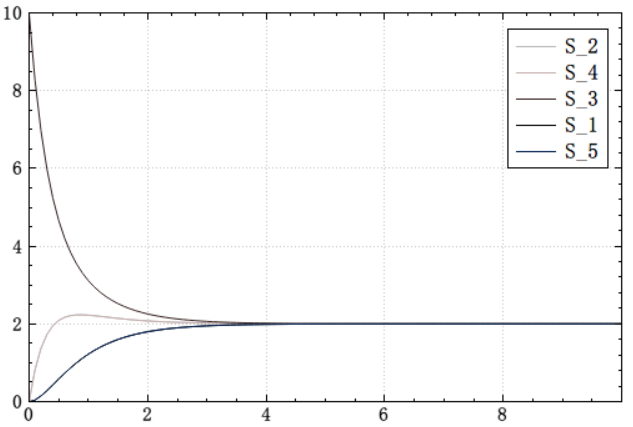
\includegraphics[width=\columnwidth]{fig21}
		\caption{Simulation result of 1D diffusion reaction using only ODEs.}
		\label{fig:Simulation result of 1D diffusion reaction using only ODEs.}
	\end{center}
\end{figure}

\begin{figure}[!hbt]
	\begin{center}
		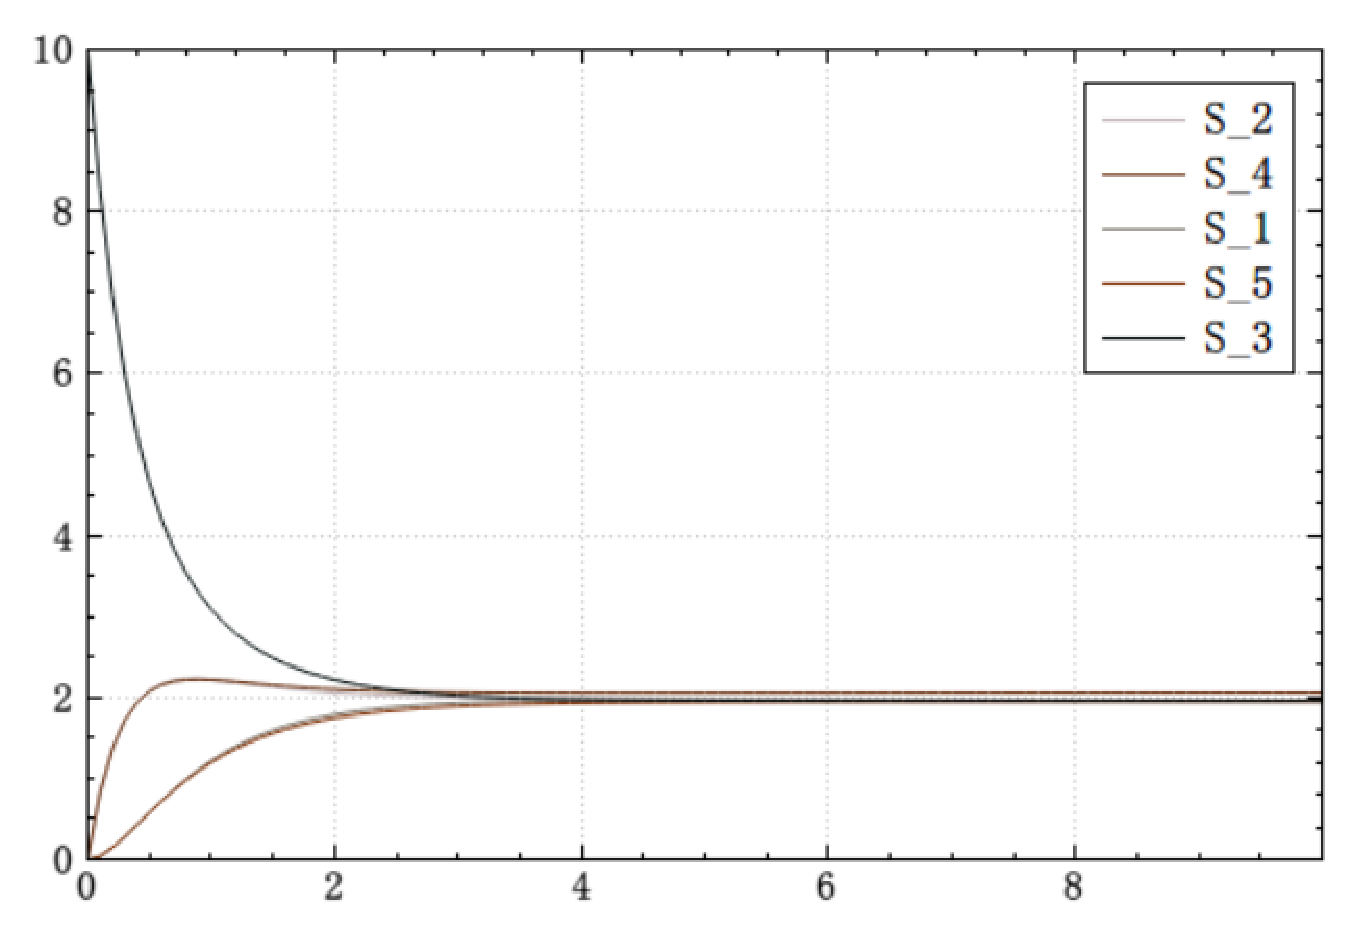
\includegraphics[width=\columnwidth]{fig22}
		\caption{Simulation result of 1D diffusion reaction using Mamdani.}
		\label{fig:Simulation result of 1D diffusion reaction using Mamdani.}
	\end{center}
\end{figure}

\begin{figure}[!hbt]
	\begin{center}
		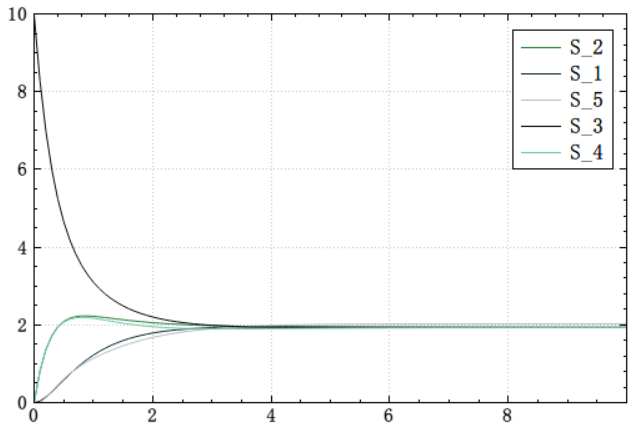
\includegraphics[width=\columnwidth]{fig23}
		\caption{Simulation result of 1D diffusion reaction using T-S.}
		\label{fig:Simulation result of 1D diffusion reaction using T-S.}
	\end{center}
\end{figure}

\begin{figure}[!hbt]
	\begin{center}
		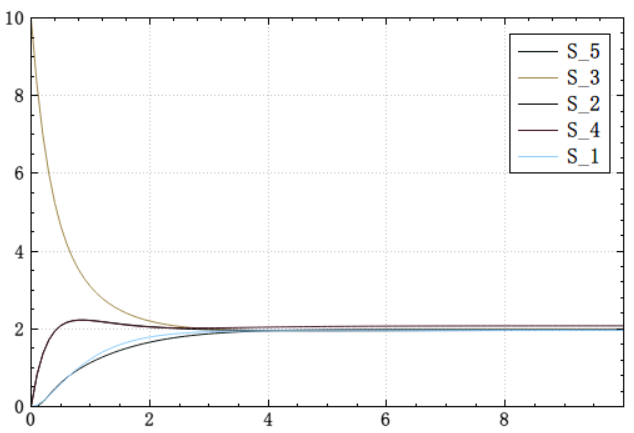
\includegraphics[width=\columnwidth]{fig24}
		\caption{Simulation result of 1D diffusion reaction using hybrid FIS.}
		\label{fig:Simulation result of 1D diffusion reaction using hybrid FIS.}
	\end{center}
\end{figure}



\clearpage
\subsection{Enzymatic reaction}

\subsubsection{Introduction}
The second example is enzymatic reaction \cite{BHM11}. Enzymes are macromolecular biological catalysts, which can accelerate chemical reactions. The molecules upon which enzymes may act are called substrates and the enzyme converts the substrates into different molecules, known as products. Almost all metabolic processes in a cell need enzyme catalysis in order to occur at rates fast enough to sustain life. Metabolic pathways depend upon enzymes to catalyze individual steps. 

\subsubsection{Model}
The model is shown in Figure \ref{fig:The model of enzyme}.

\begin{figure}[!hbt]
	\begin{center}
		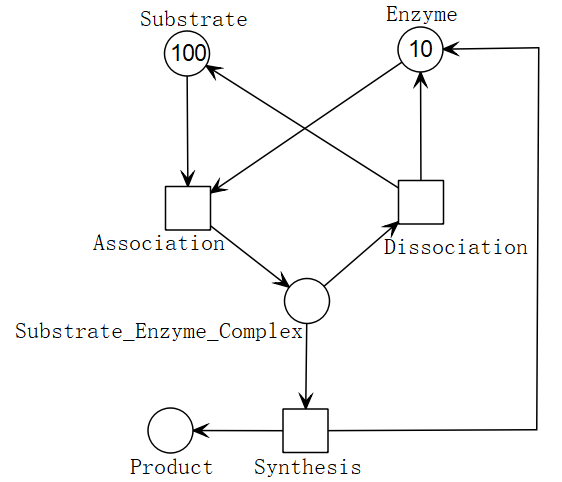
\includegraphics[width=0.8\columnwidth]{fig25}
		\caption{The model of enzymatic reaction.}
		\label{fig:The model of enzyme}
	\end{center}
\end{figure}

\begin{table}[!hbt]
	\begin{center}
		\caption{Transition functions of the enzymatic reaction model.}
		\label{Transition functions of enzyme}
		\begin{tabular}{|c|c|}
			\hline
			Transition&Function\\
			\hline
			Assoication&MassAction(0.1)\\
			\hline
			Dissociation&MassAction(0.1)\\
			\hline
			Synthesis&MassAction(0.1)\\
			\hline
		\end{tabular}
	\end{center}
\end{table}

\begin{figure}[!hbt]
	\begin{center}
		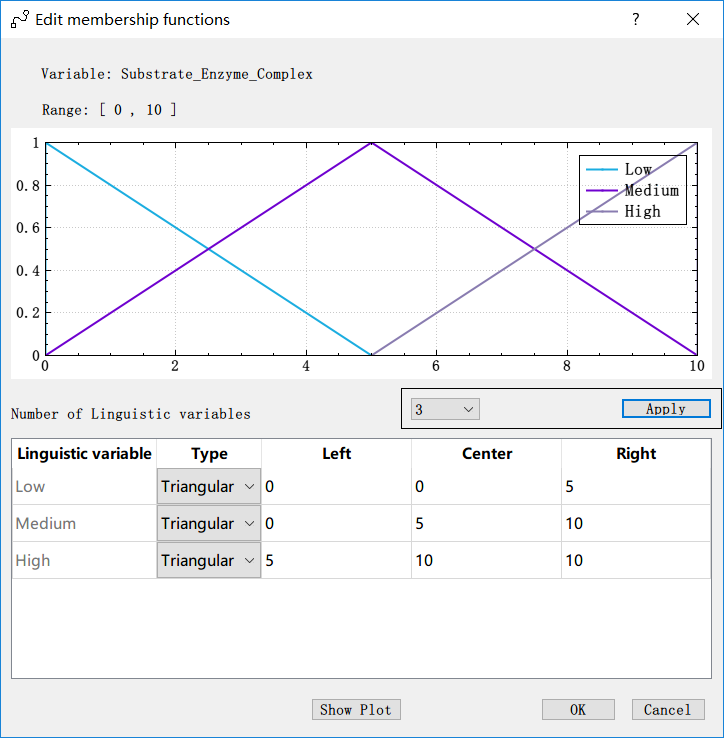
\includegraphics[width=0.45\columnwidth]{fig41}
		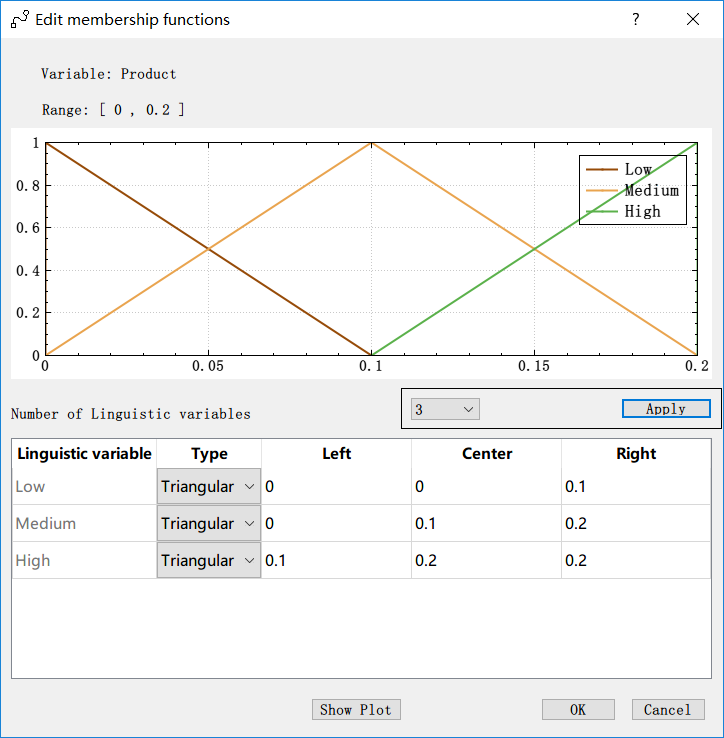
\includegraphics[width=0.45\columnwidth]{fig42}
		\caption{Membership functions of the enzymatic reaction model using the Mamdani setting.}
		\label{fig:Membership functions of enzyme using Mamdani.}
	\end{center}
\end{figure}

\begin{figure}[!hbt]
	\begin{center}
		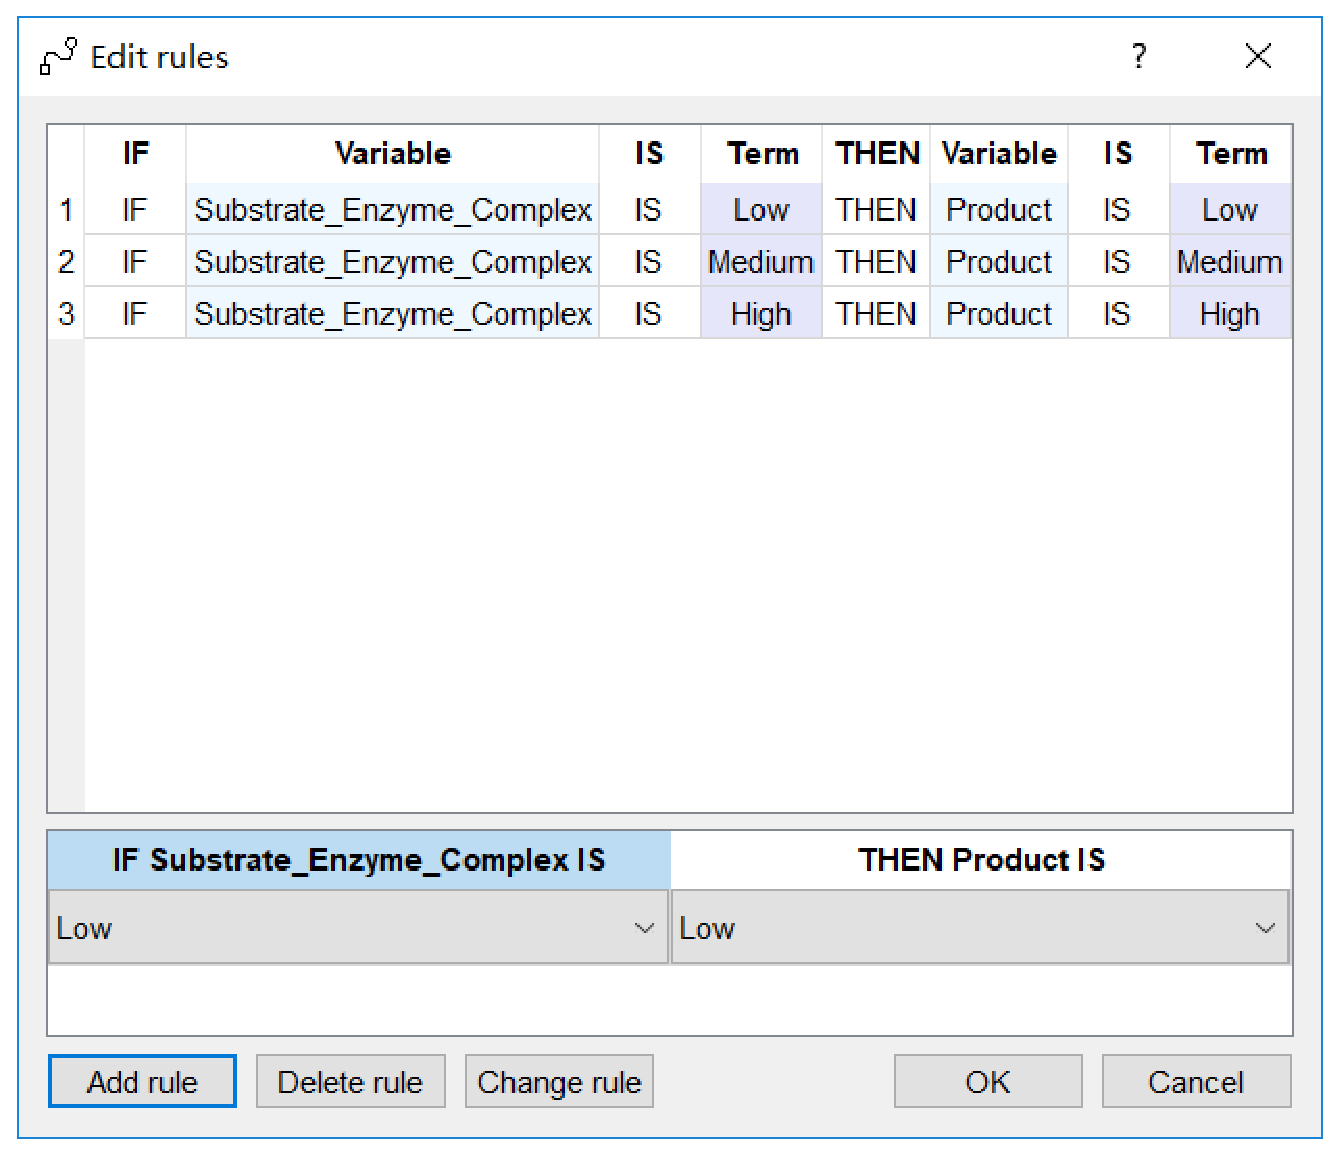
\includegraphics[width=\columnwidth]{fig43}
		\caption{Rules of the enzymatic reaction model using the Mamdani setting.}
		\label{fig:Rules of enzyme using Mamdani.}
	\end{center}
\end{figure}

\subsubsection{Simulation result}
In this example, we give the result of two modes: only ODEs and Mamdani. The result of only ODEs is shown in Figure \ref{fig:Simulation result of enzyme using only ODEs.}.

When using the Mamdani setting, we choose to assign an FIS to the arc from Synthesis to Product. The result is shown in Figure \ref{fig:Simulation result of enzyme using Mamdani.}.

As we can see, the results are almost the same.

\begin{figure}[!hbt]
	\begin{center}
		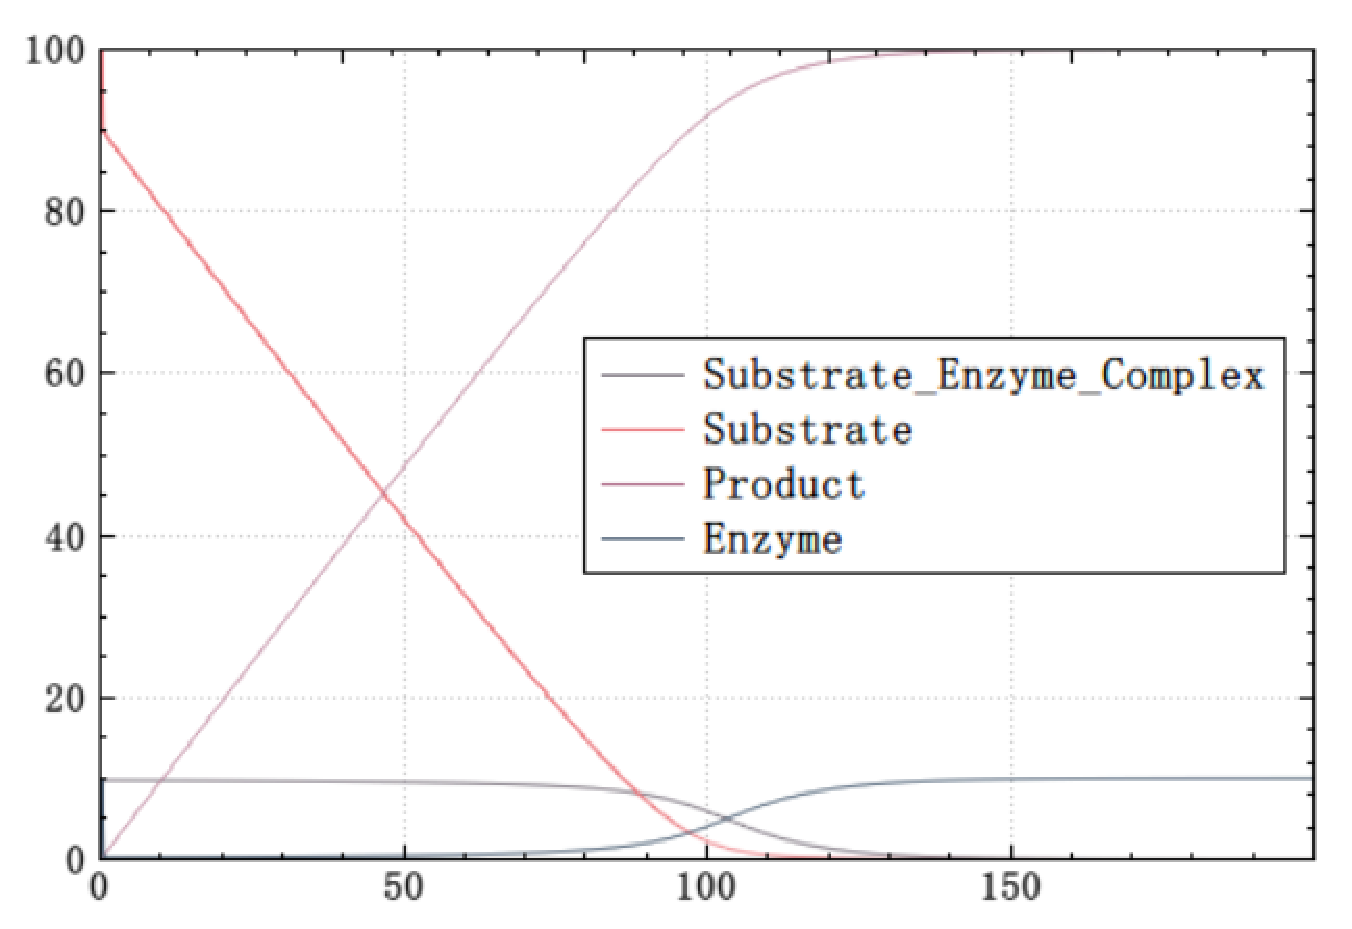
\includegraphics[width=\columnwidth]{fig26}
		\caption{Simulation result of the enzymatic reaction model using only ODEs.}
		\label{fig:Simulation result of enzyme using only ODEs.}
	\end{center}
\end{figure}

\begin{figure}[!hbt]
	\begin{center}
		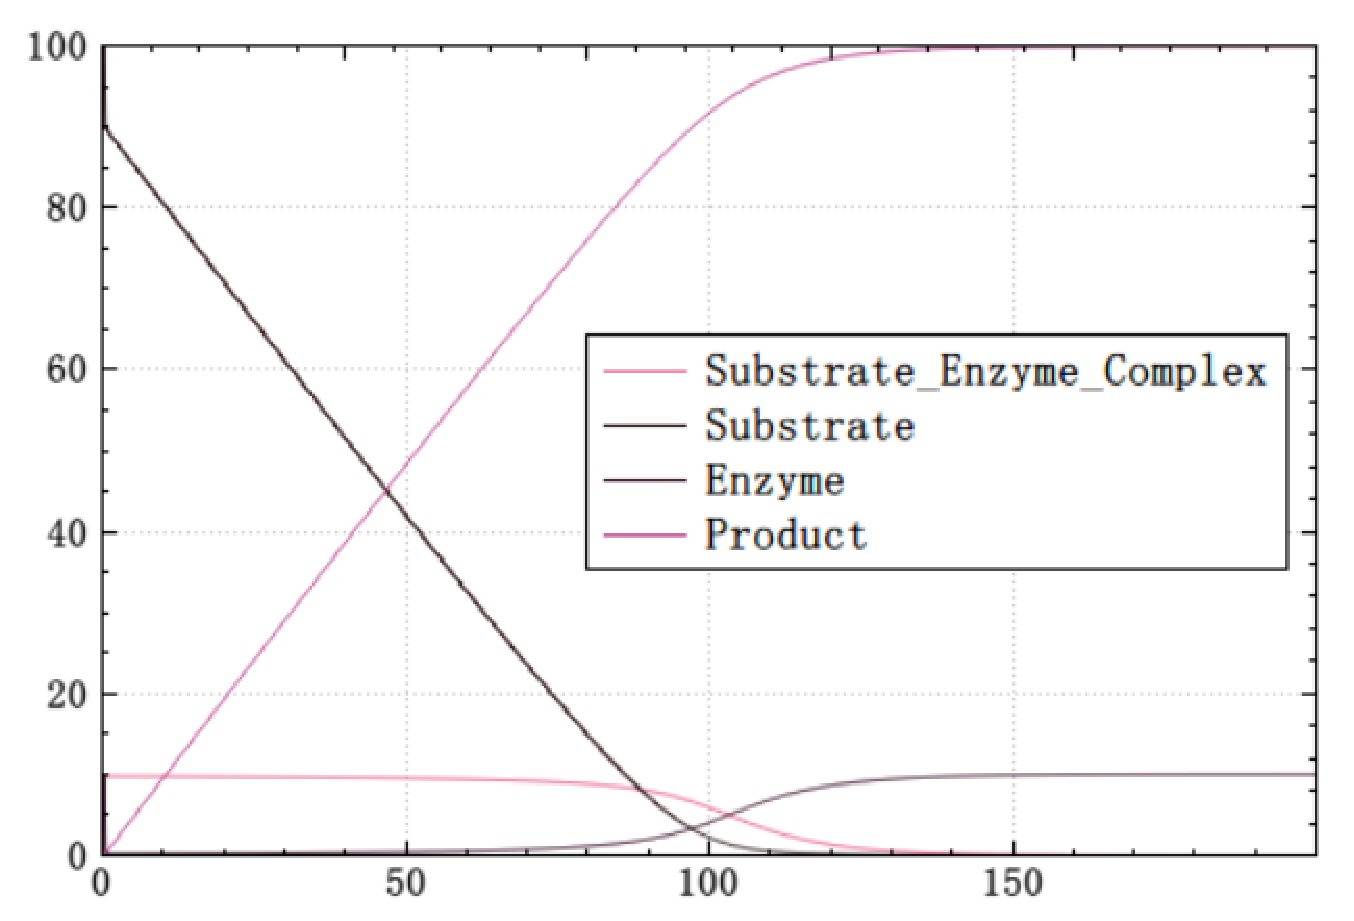
\includegraphics[width=\columnwidth]{fig27}
		\caption{Simulation result of the enzymatic reaction model using the Mamdani setting.}
		\label{fig:Simulation result of enzyme using Mamdani.}
	\end{center}
\end{figure}





\clearpage
\subsection{RKIP pathway}

\subsubsection{Introduction}

The Raf kinase inhibitor protein (RKIP) \cite{CSK+03} is a kinase inhibitor protein that regulates many signaling pathways within the cell. RKIP is a member of the phosphatidylethanolamine-binding protein family and has displayed disruptive regulation on the Raf-1-MEK1/2, ERK1/2 and NF-kappaB signalling pathways, by interaction with the Raf-1 kinase. 

\subsubsection{Model}
The model is shown in Figure \ref{fig:The model of RKIP}, based on the CPN model given in \cite{GH06}.

\begin{figure}[!hbt]
	\begin{center}
		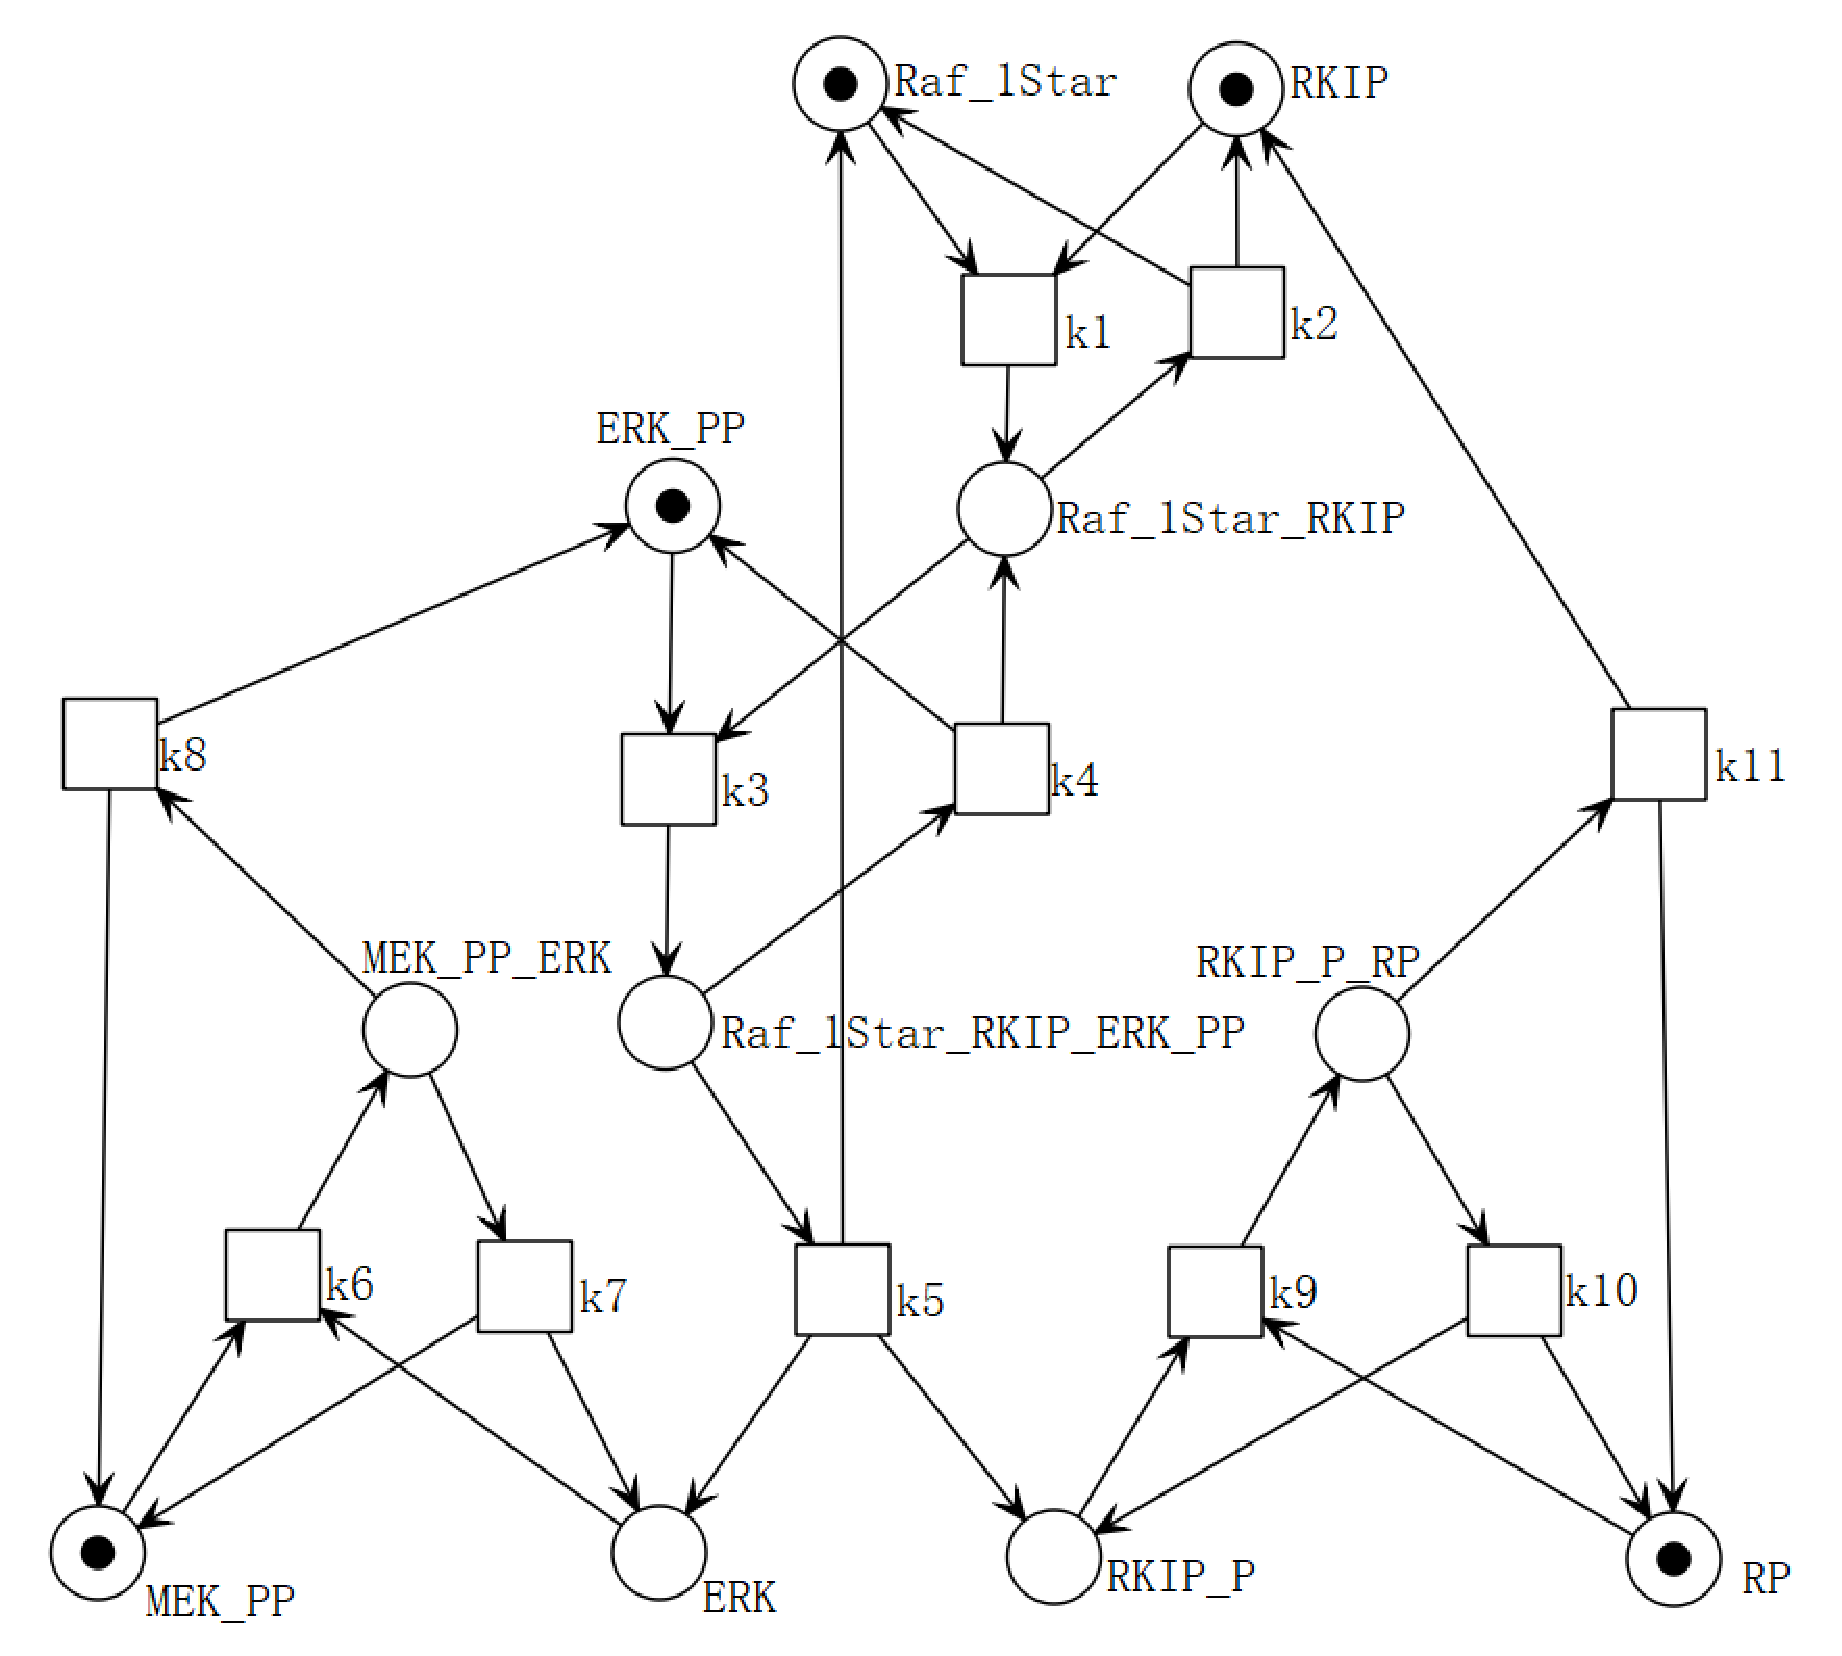
\includegraphics[width=\columnwidth]{fig28}
		\caption{The model of the RKIP pathway.}
		\label{fig:The model of RKIP}
	\end{center}
\end{figure}

\begin{table}[!hbt]
	\begin{center}
		\caption{Transition functions of the RKIP pathway model.}
		\label{Transition functions of RKIP}
		\begin{tabular}{|c|c|}
			\hline
			Transition&Function\\
			\hline
			k1&MassAction(0.53)\\
			\hline
						k2&MassAction(0.0072)\\
			\hline
						k3&MassAction(0.625)\\
			\hline
						k4&MassAction(0.00245)\\
			\hline
						k5&MassAction(0.0315)\\
			\hline
						k6&MassAction(0.6)\\
			\hline
						k7&MassAction(0.0075)\\
			\hline
						k8&MassAction(0.071)\\
			\hline
						k9&MassAction(0.92)\\
			\hline
						k10&MassAction(0.00122)\\
			\hline
						k11&MassAction(0.87)\\
			\hline
		\end{tabular}
	\end{center}
\end{table}

\begin{figure}[!hbt]
	\begin{center}
		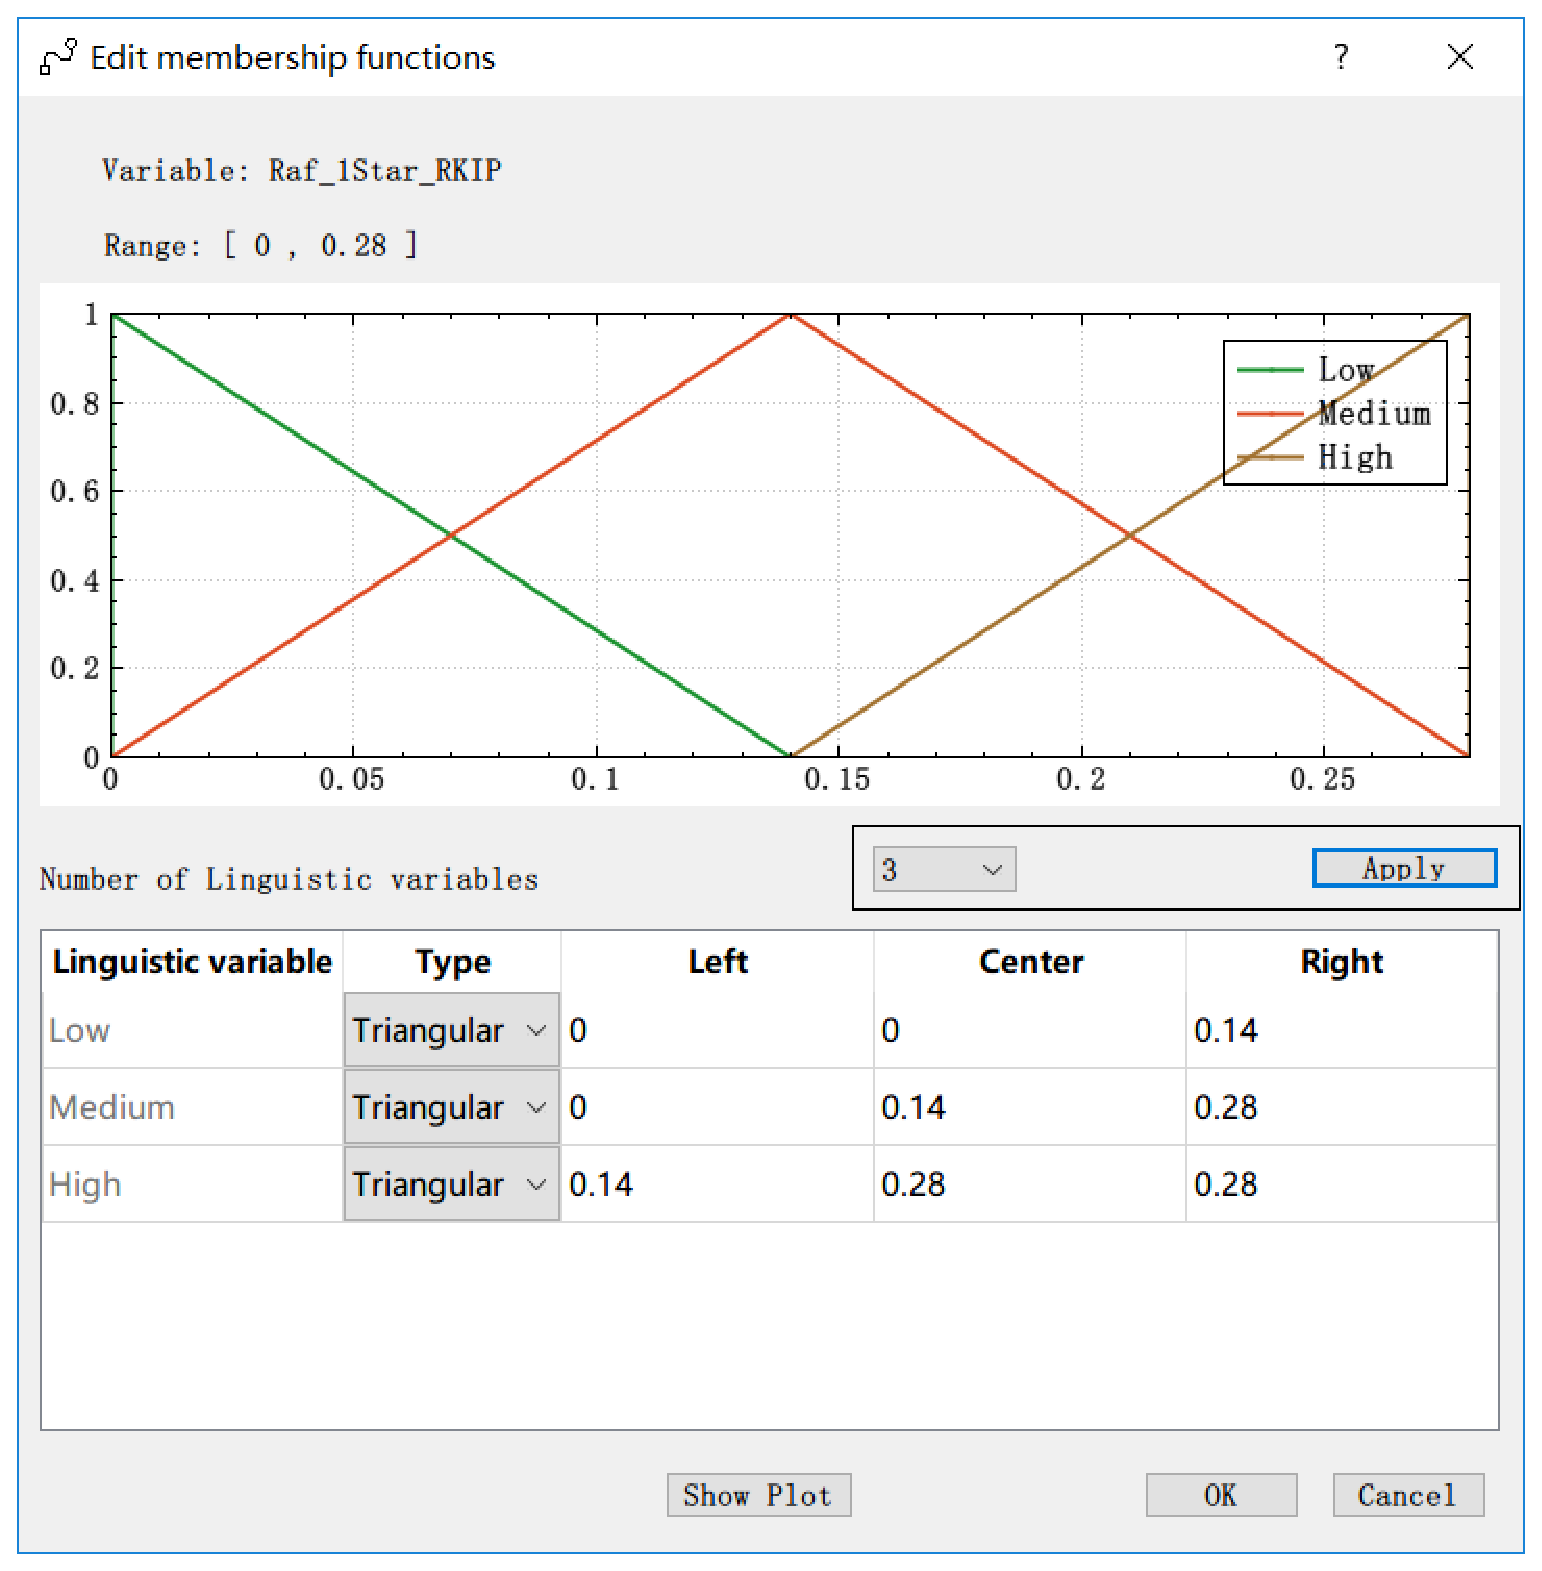
\includegraphics[width=0.45\columnwidth]{fig44}
		\includegraphics[width=0.45\columnwidth]{fig45}
		\caption{Membership functions of the RKIP pathway model using the T-S setting.}
		\label{fig:Membership functions of RKIP using T-S.}
	\end{center}
\end{figure}

\begin{figure}[!hbt]
	\begin{center}
		\includegraphics[width=\columnwidth]{fig46}
		\caption{Rules of the RKIP pathway model using the T-S setting.}
		\label{fig:Rules of RKIP using T-S.}
	\end{center}
\end{figure}


\subsubsection{Simulation result}
In this example, we give the results of the modes: only ODEs and T-S. The result of only ODEs is shown in Figure \ref{fig:Simulation result of RKIP using only ODEs.}.

When using T-S, we choose to assign an FIS to the arc from k3 to Raf\_1Star\_RKIP\_ERK\_PP. The result is shown in Figure \ref{fig:Simulation result of RKIP using T-S.}.

As we can see, the results are almost consistent. Pay attention to the bold blue curves of Figure \ref{fig:Simulation result of RKIP using only ODEs.} and Figure \ref{fig:Simulation result of RKIP using T-S.}. The final result is a little different. But we can adjust the rules to get a better result.

\begin{figure}[!hbt]
	\begin{center}
		\includegraphics[width=\columnwidth]{fig29}
		\caption{Simulation result of the RKIP pathway model using only ODEs.}
		\label{fig:Simulation result of RKIP using only ODEs.}
	\end{center}
\end{figure}

\begin{figure}[!hbt]
	\begin{center}
		\includegraphics[width=\columnwidth]{fig30}
		\caption{Simulation result of the RKIP pathway model using the T-S setting.}
		\label{fig:Simulation result of RKIP using T-S.}
	\end{center}
\end{figure}





\clearpage
\subsection{6-mercaptopurine metabolism}
\subsubsection{Introduction}
6-Mercaptopurine (6-MP) is one of the important chemotherapy drugs used for treating acute lymphocytic leukaemia (ALL). According to the model given in \cite{lavrova2017ordinary,lavrova2016ode}, we build the FCPN model of the 6-mercaptopurine metabolism.

\subsubsection{Model}
The model is shown in Figure \ref{fig:The model of 6-MP metabolism}.

\begin{figure}[!hbt]
	\begin{center}
		\includegraphics[width=\columnwidth]{fig53}
		\caption{The model of 6-MP metabolism.}
		\label{fig:The model of 6-MP metabolism}
	\end{center}
\end{figure}

\begin{table}[!hbt]
	\begin{center}
		\caption{Transition functions of the 6-MP metabolism model.}
		\label{Transition functions of 6-MP metabolism}
		\begin{tabular}{|c|c|}
			\hline
			Transition&Function\\
			\hline
			k0&MassAction(5)\\
			\hline
			k1&MassAction(10)\\
			\hline
			k\_1&MassAction(0.01)\\
			\hline
			k2&MassAction(10)\\
			\hline
			k\_2&MassAction(4)\\
			\hline
			k3&MassAction(5)\\
			\hline
			k\_3&MassAction(0.01)\\
			\hline
			k4&MassAction(0.00001)\\
			\hline
			k\_4&MassAction(0.1)\\
			\hline
			k7&MassAction(0.01)\\
			\hline
			k\_7&MassAction(1)\\
			\hline
			k8&MassAction(0.5)\\
			\hline
			k\_8&MassAction(0.01)\\
			\hline
			VPUR&MassAction(0.01)\\
			\hline
			VD&MassAction(0.9)\\
			\hline
			VOUT&MassAction(0.0001)\\
			\hline
		\end{tabular}
	\end{center}
\end{table}


\begin{figure}[!hbt]
	\begin{center}
		\includegraphics[width=0.45\columnwidth]{fig57}
		\includegraphics[width=0.45\columnwidth]{fig58}
		\caption{Membership functions of the 6-MP metabolism model using the Mamdani setting.}
		\label{fig:Membership functions of 6-MP metabolism using Mamdani.}
	\end{center}
\end{figure}

\begin{figure}[!hbt]
	\begin{center}
		\includegraphics[width=\columnwidth]{fig59}
		\caption{Rules of the 6-MP metabolism model using the Mamdani setting.}
		\label{fig:Rules of 6-MP metabolism using Mamdani.}
	\end{center}
\end{figure}
\begin{figure}[!hbt]
	\begin{center}
		\includegraphics[width=\columnwidth]{fig57}
		\caption{Membership functions of the 6-MP metabolism model using the T-S setting.}
		\label{fig:Membership functions of 6-MP metabolism using T-S.}
	\end{center}
\end{figure}

\begin{figure}[!hbt]
	\begin{center}
		\includegraphics[width=\columnwidth]{fig60}
		\caption{Rules of the 6-MP metabolism model using the T-S setting.}
		\label{fig:Rules of 6-MP metabolism using T-S.}
	\end{center}
\end{figure}


\subsubsection{Simulation result}
In this example, we give the results of three modes: only ODEs, Mamdani, and T-S. The result of only ODEs is shown in Figure \ref{fig:Simulation result of 6-MP metabolism using only ODEs.}.

When using Mamdani, we choose to assign an FIS to the arc from k0 to MPin. The result is shown in Figure \ref{fig:Simulation result of 6-MP metabolism using Mamdani.}.

When using T-S, we choose to assign an FIS to the arc from k0 to MPin. The result is shown in Figure \ref{fig:Simulation result of 6-MP metabolism using T-S.}.

As we can see, the results are almost the same.

\begin{figure}[!hbt]
	\begin{center}
		\includegraphics[width=\columnwidth]{fig54}
		\caption{Simulation result of the 6-MP metabolism model using only ODEs.}
		\label{fig:Simulation result of 6-MP metabolism using only ODEs.}
	\end{center}
\end{figure}

\begin{figure}[!hbt]
	\begin{center}
		\includegraphics[width=\columnwidth]{fig55}
		\caption{Simulation result of the 6-MP metabolism model using the Mamdani setting.}
		\label{fig:Simulation result of 6-MP metabolism using Mamdani.}
	\end{center}
\end{figure}

\begin{figure}[!hbt]
	\begin{center}
		\includegraphics[width=\columnwidth]{fig56}
		\caption{Simulation result of the 6-MP metabolism model using the T-S setting.}
		\label{fig:Simulation result of 6-MP metabolism using T-S.}
	\end{center}
\end{figure}


\clearpage


\section{Combine FCPN with neuro-fuzzy system}
\subsection{Introduction}
Since some parameters of fuzzy sets of Mamdani and T-S are not easy to determine, some experts have proposed a method of using neural networks to train datas to obtain fuzzy set parameters and rules \cite{jang1993anfis}\cite{Xiao2015Research}.

In order to make it easier for users to train and get relevant parameters, we have added the function of automatically exporting .m files in the software. Users only need to open the file with MATLAB, fill in the relevant data, and run it to get the result.
\subsection{Instruction}
\subsubsection{Output the file}
If you want to output the .m file, you should follow the instruction in section 2.2. It does not matter if you are not sure about the correct parameters. However, make sure to fill in the appropriate rules which will be used in MATLAB. Of course, you can edit the rules in MATLAB as well. After that, you will get a result like Figure \ref{fig:Output the file.}.

Left click the ``Output to .m file'' button to output the file.
\begin{figure}[!hbt]
	\begin{center}
		\includegraphics[width=\columnwidth]{fig61}
		\caption{Output the file.}
		\label{fig:Output the file.}
	\end{center}
\end{figure}
\subsubsection{Train datas in MATLAB}
\begin{itemize}
	\item \textbf{Mamdani}
	
	If the type of FIS is Mamdani, you will get two files. The comment content describes the variables to help you understand the code better.
	
	Part of the code in the file is similar to Figure \ref{fig:Part of the code in Mamdani type file.}.
	\begin{figure}[!hbt]
		\begin{center}
			\includegraphics[width=\columnwidth]{fig62}
			\caption{Part of the code in Mamdani type file.}
			\label{fig:Part of the code in Mamdani type file.}
		\end{center}
	\end{figure}
	You should import the training datas to \textbf{input\_train} and \textbf{out\_train} using \textbf{csvread('data.csv')} or something like this. The \textbf{train\_m} and \textbf{train\_sigma} should also be editted by yourself. Make sure the orders of input datas should be consistent with \textbf{input\_train}, \textbf{train\_m}, \textbf{train\_sigma}, and \textbf{rules}.
	
	\textbf{rate, epoch($\eta$), a, b, kk} can also be editted to achieve better result. The following equation illustrates the role of a, b, and kk.
	
	\begin{equation}    
	\eta =
	\begin{cases}
	a*\eta   &  \text{E(t+1)/E(t) < 1} \\
	b*\eta	 &  \text{E(t+1)/E(t) $\ge$ kk}\\
	\eta     &  \text{other}
	\end{cases}                
	\end{equation}
	where E(t+1) is the new error and E(t) is the old error.
	
	In the end, run the code to get the trained parameters and fill them in FCPN. Make sure the type of membership functions should be selected as \textbf{Gauss} and the AND Method should be consistent with the \textbf{andMethod} in MATLAB.

	\item \textbf{T-S}
	
	If the type of FIS is T-S, you will get one file. The comment content describes the variables to help you understand the code better.
	
	Part of the code in the file is similar to Figure \ref{fig:Part of the code in T-S type file.}.
	\begin{figure}[!hbt]
		\begin{center}
			\includegraphics[width=\columnwidth]{fig63}
			\caption{Part of the code in T-S type file.}
			\label{fig:Part of the code in T-S type file.}
		\end{center}
	\end{figure}

	You should import the training datas to \textbf{trnData} using \textbf{csvread('data.csv')} or something like this. Make sure the output data should be in the last column. 
	
	You can also adjust the \textbf{epoch}.
	
	In the end, run the code to get the trained parameters and fill them in FCPN. Make sure the type of membership functions should be selected as \textbf{Gauss} and the AND Method should be selected as \textbf{Product}.
	
\end{itemize}
\clearpage
%\section{References}
\bibliographystyle{unsrt}

\bibliography{ref} 
%\noindent
%[1] Petri net: \url{https://en.wikipedia.org/wiki/Petri_net}\newline
%[2] Fuzzy logic: \url{https://en.wikipedia.org/wiki/Fuzzy_logic}\newline
%[3] Fuzzy Inference Process: \url{https://www.mathworks.com/help/fuzzy/fuzzy-inference-process.html}\newline
%[4] Mamdani-Type Fuzzy Inference: \url{https://www.mathworks.com/help/fuzzy/what-is-mamdani-type-fuzzy-inference.html}\newline
%[5] Sugeno-Type Fuzzy Inference: \url{https://www.mathworks.com/help/fuzzy/what-is-sugeno-type-fuzzy-inference.html}\newline
%[6] Enzyme: \url{https://en.wikipedia.org/wiki/Enzyme}\newline
%[7] Raf kinase inhibitor protein: \url{https://en.wikipedia.org/wiki/Raf_kinase_inhibitor_protein}



\end{document}

